\chapter{Euklidiese meetkunde}
\setcounter{figure}{1}
\setcounter{subfigure}{1}
% \section{Meetkunde hersiening}
% \setcounter{figure}{1}
% \setcounter{subfigure}{1}

Meetkunde (Grieks: geo = aarde, metria = meet) het ontstaan as die veld van kennis van ruimtelike verbande.
Dit was een van die twee velde van pre-moderne wiskunde. Die ander veld was die studie van getalle. In
die moderne tyd het meetkundige begrippe baie kompleks en abstrak geraak en is dit skaars herkenbaar as ’n
uitvloeisel van vroëre meetkunde.\par 


\chapterstartvideo{VMchw}

% Die doel van hierdie hoofstuk is om van die meetkundige en trigonometriese konsepte, wat jy al in vroeëre grade
% teëgekom het, te hersien. Jy moet gemaklik wees met die werk wat behandel word in die hoofstuk voor jy die
% Graad 10 Meetkunde Hoofstuk\footnote{\raggedright{}"Geometry - Grade 10" <http://http://cnx.org/content/m32629/latest/>}, \footnote{\raggedright{}"Trigonometry - Grade 10" <http://http://cnx.org/content/m32620/latest/>} or the Grade 10 Analytical Geometry chapter\footnote{\raggedright{}"Analytical Geometry - Grade 10 [CAPS]" <http://http://cnx.org/content/m38370/latest/>}. Die hoofstuk hersien die
% volgende:\par 
% \begin{enumerate}[noitemsep, label=\textbf{\arabic*}. ] 
% \item Terminologie: vierhoeke, hoekpunte, sye, hoeke, parallele lyne, loodregte lyne, hoeklyne, halveerlyne en
% snylyne
% \item Eienskappe van driehoeke en vierhoeke
% \item Kongruensie
% \item Onderskeid tussen skerphoeke, regte hoeke, stomphoeke, reguitlyne en ’n volle omwenteling
% \item Pythagoras se Teorie, wat gebruik word om die sye van reghoekige driehoeke se lengtes te bereken
% \end{enumerate}
% 
% \subsection{ Points and Lines}
% \nopagebreak
% Die twee eenvoudigste elemente in meetkunde is punte en lyne.\par 
% ’n Punt is ’n koördinaat wat ’n posisie in ruimte aandui (of op ’n getallelyn, in ’n vlak of in ’n drie- of meer
% dimensionele ruimte) en word voorgestel deur ’n dot. Punte word gewoonlik aangedui met ’n hoofletter. ’n Paar
% voorbeelde van hoe punte aangedui word, kan gesien word in Figuur~12.1.\par 
% ’n Lyn is ’n stel kontinue koördinate in ’n ruimte en kan gesien word as baie punte wat langs mekaar is. Lyne kan
% reguit of geboë wees, maar is altyd kontinu en dus is daar geen onderbrekings in lyne nie. Die eindpunte van
% lynstukke word met hoofletters aangedui. Voorbeelde van twee lyne word in Figuur 12.1 aangetoon.\par 
% \setcounter{subfigure}{0}
% \begin{figure}[H] % horizontal\label{m39370*uid7}
% \begin{center}
% \rule[.1in]{\figurerulewidth}{.005in} \\
% \label{m39370*uid7!!!underscore!!!media}\label{m39370*uid7!!!underscore!!!printimage}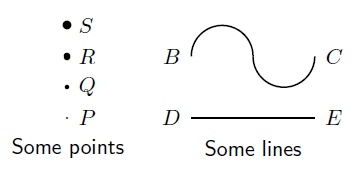
\includegraphics{col11306.imgs/m39370_MG10C13_001.png} % m39370;MG10C13\_001.png;;;6.0;8.5;
% \vspace{2pt}
% \vspace{\rubberspace}\par \begin{cnxcaption}
% \small \textbf{Figure 12.1: }Voorbeelde van ’n paar punte (aan gedui deur $P$, $Q$, $R$ en $S$) en ’n paar lyne (aan gedui deur $BC$ en $DE$).
% \end{cnxcaption}
% \vspace{.1in}
% \rule[.1in]{\figurerulewidth}{.005in} \\
% \end{center}
% \end{figure}       
% ’n Lyn word aangedui deur ’n beginpunt en ’n eindpunt. Ons noem ’n lyn wat begin by punt $A$ en eindig by punt $B$, $AB$. Aangsien die lyn van punt $B$ tot punt  $A$ dieselfde is as as die lyn van punt $A$ tot die punt  $B$, kan ons sê
% dat $AB=BA$.\par 
% When there is no ambiguity (which is the case throughout this text) Die lengte tussen die punte $A$ en $B$ is $AB$, the same as the notation to refer to the line itself. Dus as ons sê $AB=CD$ word dit bedoel dat die lengte van die
% lynstuk tussen $A$ en $B$ gelyk is aan die lengte tussen $C$ en $D$.
% \par 
% Note: in higher mathematics, where there might be some ambiguity between when we want refer to the length of the line and when we just want to refer to the line itself, the notation $|AB|$ is usually used to refer to the length of the line. In this case, if one says $|AB|=|CD|$, it means the lengths of the lines are the same, whereas if one says $AB=CD$, it means that the two lines actually coincide (i.e. they are the same). Throughout this text, however, this notation will not be used, and $AB=CD$ ALWAYS implies that the lengths are the same. \par A line is measured in units of length. Some common units of length are listed in Table 12.1.\par 
% % \textbf{m39370*uid8}\par
% \begin{table}[H]
% 
%  $ \hspace{-5pt}\begin{array}{cccccccccccc}   
\includegraphics[width=0.75cm]{col11306.imgs/summary_fullmarks.png} &   \end{array} $ \hspace{2 pt}\raisebox{-5 pt}{} {(section shortcode: MG10094 )} \par 
% able}[H]
% % \\ '' '0'
% \begin{center}
% 
% \begin{tabular}{|l|l|}\hline
%   \textbf{Eenheid van lengte}
%   &
%   \textbf{Afkorting}
% % make-rowspan-placeholders
% \\ \hline
% %--------------------------------------------------------------------
% kilometer &
% km% make-rowspan-placeholders
% \\ \hline
% %--------------------------------------------------------------------
% meter &
% m% make-rowspan-placeholders
% \\ \hline
% %--------------------------------------------------------------------
% sentimeter &
% cm% make-rowspan-placeholders
% \\ \hline
% %--------------------------------------------------------------------
% millimeter &
% mm% make-rowspan-placeholders
% \\ \hline
% %--------------------------------------------------------------------
% \end{tabular}
% \end{center}
% % \begin{center}{\small\bfseries Table 12.1}: Some common units of length and their abbreviations.\end{center}
% % \begin{caption}{\small\bfseries Table 12.1}:  ’n Paar algemene eenhede van lengte en hul afkortings.\end{caption}
% \end{table}
% \par
% 
\subsection*{Hoeke}

’n Hoek word gevorm as twee lyne in ’n gemeenskaplike punt ontmoet. Die punt waar twee lyne ontmoet staan bekend as die hoekpunt. Hoeke word aangedui deur ’n $\hat{}$ (genoem ’n kappie) bo ’n letter te plaas. Hoeke kan ook aangedui word met behulp van die lyn segmente waaruit die hoek bestaan, byvoorbeeld $C\hat{B}A$ of $A\hat{B}C$.

 Die $\angle $ simbool is 'n kort metode om hoek te skryf in meetkunde en word dikwels gebruik vir frases soos ``som van  $\angle$'e in 'n $\triangle$''. Hoeke word gemeet in grade wat aangedui word deur die simbool $^{\circ }$, 'n klein sirkeltjie bokant die teks soos 'n eksponent.\par 

% \Note{Hoeke kan ook gemeet word in radiale. In die hoërskool sal ons slegs grade gebruik, maar in wiskundige vakke op universiteitsvlak sal jy definitief weer radiale
% teëkom.}

\par 
\setcounter{subfigure}{0}
\setcounter{subfigure}{0}
\begin{figure}[H]
\begin{center}
\begin{pspicture}(0,-1.1732812)(3.1509376,1.1732812)
\psline[linewidth=0.04cm](0.2465625,-0.59328127)(2.7065625,0.94671875)
\psline[linewidth=0.04cm](0.2465625,-0.59328127)(2.8065624,-1.0132812)
\psarc[linewidth=0.04](0.8565625,-0.46328124){0.25}{289.65384}{82.874985}
% % \usefont{T1}{ptm}{m}{n}
\rput(2.9871874,-1.0232812){$A$}
% % \usefont{T1}{ptm}{m}{n}
\rput(2.871875,0.9767187){$C$}
% % \usefont{T1}{ptm}{m}{n}
\rput(0.0459375,-0.60328126){$B$}
\end{pspicture}
% \caption{Angle labelled as $\hat{B}$, $\angle CBA$ or $\angle ABC$}
\label{fig:mg:f:ma}
\end{center}
\end{figure}      
% \subsubsection{Meting van hoeke}
% \nopagebreak
% Die grootte van ’n hoek is onafhanklik van die lengtes van die twee sye wat die hoek onderspan. Dit hang slegs
% af van hoe die twee lyne relatief tot mekaar geplaas word, soos aangedui in Figuur 12.3. ’n Hoek vorm wanneer
% daar geroteer word om ’n hoekpunt.\par 
% 
% \subsubsection{Hoe om ’n gradeboog te gebruik}
% \nopagebreak
% ’n Gradeboog is ’n eenvoudige instrument wat gebruik word om hoeke te meet. ’n Diagram van ’n gradeboog
% word getoon in Figuur 12.4.\par 
% \setcounter{subfigure}{0}
% \begin{figure}[H] % horizontal\label{m39370*uid13}
% \begin{center}
% \rule[.1in]{\figurerulewidth}{.005in} \\
% \label{m39370*uid13!!!underscore!!!media}\label{m39370*uid13!!!underscore!!!printimage}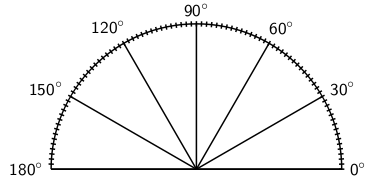
\includegraphics{col11306.imgs/m39370_MG10C13_004.png} % m39370;MG10C13\_004.png;;;6.0;8.5;
% \vspace{2pt}
% \vspace{\rubberspace}\par \begin{cnxcaption}
% \small \textbf{Figure 12.4: }Diagram van ’n gradeboog.
% \end{cnxcaption}
% \vspace{.1in}
% \rule[.1in]{\figurerulewidth}{.005in} \\
% \end{center}
% \end{figure}       
% 
% \textbf{Metode:}
% \par 
% Hoe om ’n gradeboog te gebruik:\par 
% \begin{enumerate}[noitemsep, label=\textbf{\arabic*}. ] 
% \item Plaas die onderste lyn van die gradeboog langs een van die sye van die hoek. Die tweede lyn moet in die
% rigting van die afgemete skaal wys.
% \item Beweeg die gradeboog sodat die middelpunt van die gradeboog en die hoekpunt oorstem.
% \item Lees af waar die tweede lyn van die hoek die afgemete skaal kruis. Maak seker dat jy by die 0$^{\circ }$ begin lees.
% \end{enumerate}
% 
% \subsubsection{ Meting van Hoeke: gebruik ’n gradeboog om die volgende hoeke te meet:}
% 
% 
% \setcounter{subfigure}{0}
% \begin{figure}[H] % horizontal\label{m39370*id314484}
% \begin{center}
% \label{m39370*id314484!!!underscore!!!media}\label{m39370*id314484!!!underscore!!!printimage}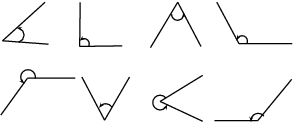
\includegraphics{col11306.imgs/m39370_MG10C13_005.png} % m39370;MG10C13\_005.png;;;6.0;8.5;
% \vspace{2pt}
% \vspace{.1in}
% \end{center}
% \end{figure}       
% \par 
% 
% \subsubsection{Spesiale Hoeke}
% \nopagebreak
% Wat is die kleinste hoek wat geteken kan word? Die figuur hier onder toon aan hoe twee lyne ($CA$ and $AB$)  ’n
% hoek onderspan by die hoekpunt $A$. As die lyn $CA$ geroteer word om die hoekpunt $A$, in die rigting van lyn $AB$, dan is die kleinste hoek wat geteken kan word, die geval waar beide lyne in dieselfde rigting wys. Dit noem ons ’n 0$^{\circ }$. Dit word aangedui in Figuur~12.6\par 
% 
% \setcounter{subfigure}{0}
% \begin{figure}[H] % horizontal\label{m39370*id314593}
% \begin{center}
% \label{m39370*id314593!!!underscore!!!media}\label{m39370*id314593!!!underscore!!!printimage}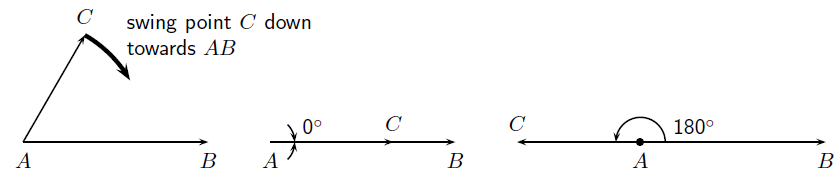
\includegraphics[width=.8\columnwidth]{col11306.imgs/m39370_MG10C13_006.png} % m39370;MG10C13\_006.png;;;6.0;8.5;
% \vspace{2pt}
% \vspace{.1in}
% \end{center}
% \end{figure}       
% \par 
% As lyn $CA$ nou opwaarts geroteer word, kan enige ander hoek gevorm word. As lyn $CA$ en lyn $AB$  in presies
% teenoorgestelde rigtings wys (soos in geval 3 in Figuur 12.6) dan word ’n 180$^{\circ }$ hoek onderspan.\par 
% 
% \Tip{As drie punte $A$, $B$ en $C$ op ’n reguitlyn lê, dan is die hoek wat onderspan word 180$^{\circ }$. Netso, as die hoek tussen 3 punte 180$^{\circ }$, is, dan lê die punte op ’n reguitlyn.}
% 
% \par
% ’n Hoek van 90$^{\circ }$  word ’n regte hoek genoem. ’n Regte hoek is die helfte van die hoek wat onderspan word deur
% die reguitlyn ( die 180$^{\circ }$ lyn). Ons sê dus $CA$ is loodreg op $AB$ of $CA\perp AB$.  ’n Hoek twee maal die grootte van
% die hoek wat die reguitlyn onderspan is 360$^{\circ }$. ’n Hoek van 360$^{\circ }$ is presies dieselfde as ’n 0$^{\circ }$, hoek (behalwe vir
% die notasie). Ons noem dit ’n omwenteling.\par 
% \setcounter{subfigure}{0}
% \begin{figure}[H] % horizontal\label{m39370*uid18}
% \begin{center}
% \rule[.1in]{\figurerulewidth}{.005in} \\
% \label{m39370*uid18!!!underscore!!!media}\label{m39370*uid18!!!underscore!!!printimage}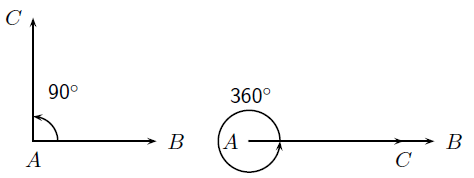
\includegraphics[width=.8\columnwidth]{col11306.imgs/m39370_MG10C13_007.png} % m39370;MG10C13\_007.png;;;6.0;8.5;
% \vspace{2pt}
% \vspace{\rubberspace}\par \begin{cnxcaption}
% \small \textbf{Figure 12.7: } ’n Hoek van 90$^{\circ }$ word aangedui as ’n regte hoek.
% \end{cnxcaption}
% \vspace{.1in}
% \rule[.1in]{\figurerulewidth}{.005in} \\
% \end{center}
% \end{figure}       
% 
% \subsubsection{Hoeke groter as 360$^{\circ }$ }
% \nopagebreak
% Alle hoeke groter as 360$^{\circ }$ lyk dieselfde as hoeke wat ons alreeds teëgekom het. As jy ’n hoek gegee word wat
% groter is as 360$^{\circ }$, trek 360$^{\circ }$ herhaaldelik af van die hoek, tot jy ’n antwoord kry tussen 0$^{\circ }$ en 360$^{\circ }$.Hoeke wat
% meer as 360$^{\circ }$ is meestal vir die wiskundige gerief. \par 
% 
% \Tip{
% \begin{itemize}[noitemsep]
% \item Skerphoek : ’n Hoek $\ge {0}^{\circ }$ and $<{90}^{\circ }$.
% \item Regtehoek : ’n Hoek gelyk aan ${90}^{\circ }$.
% \item Stomphoek : ’n Hoek $>{90}^{\circ }$ and $<{180}^{\circ }$.
% \item Reguitlynhoek : ’n Hoek gelyk aan 180$^{\circ }$.
% \item Inspringende hoek : $>{180}^{\circ }$ and $<{360}^{\circ }$.
% \item Omwenteling: ’n Hoek gelyk aan ${360}^{\circ }$.
% \end{itemize}
% Hierdie is basies net name vir hoeke in ‘n spesifieke reeks, soos gewys in Figuur ~12.8.}
% \par
% \setcounter{subfigure}{0}
% \begin{figure}[H] % horizontal\label{m39370*uid25}
% \begin{center}
% \rule[.1in]{\figurerulewidth}{.005in} \\
% \label{m39370*uid25!!!underscore!!!media}\label{m39370*uid25!!!underscore!!!printimage}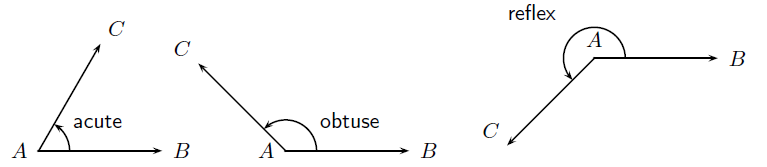
\includegraphics[width=.8\columnwidth]{col11306.imgs/m39370_MG10C13_008.png} % m39370;MG10C13\_008.png;;;6.0;8.5;
% \vspace{2pt}
% \vspace{\rubberspace}\par \begin{cnxcaption}
% \small \textbf{Figure 12.8: }Drie soorte hoeke.
% \end{cnxcaption}
% \vspace{.1in}
% \rule[.1in]{\figurerulewidth}{.005in} \\
% \end{center}
% \end{figure}       
% Waneer jy hoeke meet, kan jy hulle met mekaar vergelyk. Byvoorbeeld, alle regte hoeke is 90$^{\circ }$, dus is alle regte
% hoeke is gelyk aan mekaar en ‘n stomphoek sal altyd groter wees as ‘n skerphoek.\par Die volgende video gee ‘n opsomming van wat jy moet weet van hoeke.
% \setcounter{subfigure}{0}
% \begin{figure}[H] % horizontal\label{m39370*angles-1}
% \textnormal{Khan Academy video on angles - 1}\vspace{.1in} \nopagebreak
% \label{m39370*yt-media1}\label{m39370*yt-video1}
% \raisebox{-5 pt}{ 
\includegraphics[width=0.5cm]{col11306.imgs/summary_www.png}} { (Video:  MG10088 )}
% \vspace{2pt}
% \vspace{.1in}
% \end{figure}       
% Let daarop dat vir hoërskool sal jy net grade gebruik, nie radiale soos gewys in die video nie. Radiale is ‘n ander
% manier om hoeke te meet. Jy sal op universiteit aan radiale voorgestel word. \par 
% 
\subsection*{Eienskappe en notasie}

In die diagram hieronder, sny die twee reguitlyne $AB$ en $CD$ by punt $X$, om vier hoeke $\hat{a}$, $\hat{b}$, $\hat{c}$ en $\hat{d}$ te vorm.\par 
% Need new diagram here 
\setcounter{subfigure}{0}
 	\begin{figure}[H] 
    \begin{center}
\scalebox{1.2} % Change this value to rescale the drawing.
{
\begin{pspicture}(0,-1.124111)(4.2,1.124111)
\psline[linewidth=0.028222222cm,arrowsize=0.05291667cm 2.0,arrowlength=1.4,arrowinset=0.4]{<->}(0.08588889,-1.11)(4.145889,1.11)
\psline[linewidth=0.028222222cm,arrowsize=0.05291667cm 2.0,arrowlength=1.4,arrowinset=0.4]{<->}(0.0,0.9358889)(4.185889,-1.05)
\psarc[linewidth=0.028222222](2.1029444,-0.011166667){0.58294445}{330.0}{30.0}
\psarc[linewidth=0.028222222](1.9629444,-0.057055555){0.53705555}{150.0}{210.0}
\psarc[linewidth=0.028222222](2.0679445,-0.022055555){0.42205554}{30.0}{157.48302}
\psarc[linewidth=0.028222222](2.0579445,-0.012055555){0.47205555}{210.0}{330.0}
\psarc[linewidth=0.028222222](2.0629444,-0.037055556){0.49705556}{30.0}{155.69582}
\psarc[linewidth=0.028222222](2.0529444,-0.0070555555){0.54705554}{210.0}{330.0}
% % \usefont{T1}{ptm}{m}{n}
\rput(2.4014063,-0.004111111){\small{$a$}}
% % \usefont{T1}{ptm}{m}{n}
\rput(2.0214062,0.21588889){\small{$b$}}
% % \usefont{T1}{ptm}{m}{n}
\rput(1.7014062,-0.04411111){\small{$c$}}
% % \usefont{T1}{ptm}{m}{n}
\rput(2.1014063,-0.2841111){\small{$d$}}
\end{pspicture} 
}

    \end{center}
% \caption{Two intersecting straight lines with vertical angles $\hat{A},\hat{C}$ and $\hat{B},\hat{D}$.}
\label{fig:mg:f:specialangles2}
 \end{figure}        
Die volgende tabel gee ‘n opsomming van die spesiale hoekpare wat gevorm word as twee reguitlyne mekaar sny.\par 
% \textbf{m39370*id315548}\par

\begin{table}[H]
\begin{center}
\begin{tabular}{|p{3.5cm}|p{4cm}|p{4cm}|} \hline
\textbf{Term} & \textbf{Eienskap} & \textbf{Byvoorbeeld} \\ \hline
Skerphoek & $0^{\circ} < \mbox{hoek} < 90^{\circ}$ & $\hat{a}$; $\hat{c}$ \\ \hline
Regte hoek & Hoek $= 90^{\circ}$ &  \\ \hline
Stomphoek & $90^{\circ} < \mbox{hoek} < 180^{\circ}$ & $\hat{b}$; $\hat{d}$ \\ \hline
Gestrekte hoek & Hoek $= 180^{\circ}$ & $\hat{a} + \hat{b}$; $\hat{b} + \hat{c}$  \\ \hline
Inspringende hoek & $180^{\circ} < \mbox{hoek} < 360^{\circ}$ &  $\hat{a} + \hat{b} + \hat{c}$\\ \hline
Aangrensende hoeke & Hoeke wat 'n hoekpunt en 'n gemeenskaplike sy deel. & $\hat{a}$ en $\hat{d}$; $\hat{c}$ en $\hat{d}$ \\ \hline
Teenoorstaande of regoorstaande hoeke & Hoeke regoor mekaar wanneer twee lyne mekaar sny. Hulle deel 'n hoekpunt en is ewe groot. & $\hat{a}=\hat{c}$; $\hat{b}=\hat{d}$\\ \hline
Supplementêre hoeke & Hoeke waarvan die som $180^{\circ}$ is. & $\hat{a}+\hat{b}=180^{\circ}$; $\hat{b}+\hat{c}=180^{\circ}$ \\ \hline
Komplementêre hoeke  & Hoeke waarvan die som  $90^{\circ}$ is. & \\ \hline
Omwenteling & Som van al die hoeke om 'n punt. &  $\hat{a}+\hat{b}+\hat{c}+\hat{d}=360^{\circ}$ \\ \hline

\end{tabular}
\end{center}
\end{table}
 Let op dat aangrensende hoeke op ‘n reguitlyn supplementêr is.

% \Tip{Die teenoorstaande/regoorstaande hoeke wat gevorm word by twee snydende
% lyne is altyd ewe groot. 
% }


\subsection*{Ewewydige lyne en dwarslyne} Twee lyne sny mekaar as hulle kruis by ‘n punt. Byvoorbeeld, by ‘n verkeerskruising sny twee of meer strate en die snypunt van die kruising is die gemeenskaplike punt tussen die strate. Ewewydige lyne is lyne wat nooit kruis nie. Hulle word aangedui deur pyle, soos hieronder getoon is.
\par 
\setcounter{subfigure}{0}
\begin{figure}[H]
 \begin{center}
\scalebox{1}{
  \begin{pspicture}(0,0)(5,5)
%Lines MN and OP
\psline[linewidth=0.04cm](0,0)(5,3)
\psline[linewidth=0.01cm,arrowsize=0.2cm 2.0,arrowlength=1.4,arrowinset=0.5]{->}(2.3,1.4)(2.7,1.6)
\psline[linewidth=0.04cm](0.5,-.5)(5.5,2.5)
\psline[linewidth=0.01cm,arrowsize=0.2cm 2.0,arrowlength=1.4,arrowinset=0.5]{->}(2.5,0.7)(2.8,.9)
%Lines AB and CD
\psline[linewidth=0.04cm](2.5,-.5)(0.5,2.5)
\psline[linewidth=0.01cm,arrowsize=0.2cm 2.0,arrowlength=1.4,arrowinset=0.5]{->>}(2.5,-0.5)(2.2,0)
\psline[linewidth=0.04cm](5,0)(3,3)
\psline[linewidth=0.01cm,arrowsize=0.2cm 2.0,arrowlength=1.4,arrowinset=0.5]{->>}(4.6,0.6)(4.3,1.1)
%And the labels
\rput[t](0.5,2.8){$M$}
\rput[b](2.5,-.8){$N$}
\rput[b](5,-.3){$P$}
\rput[t](3,3.3){$O$}
\rput[l](-.3,0){$A$}
\rput[r](5.3,3){$B$}
\rput[l](0.2,-.5){$C$}
\rput[r](5.8,2.5){$D$}
  \end{pspicture}
}  
 \end{center}
\end{figure} 
%english
Ons gebruik twee vertikale lyne om aan te dui dat die twee lyne
ewewydig is:
\begin{equation*}
  AB \parallel CD \mbox{ en } MN \parallel OP
\end{equation*}
% \Note{’n Gedeelte van die Australiese Nasionale Spoorlyn is van die langste ewewydige
% lyne in die wêreld..
% (Source: www.guinnessworldrecords.com) Die Australian National Railways Trans-
% Australian lyn oor die Nullarbor vlakte, is 478 km (297 myle) pylreguit,
% van Myl 496, tussen Nurina en Loongana, Western Australia, tot by
% Myl 793, tussen Ooldea en Watson, South Australia.}
     
’n Dwarslyn van twee of meer lyne is ‘n lyn wat hierdie lyne sny. In die figuur hieronder, $AB \parallel CD$ en $EF$ is ‘n dwarslyn. \par 
\setcounter{subfigure}{0}
\begin{figure}[htb]
\begin{center}
\begin{pspicture}(0,-1.5)(6,3.5)
%\psgrid[gridcolor=lightgray]
\psline{-}(0,0)(6,0)
\psline[linewidth=0.01cm,arrowsize=0.2cm 2.0,arrowlength=1.4,arrowinset=0.5]{->}(0,0)(1.5,0)
\uput[l](0,0){$A$}
\uput[r](6,0){$B$}
\psline{-}(0,2)(6,2)
\psline[linewidth=0.01cm,arrowsize=0.2cm 2.0,arrowlength=1.4,arrowinset=0.5]{->}(0,2)(1.5,2)
\uput[l](0,2){$C$}
\uput[r](6,2){$D$}
\psline{-}(1,-1)(5,3)
\uput[dl](1,-1){$E$}
\uput[ur](5,3){$F$}

\psarc(4,2){0.5}{0}{45} \uput{0.6}[22.5](4,2){$g$}
\psarc(4,2){0.3}{45}{180} \psarc(4,2){0.4}{45}{180} \uput{0.5}[112.5](4,2){$h$}
\psarc(4,2){0.5}{180}{225} \uput{0.6}[202.5](4,2){$a$}
\psarc(4,2){0.3}{225}{360} \psarc(4,2){0.4}{225}{360} \uput{0.5}[292.5](4,2){$b$}
\psarc(2,0){0.5}{0}{45} \uput{0.6}[22.5](2,0){$c$}
\psarc(2,0){0.3}{45}{180} \psarc(2,0){0.4}{45}{180} \uput{0.5}[112.5](2,0){$d$}
\psarc(2,0){0.5}{180}{225} \uput{0.6}[202.5](2,0){$e$}
\psarc(2,0){0.3}{225}{360} \psarc(2,0){0.4}{225}{360} \uput{0.5}[292.5](2,0){$f$}
\end{pspicture}
% \caption{Parallel lines intersected by a transversal}
\label{fig:mg:f:partrans}
\end{center}
\end{figure}      
Die eienskappe van hoeke wat gevorm word by hierdie
kruisende lyne word opgesom in die volgende tabel:
\begin{table}[H]
\begin{center}
%\caption{Properties of angles formed when parallel lines are intersected by a transversal. The example in Figure~\ref{fig:mg:f:partrans} is used as a reference.}
\label{tab:mg:f:partrans}
\begin{tabular}{|p{2.75cm}|p{4cm}|p{3cm}|p{2.5cm}|}\hline
\textbf{Naam van hoeke} & \textbf{Definisie} & \textbf{Byvoorbeeld} & \textbf{Notas}\\\hline
Binnehoeke & Hoeke wat binne die ewewydige lyne lê  & $\hat{a}$, $\hat{b}$, $\hat{c}$ en $\hat{d}$ is binnehoeke & Die woord binnehoeke beteken ``tussen die lyne'' \\ \hline
Buitehoeke & Hoeke wat buite die ewewydige lyne lê & $\hat{e}$, $\hat{f}$, $\hat{g}$ en $\hat{h}$ is buitehoeke & Die woord buitehoeke beteken ``aan die buitekant'' \\ \hline
Ooreenkomstige hoeke & Die hoeke aan dieselfde kant van die snylyn en aan dieselfde kant van die lyne. As die lyne ewewydige is, is die ooreenkomstige hoeke gelyk. & $\hat{a}$ en $\hat{e}$,  $\hat{b}$ en $\hat{f}$,  $\hat{c}$ en $\hat{g}$,   $\hat{d}$ en $\hat{h}$ is pare ooreenkomstige hoeke:  $\hat{a} = \hat{e}$, $\hat{b} = \hat{f}$, $\hat{c} = \hat{g}$ en  $\hat{d} = \hat{h}$. &
\raisebox{-.8\height}{
%\scalebox{1} % Change this value to rescale the drawing.
% \begin{center}
%{
\begin{pspicture}(0,-0.9884375)(1.48,0.7884375)
\psline[linewidth=0.04cm](0.2,0.7684375)(1.46,0.7684375)
\psline[linewidth=0.04cm](0.22,0.1284375)(1.44,0.1284375)
\psline[linewidth=0.01cm,arrowsize=0.2cm 2.0,arrowlength=1.4,arrowinset=0.5]{->>}(0.38,0.1284375)(1.16,0.1284375)
\psline[linewidth=0.01cm,arrowsize=0.2cm 2.0,arrowlength=1.4,arrowinset=0.5]{->>}(0.22,0.7684375)(1.0,0.7684375)
% % \usefont{T1}{ptm}{m}{n}
\rput(0.7128125,-0.7615625){F vorm}
\psline[linewidth=0.04cm](0.2,0.7684375)(0.2,-0.5315625)
\psarc[linewidth=0.04](0.2,0.7484375){0.2}{270.0}{0.0}
\psarc[linewidth=0.04](0.22,0.1084375){0.2}{270.0}{0.0}
\end{pspicture} }
%}
% \end{center}
\\\hline
Ko-binnehoeke  & Ko-binnehoeke wat aan dieselfde kant van die snylyn lê. As die lyne ewewydig is, is die ko-binnehoeke gelyk. &  $\hat{a}$ en $ \hat{d}$, $\hat{b}$ en $\hat{c}$ is ko-binnehoeke. $\hat{a} + \hat{d} = 180^{\circ}$, $\hat{b} + \hat{c} = 180^{\circ}$.&
% \begin{center}
\raisebox{-.8\height}{
%\scalebox{1} % Change this value to rescale the drawing.
%{
\begin{pspicture}(0,-0.8384375)(1.64,0.6513173)
\psline[linewidth=0.04cm](0.24,0.6184375)(1.5,0.6184375)
\psline[linewidth=0.04cm](0.26,-0.3415625)(1.62,-0.3415625)
\psline[linewidth=0.01cm,arrowsize=0.2cm 2.0,arrowlength=1.4,arrowinset=0.5]{->>}(0.42,-0.3415625)(1.2,-0.3415625)
\psline[linewidth=0.01cm,arrowsize=0.2cm 2.0,arrowlength=1.4,arrowinset=0.5]{->>}(0.26,0.6184375)(1.04,0.6184375)
\psarc[linewidth=0.04](0.24,-0.3815625){0.24}{7.125016}{90.0}
% % \usefont{T1}{ptm}{m}{n}
\rput(0.83671874,-0.8){C vorm}
\psline[linewidth=0.04cm](0.24,0.6184375)(0.24,-0.3615625)
\psarc[linewidth=0.04](0.24,0.5984375){0.2}{270.0}{9.462322}
\end{pspicture} }
%}
% \end{center}
\\\hline
Verwisselende binnehoeke & Die binnehoeke wat aan verskillende kante van die snylyn lê. As die lyne ewewydige is, is die verwisselende hoeke ewe groot. & $\hat{a}$ en $\hat{c}$, $\hat{b} $ en $\hat{d}$ is pare verwisselende binnehoeke: $\hat{a} = \hat{c}$, $\hat{b} = \hat{d}$.&
% \begin{center}
\raisebox{-.8\height}{
%\scalebox{1} % Change this value to rescale the drawing.
%{
\begin{pspicture}(0,-0.8184375)(1.4,0.6584375)
\psline[linewidth=0.04cm](0.0,0.6384375)(1.26,0.6384375)
\psline[linewidth=0.04cm](1.26,0.6384375)(0.02,-0.3215625)
\psline[linewidth=0.04cm](0.02,-0.3215625)(1.38,-0.3215625)
\psline[linewidth=0.01cm,arrowsize=0.2cm 2.0,arrowlength=1.4,arrowinset=0.5]{->>}(0.18,-0.3215625)(0.96,-0.3215625)
\psline[linewidth=0.01cm,arrowsize=0.2cm 2.0,arrowlength=1.4,arrowinset=0.5]{->>}(0.02,0.6384375)(0.8,0.6384375)
\psarc[linewidth=0.04](1.06,0.5784375){0.2}{168.69006}{243.43495}
\psarc[linewidth=0.04](0.2465625,-0.215){0.2265625}{329.03625}{45.0}
% % \usefont{T1}{ptm}{m}{n}
\rput(0.591875,-0.8){Z vorm}
\end{pspicture} }
%}
% \end{center}
\\\hline
\end{tabular}
\end{center}
\end{table}

As twee ewewydige lyne gesny word met ’n dwarslyn, sodat:
\begin{itemize}[noitemsep]
 \item ooreenkomstige hoeke gelyk is; of
\item verwisselende binnehoeke gelyk is; of
\item ko-binnehoeke aan dieselfde kant van die snylyn supplementêr is
\end{itemize}
dan is die twee lyne ewewydig.

\clearpage

% \pagebreak %MANUAL PGBREAK TO FORCE WEX BELOW TO SPLIT (still doesnt split properly. Damn mdframed!!!)
\begin{wex}{Berekening van hoeke}
{Vind al die onbekende hoeke in die volgende figure. Is $EF \parallel CG$? Verduidelik jou antwoord.
 \begin{center}
   \scalebox{0.8} % Change this value to rescale the drawing.
{
\begin{pspicture}(0,-2.57375)(12.675937,2.57375)
\psline[linewidth=0.01cm,arrowsize=0.2cm 2.0,arrowlength=1.4,arrowinset=0.5]{->}(3.68,0.07124995)(4.32,0.43124995)
\psline[linewidth=0.01cm,arrowsize=0.2cm 2.0,arrowlength=1.4,arrowinset=0.5]{->}(8.18,-0.18875004)(8.8,0.17124996)
\rput{-143.0545}(8.17638,3.9190145){\psarc[linewidth=0.04](4.742796,0.5937799){0.49404234}{343.58032}{85.22324}}
\psline[linewidth=0.04cm](0.0,-2.14875)(6.62,1.83125)
\psline[linewidth=0.04cm](4.96,-2.12875)(12.14,2.23375)
\psline[linewidth=0.04cm](2.96,-2.10875)(9.0,-2.10875)
\psline[linewidth=0.04cm](4.96,-2.10875)(5.0,0.89124984)
\psline[linewidth=0.04cm](2.44,-0.64875007)(12.48,1.53375)
\psline[linewidth=0.04cm](4.8,-2.0887501)(4.8,-1.96875)
\psline[linewidth=0.04cm](4.78,-1.94875)(4.98,-1.94875)
% \usefont{T1}{ptm}{m}{n}
\rput(4.7,0.44624996){\footnotesize $60^{\circ}$}
\psbezier[linewidth=0.04](1.94,-1.0062499)(2.46,-1.52625)(3.24,-1.02625)(3.18,-0.52624995)
% \usefont{T1}{ptm}{m}{n}
\rput{0.86235595}(-0.013302135,-0.039991397){\rput(2.623804,-0.9042548){\footnotesize $160^{\circ}$}}
\psarc[linewidth=0.04](5.09,-1.7787501){0.39}{351.02737}{104.74356}
\rput{-33.527527}(1.9972864,2.8241615){\psarc[linewidth=0.04](5.6863933,-1.9031615){0.33947578}{0.0}{99.46232}}
\rput{-210.4531}(17.459091,-3.5844944){\psarc[linewidth=0.04](9.217381,0.58386225){0.3534083}{0.0}{78.96434}}
\rput{-28.674759}(0.6394295,5.5710244){\psarc[linewidth=0.04](11.218004,1.5346314){0.32564545}{343.67474}{75.4531}}
\psbezier[linewidth=0.04](9.8,0.7850357)(10.352,0.33375004)(10.9,0.71375006)(10.96,1.21375)
% \usefont{T1}{ptm}{m}{n}
\rput(5.1759377,-1.67875){$x$}
% \usefont{T1}{ptm}{m}{n}
\rput(5.6659374,-1.8987501){$s$}
% \usefont{T1}{ptm}{m}{n}
\rput(9.165937,0.66124994){$y$}
% \usefont{T1}{ptm}{m}{n}
\rput(10.395937,0.88124996){$r$}
% \usefont{T1}{ptm}{m}{n}
\rput(11.285938,1.5012499){$p$}
% \usefont{T1}{ptm}{m}{n}
\rput(4.862969,-2.41875){$C$}
% \usefont{T1}{ptm}{m}{n}
\rput(9.175625,-2.27875){$G$}
% \usefont{T1}{ptm}{m}{n}
\rput(12.290313,2.3812501){$D$}
% \usefont{T1}{ptm}{m}{n}
\rput(12.525156,1.34125){$F$}
% \usefont{T1}{ptm}{m}{n}
\rput(0.186875,-2.3387501){$A$}
% \usefont{T1}{ptm}{m}{n}
\rput(2.3165624,-0.35875005){$E$}
% \usefont{T1}{ptm}{m}{n}
\rput(4.8403125,1.18125){$B$}
\end{pspicture} 
 
}
 \end{center}
} 
{\westep{Gebruik eienskappe van ewewydige lyne om alle gelyke hoeke op die diagram te identifiseer}

\westep{Vind al die onbekende hoeke}
\begin{equation*}
\begin{array}{r@{\;}l@{\quad}l}
AB &\parallel CD & \mbox{(gegee)} \\
\therefore \hat{x}&=60^{\circ} & \mbox{(verwisselende binne $\angle$'e)}  \vspace{10pt} \\

\hat{y} + 160^\circ &= 180^{\circ}  & \mbox{(ko-binne $\angle$'e)} \\
\therefore \hat{y} &= 20^{\circ} &   \vspace{8pt}\\


\hat{p} &= \hat{y} & \mbox{(regoorstaande $\angle$'e)} \\
\therefore \hat{p} &= 20^{\circ} &  \vspace{10pt}\\



 \hat{r} + \hat{p} &= 180^{\circ}  &\mbox{ (som van $\angle$'e op 'n reguitlyn)} \\
\therefore \hat{r} &= 160^{\circ} &  \vspace{10pt}\\

\end{array}
\end{equation*} 
\begin{equation*}
\begin{array}{r@{\;}l@{\quad}l}
 \hat{s} + \hat{x} &= 90^{\circ}  & \mbox{(komplementêre $\angle$'e)} \\ 
 \hat{s} + 60^\circ &= 90^{\circ} & \\
\therefore \hat{s} &= 30^{\circ} &  
\end{array}
\end{equation*} 
\westep{Bewys of $EF \parallel CG$}
Indien $EF \parallel CG$ dan sal $\hat{p}$ gelyk aan ooreenkomstige hoek $\hat{s}$ wees, maar $\hat{p} = 20^{\circ}$ en
$\hat{s}= 30^{\circ}$. Dus $EF$ is nie ewewydig aan $ CG$ nie.

}
\end{wex}


\begin{exercises}{}
{
        \nopagebreak \noindent
\begin{enumerate}[label=\textbf{\arabic*}.]
\item Gebruik aangrensende, ooreenkomstige, verwisselende en ko-binnehoeke om al die hoeke wat met letters benoem is in die diagram hieronder, te vind:\\
\begin{pspicture}(0,-1.7981373)(6.5116725,1.7981373)
\psline[linewidth=0.04cm](0.34542254,0.6181373)(5.2654223,0.6181373)
\psline[linewidth=0.04cm](0.34542254,-0.7418627)(5.2654223,-0.7418627)
\psline[linewidth=0.04cm](0.0,-1.7781373)(5.5254226,1.7781373)
% % \usefont{T1}{ptm}{m}{n}
\rput(4.4,0.8){\footnotesize$42^\circ$}
% % \usefont{T1}{ptm}{m}{n}
\rput(3.664485,0.8881373){$a$}
% \usefont{T1}{ptm}{m}{n}
\rput(3.0458913,0.3881373){$b$}
% \usefont{T1}{ptm}{m}{n}
\rput(3.8072975,0.4081373){$c$}
% \usefont{T1}{ptm}{m}{n}
\rput(1.5262038,-0.5518627){$d$}
% \usefont{T1}{ptm}{m}{n}
\rput(2.2315164,-0.5518627){$e$}
% \usefont{T1}{ptm}{m}{n}
\rput(1.6212038,-1.0518627){$f$}
% \usefont{T1}{ptm}{m}{n}
\rput(1.05,-0.95){$g$}
\rput{-66.70425}(1.9155159,4.522671){\psarc[linewidth=0.032]{-}(4.3934965,0.8061751){0.24084859}{20.012312}{156.69316}}
\psline[linewidth=0.04](3.9254224,-0.6018627)(4.2254224,-0.7418627)(3.9454224,-0.8818627)
\psline[linewidth=0.04](3.6854224,-0.6018627)(3.9854226,-0.7418627)(3.7054226,-0.8818627)
\psline[linewidth=0.04](2.2454226,0.7581373)(2.5454226,0.6181373)(2.2654226,0.47813728)
\psline[linewidth=0.04](2.0054226,0.7581373)(2.3054225,0.6181373)(2.0254226,0.47813728)
\end{pspicture}
\\
\item Vind al die onbekende hoeke in die figuur hieronder: \\
\\
\scalebox{1.3} {
\begin{pspicture}(0,-1.6967187)(5.5376563,1.7167188)
\psline[linewidth=0.04cm](3.1065626,1.4032813)(5.0465627,-1.4567187)
\psline[linewidth=0.04cm](0.4665625,1.1832813)(2.4065626,-1.6767187)
\psline[linewidth=0.01cm,arrowsize=0.2cm 2.0,arrowlength=1.4,arrowinset=0.5]{->>}(0.49,1.1417187)(1.3465625,-0.11671878)
\psline[linewidth=0.01cm,arrowsize=0.2cm 2.0,arrowlength=1.4,arrowinset=0.5]{->>}(3.3065624,1.1032813)(4.29,-0.29828128)
\psline[linewidth=0.04cm](1.5065625,-0.3367187)(4.4465623,-0.5567187)
\psline[linewidth=0.04cm](0.8665625,0.6232813)(3.8065624,0.40328127)
\psline[linewidth=0.01cm,arrowsize=0.2cm 2.0,arrowlength=1.4,arrowinset=0.5]{->}(1.5265626,-0.33671877)(3.1265626,-0.47671878)
\psline[linewidth=0.01cm,arrowsize=0.2cm 2.0,arrowlength=1.4,arrowinset=0.5]{->}(1.0065625,0.62328136)(2.77,0.48171872)
\psline[linewidth=0.04cm](3.7665625,0.40328127)(1.5065625,-0.3367187)
\psline[linewidth=0.04cm](4.4065623,-0.5567187)(2.1465626,-1.2967187)
\psline[linewidth=0.01cm,arrowsize=0.2cm 2.0,arrowlength=1.4,arrowinset=0.5]{->}(3.2065625,0.22328123)(2.3665626,-0.09671878)
\psline[linewidth=0.01cm,arrowsize=0.2cm 2.0,arrowlength=1.4,arrowinset=0.5]{->}(3.4065626,0.30328122)(2.5665624,-0.01671878)
\psline[linewidth=0.01cm,arrowsize=0.2cm 2.0,arrowlength=1.4,arrowinset=0.5]{->}(3.6265626,0.38328123)(2.7865624,0.06328122)
\psline[linewidth=0.01cm,arrowsize=0.2cm 2.0,arrowlength=1.4,arrowinset=0.5]{->}(3.7465625,-0.7767188)(2.89,-1.0782813)
\psline[linewidth=0.01cm,arrowsize=0.2cm 2.0,arrowlength=1.4,arrowinset=0.5]{->}(3.9465625,-0.69671875)(3.1065626,-1.0167189)
\psline[linewidth=0.01cm,arrowsize=0.2cm 2.0,arrowlength=1.4,arrowinset=0.5]{->}(4.1665626,-0.61671877)(3.3265624,-0.93671876)
\usefont{T1}{ptm}{m}{n}
\rput(0.28453124,1.1932813){$A$}
\usefont{T1}{ptm}{m}{n}
\rput(0.60765624,0.5132813){$B$}
\usefont{T1}{ptm}{m}{n}
\rput(1.3045312,-0.54627085){$C$}
\usefont{T1}{ptm}{m}{n}
\rput(1.9399999,-1.3867188){$D$}
\usefont{T1}{ptm}{m}{n}
\rput(3.2096875,1.5132812){$E$}
\usefont{T1}{ptm}{m}{n}
\rput(4.1,0.49328125){$F$}
\usefont{T1}{ptm}{m}{n}
\rput(4.7,-0.46671876){$G$}
\usefont{T1}{ptm}{m}{n}
\rput(5.1331253,-1.3267187){$H$}
\usefont{T1}{ptm}{m}{n}
\rput(1.25,0.46){\tiny $70^\circ$}
\usefont{T1}{ptm}{m}{n}
\rput(2.3,-1.0917187){\tiny $80^\circ$}
\usefont{T1}{ptm}{m}{n}
\rput(0.87921876,0.7532813){\tiny $1$}
\usefont{T1}{ptm}{m}{n}
\rput(3.4192188,0.61328125){\tiny $1$}
\usefont{T1}{ptm}{m}{n}
\rput(3.144219,0.33328128){\tiny $2$}
\usefont{T1}{ptm}{m}{n}
\rput(3.6359375,0.21328127){\tiny $3$}
\usefont{T1}{ptm}{m}{n}
\rput(4.119219,-0.4){\tiny $1$}
\usefont{T1}{ptm}{m}{n}
\rput(3.7442188,-0.6667187){\tiny $2$}
\usefont{T1}{ptm}{m}{n}
\rput(4.2959375,-0.7467187){\tiny $3$}
\usefont{T1}{ptm}{m}{n}
\rput(1.5392189,-0.09){\tiny $1$}
\usefont{T1}{ptm}{m}{n}
\rput(2.1442187,-0.28671873){\tiny $2$}
\usefont{T1}{ptm}{m}{n}
\rput(1.7959374,-0.5667187){\tiny $3$}
\usefont{T1}{ptm}{m}{n}
\rput(2.3192186,-1.3667188){\tiny $1$}
\rput{-165.35927}(1.9916399,1.1648247){\psarc[linewidth=0.04](1.0706391,0.4544851){0.34608197}{92.73279}{185.53572}}
\rput{-45.10457}(1.5105618,1.2407944){\psarc[linewidth=0.04](2.2491949,-1.1983162){0.29357287}{50.13503}{194.957}}
\end{pspicture}
}  \\ 
\item Vind die waarde van $x$ in die figuur hieronder: \\
\scalebox{1.3} 
{
\begin{pspicture}(0,-2.203125)(2.966696,2.203125)
\psline[linewidth=0.04cm](0.636875,1.8096874)(0.636875,-1.7303125)
\psline[linewidth=0.04cm](1.636875,1.8096874)(1.636875,-1.7303125)
\psline[linewidth=0.04cm](0.396875,1.0096875)(2.72,-1.116875)
\psline[linewidth=0.04cm](1.876875,0.18968745)(0.476875,-1.6903126)
\usefont{T1}{ptm}{m}{n}
\rput(0.63859373,1.9996876){$A$}
\usefont{T1}{ptm}{m}{n}
\rput(0.59796876,-2.0003126){$B$}
\usefont{T1}{ptm}{m}{n}
\rput(1.6039063,-2.0003126){$C$}
\usefont{T1}{ptm}{m}{n}
\rput(1.6103125,1.9996876){$D$}
\usefont{T1}{ptm}{m}{n}
\rput(0.29453126,0.67968744){$X$}
\usefont{T1}{ptm}{m}{n}
\rput(1.4804688,-0.7010938){$Y$}
\usefont{T1}{ptm}{m}{n}
\rput(0.41609374,-1.3803126){$Z$}
\psline[linewidth=0.04cm](0.616875,1.4496874)(0.736875,1.6896874)
\psline[linewidth=0.04cm](0.616875,1.5096875)(0.536875,1.6896874)
\psline[linewidth=0.04cm](1.636875,1.5496875)(1.736875,1.7296875)
\psline[linewidth=0.04cm](1.636875,1.5496875)(1.536875,1.7096874)
\usefont{T1}{ptm}{m}{n}
\rput(0.8385938,0.33468747){\scriptsize $4x$}
\usefont{T1}{ptm}{m}{n}
\rput(1.8557812,-0.10531255){\scriptsize $x$}
\usefont{T1}{ptm}{m}{n}
\rput{-40.134434}(1.2350872,1.2198397){\rput(2.2690625,-1.0780938){\scriptsize $x+20^\circ$}}
\rput{-178.50352}(3.4745831,-0.6899131){\psarc[linewidth=0.04](1.7327864,-0.36764556){0.17893833}{61.938473}{168.11142}}
\end{pspicture} 
} \\
\item Bepaal of daar pare ewewydige lyne is in die volgende figure:
\begin{enumerate}[itemsep=10pt, label=\textbf{(\alph*)} ] 
            \item 
\scalebox{1} % Change this value to rescale the drawing.
{
\begin{pspicture}(0,-2.451875)(6.3617187,2.451875)
\psline[linewidth=0.04cm](0.0,1.6081251)(6.1,-1.751875)
\psline[linewidth=0.04cm](1.42,2.171875)(1.74,-1.808125)
\psline[linewidth=0.04cm](4.72,2.188125)(5.08,-2.211875)
% \usefont{T1}{ptm}{m}{n}
\rput(2,0.85812503){$115^{\circ}$}
% \usefont{T1}{ptm}{m}{n}
\rput(4.583125,-0.621875){$55^{\circ}$}
% \usefont{T1}{ptm}{m}{n}
\rput(1.2482814,2.278125){$O$}
% \usefont{T1}{ptm}{m}{n}
\rput(1.5804688,-2.021875){$P$}
% \usefont{T1}{ptm}{m}{n}
\rput(4.9214063,2.178125){$Q$}
% \usefont{T1}{ptm}{m}{n}
\rput(5.2339063,-2.301875){$R$}
% \usefont{T1}{ptm}{m}{n}
\rput(0.3,1.678125){$S$}
% \usefont{T1}{ptm}{m}{n}
\rput(6.210781,-1.7818749){$T$}
% \usefont{T1}{ptm}{m}{n}
\rput(1.3671875,0.21812505){$A$}
% \usefont{T1}{ptm}{m}{n}
\rput(4.5465627,-1.361875){$B$}
% \usefont{T1}{ptm}{m}{n}
\rput(1.3509375,0.97812504){\tiny $1$}
% \usefont{T1}{ptm}{m}{n}
\rput(1.3359375,0.65812504){\tiny $2$}
% \usefont{T1}{ptm}{m}{n}
\rput(1.6876563,0.51812506){\tiny $3$}
% \usefont{T1}{ptm}{m}{n}
\rput(5.1876564,-1.5218749){\tiny $3$}
% \usefont{T1}{ptm}{m}{n}
\rput(5.215937,-1.0618749){\tiny $2$}
% \usefont{T1}{ptm}{m}{n}
\rput(4.8,-1.3018749){\tiny $1$}
\end{pspicture} 
}
\\
\item 
\scalebox{1} % Change this value to rescale the drawing.
{
\begin{pspicture}(0,-2.8392186)(7.70125,2.8392186)
\psline[linewidth=0.04cm](0.0625,-0.05921875)(7.4625,-0.05921875)
\psline[linewidth=0.04cm](0.6625,-1.9592187)(4.74,2.5192187)
\psline[linewidth=0.04cm](6.1225,2.4007812)(2.0025,-2.6592188)
% \usefont{T1}{ptm}{m}{n}
\rput(4.8440623,0.25078127){$45^{\circ}$}
% \usefont{T1}{ptm}{m}{n}
\rput(2.5667188,-0.28921875){$124^{\circ}$}
% \usefont{T1}{ptm}{m}{n}
\rput(4.7973437,2.6707811){$M$}
% \usefont{T1}{ptm}{m}{n}
\rput(0.601875,-1.7292187){$N$}
% \usefont{T1}{ptm}{m}{n}
\rput(6.250781,2.4707813){$O$}
% \usefont{T1}{ptm}{m}{n}
\rput(2.2229688,-2.6892188){$P$}
% \usefont{T1}{ptm}{m}{n}
\rput(0.10390625,0.19078125){$Q$}
% \usefont{T1}{ptm}{m}{n}
\rput(7.536406,0.13078125){$R$}
% \usefont{T1}{ptm}{m}{n}
\rput(2.21875,0.49078128){$K$}
% \usefont{T1}{ptm}{m}{n}
\rput(4.4520316,-0.5492188){$L$}
% \usefont{T1}{ptm}{m}{n}
\rput(2.3734376,0.13078125){\tiny $1$}
% \usefont{T1}{ptm}{m}{n}
\rput(2.7584374,0.09078125){\tiny $2$}
% \usefont{T1}{ptm}{m}{n}
\rput(2.0901563,-0.18921876){\tiny $3$}
% \usefont{T1}{ptm}{m}{n}
\rput(4.170156,-0.28921875){\tiny $3$}
% \usefont{T1}{ptm}{m}{n}
\rput(4.0184374,0.09078125){\tiny $2$}
% \usefont{T1}{ptm}{m}{n}
\rput(3.7334375,-0.22921875){\tiny $1$}
\end{pspicture} 
}
    \item 
\scalebox{1} % Change this value to rescale the drawing.
{
\begin{pspicture}(0,-3.1192186)(6.325469,3.1192186)
\psline[linewidth=0.04cm](0.1525,1.0007812)(6.1125,0.98078126)
\psline[linewidth=0.04cm](0.1525,-1.0392187)(6.1125,-1.0192188)
\psline[linewidth=0.04cm](3.0125,3.0007813)(3.3125,-3.0192187)
% \usefont{T1}{ptm}{m}{n}
\rput(2.7432813,0.7307812){$95^{\circ}$}
% \usefont{T1}{ptm}{m}{n}
\rput(3.6395311,-1.3692188){$85^{\circ}$}
% \usefont{T1}{ptm}{m}{n}
\rput(3.24875,2.950781){$K$}
% \usefont{T1}{ptm}{m}{n}
\rput(3.5020313,-2.9692187){$L$}
% \usefont{T1}{ptm}{m}{n}
\rput(0.14734375,-0.88921875){$M$}
% \usefont{T1}{ptm}{m}{n}
\rput(6.0718746,-0.82921875){$N$}
% \usefont{T1}{ptm}{m}{n}
\rput(0.12328125,1.1707813){$T$}
% \usefont{T1}{ptm}{m}{n}
\rput(6.1564064,1.1507812){$Y$}
% \usefont{T1}{ptm}{m}{n}
\rput(3.3034375,0.79078126){\tiny $1$}
% \usefont{T1}{ptm}{m}{n}
\rput(3.3084376,1.2107813){\tiny $2$}
% \usefont{T1}{ptm}{m}{n}
\rput(2.9001563,1.1907812){\tiny $3$}
% \usefont{T1}{ptm}{m}{n}
\rput(3.3234375,-0.88921875){\tiny $1$}
% \usefont{T1}{ptm}{m}{n}
\rput(2.9884377,-0.88921875){\tiny $2$}
% \usefont{T1}{ptm}{m}{n}
\rput(3.0201561,-1.2692188){\tiny $3$}
\end{pspicture} 
}
    \end{enumerate}
\item As $AB$ ewewydig is aan $CD$ en $AB$ ewewydig is aan $EF$, bewys dat  $CD$ ewewydig is aan $EF$.\vspace{8pt}\\
\begin{pspicture}(0,-0.81328124)(3.8328125,0.81328124)
\psline[linewidth=0.04cm](0.2415625,0.6067188)(3.4415624,0.38671875)
\psline[linewidth=0.04cm](0.3015625,-0.09328125)(3.4215624,-0.09328125)
\psline[linewidth=0.04cm](0.3815625,-0.6532813)(3.5215626,-0.55328125)
\rput(0.1221875,-0.10328125){$A$}
\rput(3.6009376,-0.08328125){$B$}
\rput(3.654375,-0.5832813){$F$}
\rput(0.178125,-0.66328126){$E$}
\rput(0.086875,0.61671877){$C$}
\rput(3.6504688,0.33671874){$D$}
\end{pspicture}  
\end{enumerate}

% Automatically inserted shortcodes - number to insert 5
\par \practiceinfo
\par \begin{tabular}[h]{cccccc}
% Question 1
(1.)	02n7	&
% Question 2
(2.)	02n8	&
% Question 3
(3.)	02n9	&
% Question 4
(4.)	02na	&
% Question 5
(5.)	02nb	&
\end{tabular}
% Automatically inserted shortcodes - number inserted 5
}
\end{exercises}
\\
\\


        \subsection*{Klassifikasie van driehoeke}
'n Driehoek is ’n driesydige veelhoek. Driehoeke kan geklassifiseer word volgens sye of volgens hoeke: ongelyksydig, gelyksydig, gelykbenig, reghoekig, skerphoekig, stomphoekig. \par 

As die hoekpunte van ’n driehoek benoem word met $A$, $B$, en $C$, dan praat ons van $\triangle ABC$. \par 

\mindsetvid{Geometry toolkit}{VMciu}

\begin{table}[H]
\begin{center}
% \caption{Types of Triangles}
\label{tab:gt:basics:triangles}
\begin{tabular}{|l|m{3.8cm}|m{5cm}|}\hline
\textbf{Naam} & \textbf{Diagram} & \textbf{Eienskappe}\\\hline
Ongelyksydig &
\begin{center}
\scalebox{0.7}{
\begin{pspicture}(0,-1.531875)(1.3471875,1.531875)
% % \usefont{T1}{ptm}{m}{n}
\rput(0.8534375,1.358125){$A$}
% % \usefont{T1}{ptm}{m}{n}
\rput(1.1940625,-1.381875){$B$}
% % \usefont{T1}{ptm}{m}{n}
\rput(0.0940625,-0.361875){$C$}
\pspolygon[linewidth=0.04](0.326875,-0.31260228)(0.8505114,1.148125)(1.046875,-1.191875)
\end{pspicture} 
}\end{center}
& Alle sye en alle hoeke is van verskillende lengtes/groottes.\\\hline
Gelykbenig &
\begin{center}
\scalebox{0.7}{
\begin{pspicture}(0,-1.801875)(2.7071874,1.801875)
\pspolygon[linewidth=0.04](0.346875,-1.501875)(2.346875,-1.501875)(1.326875,1.418125)
% \usefont{T1}{ptm}{m}{n}
\rput(1.3134375,1.628125){$A$}
% \usefont{T1}{ptm}{m}{n}
\rput(2.5540626,-1.651875){$B$}
% \usefont{T1}{ptm}{m}{n}
\rput(0.0940625,-1.611875){$C$}
\rput{-55.673897}(1.3162568,-0.2902002){\psarc[linewidth=0.04](0.38335124,-1.3914028){0.23107776}{29.682724}{126.98136}}
\rput{72.39183}(0.24734916,-3.160816){\psarc[linewidth=0.04](2.2833512,-1.4114028){0.23107776}{29.682724}{126.98136}}
\psline[linewidth=0.04cm](0.766875,0.078125)(0.946875,-0.021875)
\psline[linewidth=0.04cm](1.746875,-0.041875)(1.906875,0.058125)
\end{pspicture} 
}
\end{center}
& Twee sye is ewe lank. Die hoeke teenoor die gelyke sye is ewe groot.\\\hline
Gelyksydig &
\begin{center}
\scalebox{0.7}{
\begin{pspicture}(0,-1.3463392)(3.5196874,1.5227232)
% \usefont{T1}{ptm}{m}{n}
\rput(1.6934375,1.3489733){$A$}
% \usefont{T1}{ptm}{m}{n}
\rput(3.2740624,-1.1310267){$B$}
% \usefont{T1}{ptm}{m}{n}
\rput(0.0940625,-1.1910268){$C$}
\rput{-55.673897}(1.0229224,0.096997865){\psarc[linewidth=0.04](0.60330397,-0.920059){0.40486905}{29.682724}{132.28583}}
\rput{72.39183}(1.0581582,-3.4012027){\psarc[linewidth=0.04](2.8530037,-0.97759825){0.40067577}{29.682724}{126.98136}}
\psline[linewidth=0.04cm](0.966875,0.19897325)(1.146875,0.098973244)
\psline[linewidth=0.04cm](2.346875,-0.0010267529)(2.506875,0.098973244)
\pstriangle[linewidth=0.04,dimen=outer](1.726875,-1.1210268)(2.84,2.3)
\psline[linewidth=0.04cm](1.726875,-1.0210267)(1.706875,-1.2010268)
\rput{-168.2292}(3.2047238,2.129785){\psarc[linewidth=0.04](1.7121335,0.8997173){0.44912854}{29.682724}{126.98136}}
% \usefont{T1}{ptm}{m}{n}
\rput(0.724375,-0.9010267){\small $60^\circ$}
% \usefont{T1}{ptm}{m}{n}
\rput(2.724375,-0.9010267){\small $60^\circ$}
% \usefont{T1}{ptm}{m}{n}
\rput(1.704375,0.6589733){\small $60^\circ$}
\end{pspicture} 
}
\end{center}
& Al 3 sye is ewe lank (aangedui met die kort strepies wat getrek is deur die gelyke sye) en al 3 die hoeke is ewe groot.\\\hline
Skerp & 
\begin{center}
\scalebox{0.7} % Change this value to rescale the drawing.
{
\begin{pspicture}(0,-1.261875)(2.1071875,1.261875)
% \usefont{T1}{ptm}{m}{n}
\rput(1.6734375,1.088125){$A$}
% \usefont{T1}{ptm}{m}{n}
\rput(1.9540625,-1.111875){$B$}
% \usefont{T1}{ptm}{m}{n}
\rput(0.0940625,0.148125){$C$}
\pspolygon[linewidth=0.04](0.306875,0.158125)(1.666875,0.918125)(1.786875,-0.921875)
\end{pspicture} 
}
\end{center} & Elke binnehoek is kleiner as $90^{\circ}$. \\ \hline
Stomp & 
\begin{center}
\scalebox{0.7} % Change this value to rescale the drawing.
{
\begin{pspicture}(0,-1.5745312)(4.5428123,1.5745312)
\pspolygon[linewidth=0.04](0.426875,-1.3292187)(3.466875,-0.6092188)(4.326875,1.1707813)
% \usefont{T1}{ptm}{m}{n}
\rput(4.3734374,1.4007813){$A$}
% \usefont{T1}{ptm}{m}{n}
\rput(3.5540626,-0.83921874){$B$}
% \usefont{T1}{ptm}{m}{n}
\rput(0.0940625,-1.4192188){$C$}
\end{pspicture} 
}
\end{center}
 & Een binnehoek is groter as $90^{\circ}$. \\ \hline
Reghoekig &
\begin{center}
\scalebox{0.7}{

\begin{pspicture}(0,-1.893125)(3.0090625,1.893125)
\psline[linewidth=0.04](0.41,1.4596875)(0.41,-1.5203125)(2.59,-1.5003124)(0.43,1.4396875)(0.43,1.4396875)(0.43,1.4796875)
\psline[linewidth=0.04](0.43,-1.2803125)(0.69,-1.2803125)(0.69,-1.5203125)
% % \usefont{T1}{ptm}{m}{n}
\rput(0.28453124,-1.6703125){$A$}
% % \usefont{T1}{ptm}{m}{n}
\rput(0.36453125,1.6896875){$B$}
% % \usefont{T1}{ptm}{m}{n}
\rput(2.6145313,-1.6903125){$C$}
% % \usefont{T1}{ptm}{m}{n}
\rput{-54.815575}(0.611304,1.5367452){\rput(1.7546875,0.1896875){skuinssy}}
\end{pspicture} 
}
\end{center}
& Een binnehoek is $90^{\circ}$.\\\hline
\end{tabular}
\end{center}
\end{table}
Verskillende kombinasies van hierdie eienskappe is ook moontlik. Byvoorbeeld, 'n stomphoekige gelykbenige driehoek en 'n reghoekige gelykbenige driehoek word getoon:\\
\begin{minipage}{.5\textwidth}
\scalebox{0.6} % Change this value to rescale the drawing.
{
\begin{pspicture}(0,-1.1825)(8.34,1.1625)
\pspolygon[linewidth=0.04](0.0,1.1025)(8.32,1.1425)(4.176707,-0.5375)
\psline[linewidth=0.04cm](2.08,0.0025)(2.38,0.3425)
\psline[linewidth=0.04cm](5.98,0.4025)(6.28,0.0225)
% \usefont{T1}{ptm}{m}{n}
\rput(4.225,-1.0275){\LARGE{stomphoekig, gelykbenig}}
\end{pspicture} 
}
\end{minipage}
\begin{minipage}{.5\textwidth}
\scalebox{1} % Change this value to rescale the drawing.
{
\begin{pspicture}(0,-1.5875)(3.6571875,1.5675)
\pspolygon[linewidth=0.04](0.9871875,1.4275)(3.0071876,1.4475)(0.9671875,-0.5525)
\psline[linewidth=0.04cm](0.8471875,0.5475)(1.1471875,0.5475)
\psline[linewidth=0.04cm](1.9271874,1.5475)(1.9271874,1.3275)
\psline[linewidth=0.04cm](0.9671875,1.2475)(1.1471875,1.2475)
\psline[linewidth=0.04cm](1.1471875,1.2475)(1.1471875,1.4475)
% \usefont{T1}{ptm}{m}{n}
\rput(1.7757813,-1){\small{reghoekig, gelykbenig}}
\end{pspicture} 
}
 \end{minipage}

\begin{Investigation}{Binnehoeke van 'n driehoek }
   
\begin{center}
\scalebox{0.7} % Change this value to rescale the drawing.
{
\begin{pspicture}(0,-1.53)(5.96,1.51)
\pstriangle[linewidth=0.04,dimen=outer](3.0,-1.51)(6.0,3.02)
\psline[linewidth=0.04cm,linestyle=dashed,dash=0.16cm 0.16cm](1.5,-0.01)(4.5,-0.01)
\psline[linewidth=0.04cm,linestyle=dashed,dash=0.16cm 0.16cm](3.0,-1.51)(3.0,-0.01)
% \usefont{T1}{ptm}{m}{n}
\rput(3.0271876,0.9){$a$}
% \usefont{T1}{ptm}{m}{n}
\rput(0.8665625,-1.2){$b$}
% \usefont{T1}{ptm}{m}{n}
\rput(5.0925,-1.2){$c$}
\end{pspicture} 
}   
\end{center} 
      \begin{enumerate}[noitemsep,label=\textbf{\arabic*}. ] 
           \item Trek ’n driehoek van enige grootte of vorm op ’n vel papier.
\item Sny dit uit en benoem die hoeke,
$\hat{a}$, $\hat{b}$ en
$\hat{c}$, aan beide kante van die papier.
\item Trek stippellyne soos aangetoon en sny langs hierdie lyne om 3 stukke papier te kry.
\item Plaas die 3 stukke teen jou liniaal soos aangetoon.
\item Watter gevolgtrekking kan ons maak?
\end{enumerate}
\indent Wenk: Wat is die som van die hoeke op 'n reguitlyn?
\begin{center}
\scalebox{0.7} % Change this value to rescale the drawing.
{
\begin{pspicture}(0,-2.02)(8.68,2.04)
% % \usefont{T1}{ptm}{m}{n}
\rput(3.4573057,-0.9071601){$a$}
% % \usefont{T1}{ptm}{m}{n}
\rput(4.2053757,-0.40095752){$b$}
% % \usefont{T1}{ptm}{m}{n}
\rput(4.648042,-0.8069069){$c$}
\psframe[linewidth=0.04,dimen=outer](8.68,-1.22)(0.0,-2.02)
\psline[linewidth=0.04cm](4.78,2.02)(1.66,-1.24)
\psline[linewidth=0.04cm](3.84,-1.2)(3.82,1.04)
\psline[linewidth=0.04cm](7.08,-0.06)(4.78,2.02)
\psline[linewidth=0.04cm](7.04,-0.06)(5.94,-1.22)
\psline[linewidth=0.04cm](5.96,0.96)(3.84,-1.24)
\end{pspicture} 
}
\end{center}
\end{Investigation}

\begin{Investigation}{Buitehoeke van 'n driehoek}
        \nopagebreak  
\begin{center}
\scalebox{0.8} % Change this value to rescale the drawing.
{
\begin{pspicture}(0,-1.53)(5.96,1.51)
\pstriangle[linewidth=0.04,dimen=outer](3.0,-1.51)(6.0,3.02)
\psline[linewidth=0.04cm,linestyle=dashed,dash=0.16cm 0.16cm](1.5,-0.01)(4.5,-0.01)
\psline[linewidth=0.04cm,linestyle=dashed,dash=0.16cm 0.16cm](3.0,-1.51)(3.0,-0.01)
% \usefont{T1}{ptm}{m}{n}
\rput(3.0271876,0.9){$a$}
% \usefont{T1}{ptm}{m}{n}
\rput(0.8665625,-1.2){$b$}
% \usefont{T1}{ptm}{m}{n}
\rput(5.0925,-1.2){$c$}
\end{pspicture} 
}  
\end{center}  
   \begin{enumerate}[noitemsep,label=\textbf{\arabic*}. ] 
\item Trek ’n driehoek van enige grootte of vorm op ’n vel papier. Maak 'n kopie van die driehoek op 'n ander vel papier.
\item Sny dit uit en benoem die hoeke $\hat{a}$, $\hat{b}$ en $\hat{c}$ aan beide kante van die papier.
\item Trek stippellyne soos aangetoon op \textbf{een} driehoek en sny langs hierdie lyne.
\item Plaas die tweede driehoek en die uitgesnyde stukke soos getoon in die figuur hieronder.
\item Watter gevolgtrekking kan ons maak?
\end{enumerate}
\begin{center}
\scalebox{0.7} % Change this value to rescale the drawing.
{
\begin{pspicture}(0,-1.885)(8.72,1.8766212)
% \usefont{T1}{ptm}{m}{n}
\rput(6.6067576,-0.62994766){$a$}
% \usefont{T1}{ptm}{m}{n}
\rput(7.128093,-0.907437){$b$}
\psframe[linewidth=0.04,dimen=outer](8.68,-1.085)(0.0,-1.885)
\psline[linewidth=0.04cm](8.7,1.095)(6.58,-1.105)
\pstriangle[linewidth=0.04,dimen=outer](3.66,-1.135)(6.0,3.02)
\psline[linewidth=0.04cm,linestyle=dashed,dash=0.16cm 0.16cm](2.2755153,0.41662124)(5.115515,0.41662124)
\psline[linewidth=0.04cm,linestyle=dashed,dash=0.16cm 0.16cm](3.68,-1.095)(3.68,0.405)
% \usefont{T1}{ptm}{m}{n}
\rput(3.7203126,1.315){$a$}
% \usefont{T1}{ptm}{m}{n}
\rput(1.2409375,-0.885){$b$}
% \usefont{T1}{ptm}{m}{n}
\rput(5.966875,-0.885){$c$}
\end{pspicture} 
}
\end{center}
\end{Investigation} 


 \subsection*{Kongruente driehoeke}

Twee driehoeke is kongruent as die een presies op die ander een pas. Dit beteken dat die driehoek se hoeke en sye ooreenkomstig gelyk is. Om te bepaal of twee driehoeke kongruent is is dit nie nodig om elke hoek en elke sy gelyk te bewys nie. Die volgende tabel beskryf die kongruensie vereistes:\par 
\begin{table}[H]
\begin{tabular}{|m{3.1cm}|m{5cm}|m{6cm}|}\hline
\textbf{Simbool} & \textbf{Beskrywing} & \textbf{Diagram} \\ \hline
RSS \newline ($90^{\circ}$, skuinssy, sy) &As die skuinssy en een ander sy van een reghoekige driehoek gelyk is aan die skuinssy en ooreenkomstige ander sy van ’n tweede driehoek, dan is die driehoeke kongruent. & \begin{center}
  \hspace{10pt}
  \scalebox{0.5}{ % Change this value to rescale the drawing.
    \begin{pspicture}(0,-1.5520313)(9.952656,1.5520313)
      \pspolygon[linewidth=0.04](0.64,-0.8079687)(0.66,0.9720313)(4.0535936,-0.8139062)
      \psline[linewidth=0.04cm](2.2535937,0.34609374)(2.0535936,0.08609375)
      \psline[linewidth=0.04cm](2.4135938,0.22609375)(2.213594,-0.03390625)
      \psline[linewidth=0.04cm](1.8335937,-0.6539063)(1.8335937,-0.9739063)
      %\psline[linewidth=0.04cm](4.5935936,0.46609375)(5.0335937,0.46609375)
      %\psline[linewidth=0.04cm](4.5935936,0.5860937)(5.0335937,0.5860937)
      %\psline[linewidth=0.04cm](4.5935936,0.7060937)(5.0335937,0.7060937)
      \usefont{T1}{ptm}{m}{n}
      \rput(0.49140626,-1.2039063){\LARGE $B$}
      \usefont{T1}{ptm}{m}{n}
      \rput(0.5654688,1.2360938){\LARGE $A$}
      \usefont{T1}{ptm}{m}{n}
      \rput(4.003281,-1.1639063){\LARGE $C$}
      \usefont{T1}{ptm}{m}{n}
      \rput(6.403906,1.2160938){\LARGE $D$}
      \usefont{T1}{ptm}{m}{n}
      \rput(6.394687,-1.2439063){\LARGE $E$}
      \usefont{T1}{ptm}{m}{n}
      \rput(9.761875,-1.2039063){\LARGE $F$}
      \psframe[linewidth=0.04,dimen=outer](0.92,-0.5279687)(0.62,-0.8279687)
      \pspolygon[linewidth=0.04](6.38,-0.8079687)(6.3,0.9720313)(9.693594,-0.8139062)
      \psline[linewidth=0.04cm](7.9935936,0.34609374)(7.793594,0.08609375)
      \psline[linewidth=0.04cm](8.1535934,0.22609375)(7.9535936,-0.03390625)
      \psline[linewidth=0.04cm](7.5735935,-0.6539063)(7.5735935,-0.9739063)
      \psframe[linewidth=0.04,dimen=outer](6.66,-0.5279687)(6.36,-0.8279687)
    \end{pspicture}
  }
  \newline $\triangle ABC \equiv \triangle DEF$
\end{center} \\ \hline
SSS \newline (sy, sy, sy) & As die drie sye van ’n driehoek net so lank is soos die ooreenkomstige drie sye van ’n ander driehoek, dan is die twee driehoeke kongruent. &  
\begin{center}
  \hspace{6pt}
  \scalebox{0.5}{ % Change this value to rescale the drawing.
    \begin{pspicture}(0,-1.4145312)(9.443438,1.4145312)
      \pspolygon[linewidth=0.04](0.2671875,-0.9639062)(1.2671875,1.0360937)(3.9471874,-0.9639062)
      \psline[linewidth=0.04cm](0.4871875,-0.16390625)(0.7871875,-0.34390625)
      \psline[linewidth=0.04cm](2.5671875,0.25609374)(2.3671875,-0.00390625)
      \psline[linewidth=0.04cm](2.7271874,0.13609375)(2.5271876,-0.12390625)
      \psline[linewidth=0.04cm](1.7271875,-0.80390626)(1.7271875,-1.1239063)
      \psline[linewidth=0.04cm](1.8471875,-0.80390626)(1.8471875,-1.1239063)
      \psline[linewidth=0.04cm](1.9671875,-0.80390626)(1.9671875,-1.1239063)
      %\psline[linewidth=0.04cm](4.4871874,0.31609374)(4.9271874,0.31609374)
      %\psline[linewidth=0.04cm](4.4871874,0.43609375)(4.9271874,0.43609375)
      %\psline[linewidth=0.04cm](4.4871874,0.55609375)(4.9271874,0.55609375)
      \pspolygon[linewidth=0.04](5.3071876,-0.94390625)(6.3071876,1.0560937)(8.987187,-0.94390625)
      \psline[linewidth=0.04cm](5.5271873,-0.14390625)(5.8271875,-0.32390624)
      \psline[linewidth=0.04cm](7.6071873,0.27609375)(7.4071875,0.01609375)
      \psline[linewidth=0.04cm](7.7671876,0.15609375)(7.5671873,-0.10390625)
      \psline[linewidth=0.04cm](6.7671876,-0.7839062)(6.7671876,-1.1039063)
      \psline[linewidth=0.04cm](6.8871875,-0.7839062)(6.8871875,-1.1039063)
      \psline[linewidth=0.04cm](7.0071874,-0.7839062)(7.0071874,-1.1039063)
      % \usefont{T1}{ptm}{m}{n}
      \rput(0.10390625,-1.1939063){\LARGE$Q$}
      % \usefont{T1}{ptm}{m}{n}
      \rput(1.2379688,1.2460938){\LARGE$P$}
      % \usefont{T1}{ptm}{m}{n}
      \rput(4.065781,-1.2339063){\LARGE$R$}
      % \usefont{T1}{ptm}{m}{n}
      \rput(6.106406,1.2060938){\LARGE$S$}
      % \usefont{T1}{ptm}{m}{n}
      \rput(5.0471873,-1.1139063){\LARGE$T$}
      % \usefont{T1}{ptm}{m}{n}
      \rput(9.274375,-1.1139063){\LARGE$U$}
    \end{pspicture} 
  }
  \newline $\triangle PQR \equiv \triangle STU$
\end{center} \\ \hline
SHS \newline (sy, hoek, sy) & As drie sye en die ingeslote hoek van een driehoek net so groot is soos twee sye en die \textbf{ingeslote} hoek van ’n ander driehoek, dan is die twee driehoeke kongruent. & \begin{center}
  \hspace{15pt}
  \scalebox{0.5}{ % Change this value to rescale the drawing.
    \begin{pspicture}(0,-1.311875)(9.310312,1.311875)
      \pspolygon[linewidth=0.04](0.3071875,-0.8665625)(1.1271875,0.9734375)(4.0271873,-0.8665625)
      \rput{36.158184}(0.24242288,-2.091213){\psarc[linewidth=0.04](3.324206,-0.67430085){0.33427688}{75.96375}{180.0}}
      \psline[linewidth=0.04cm](2.3071876,0.3934375)(2.1271875,0.1134375)
      \psline[linewidth=0.04cm](2.4671874,0.3134375)(2.2871876,0.0334375)
      \psline[linewidth=0.04cm](1.7071875,-0.7065625)(1.7071875,-1.0265625)
      %\psline[linewidth=0.04cm](4.2071877,0.1934375)(4.6471877,0.1934375)
      %\psline[linewidth=0.04cm](4.2071877,0.3134375)(4.6471877,0.3134375)
      %\psline[linewidth=0.04cm](4.2071877,0.4334375)(4.6471877,0.4334375)
      \pspolygon[linewidth=0.04](5.1271877,-0.8665625)(5.9471874,0.9734375)(8.847187,-0.8665625)
      \rput{36.158184}(1.1707975,-4.935093){\psarc[linewidth=0.04](8.144206,-0.6743011){0.33427688}{75.96375}{180.0}}
      \psline[linewidth=0.04cm](7.1271877,0.3934375)(6.9471874,0.1134375)
      \psline[linewidth=0.04cm](7.2871876,0.3134375)(7.1071873,0.0334375)
      \psline[linewidth=0.04cm](6.5271873,-0.7065625)(6.5271873,-1.0265625)
      % \usefont{T1}{ptm}{m}{n}
      \rput(0.836875,1.1234375){\LARGE$F$}
      % \usefont{T1}{ptm}{m}{n}
      \rput(0.10828125,-1.1565624){\LARGE$G$}
      % \usefont{T1}{ptm}{m}{n}
      \rput(4.0903125,-1.1165625){\LARGE$H$}
      % \usefont{T1}{ptm}{m}{n}
      \rput(5.758281,1.1434375){\LARGE$I$}
      % \usefont{T1}{ptm}{m}{n}
      \rput(4.9925,-1.0965625){\LARGE$J$}
      % \usefont{T1}{ptm}{m}{n}
      \rput(9.135781,-1.0765625){\LARGE$K$}
    \end{pspicture}
  }
  \newline $\triangle FGH \equiv \triangle IJK$
\end{center} \\ \hline
HHS  \newline (hoek, hoek, sy) &  As een sy en twee hoeke van ’n driehoek net so groot is as die ooreenkomstige sy en twee hoeke van ’n ander driehoek, dan is die twee driehoeke kongruent. & 
\begin{center}        
  \hspace{13pt}
  \scalebox{0.5}{ % Change this value to rescale the drawing.
    \begin{pspicture}(0,-1.291875)(8.786875,1.291875)
      \pspolygon[linewidth=0.04](0.19589074,-0.7865627)(1.0958908,0.9734375)(3.7558906,-0.7865627)
      \psarc[linewidth=0.04](0.8558907,0.5534374){0.0}{0.0}{180.0}
      \rput{180.48799}(2.2054083,1.4962674){\psarc[linewidth=0.04](1.10589,0.7434378){0.31}{45.0}{180.0}}
      \rput{275.33615}(1.0364538,-0.095351286){\psarc[linewidth=0.04](0.46589068,-0.6165625){0.31}{45.0}{180.0}}
      \rput{275.33615}(1.0629046,-0.011974354){\psarc[linewidth=0.04](0.5248799,-0.58939224){0.38441303}{53.137993}{180.0}}
      \psline[linewidth=0.04cm](1.7558907,-0.6265627)(1.7558907,-0.9665626)
      %\psline[linewidth=0.04cm](4.095891,0.1934373)(4.5358906,0.1934373)
      %\psline[linewidth=0.04cm](4.095891,0.3134372)(4.5358906,0.3134372)
      %\psline[linewidth=0.04cm](4.095891,0.4334375)(4.5358906,0.4334375)
      \pspolygon[linewidth=0.04](4.8758907,-0.7865627)(5.775891,0.9734375)(8.435891,-0.7865627)
      \psarc[linewidth=0.04](5.5358906,0.5534374){0.0}{0.0}{180.0}
      \rput{180.48799}(11.56524,1.5361263){\psarc[linewidth=0.04](5.7858906,0.7434376){0.31}{45.0}{180.0}}        
      \rput{275.33615}(5.28122,4.564367){\psarc[linewidth=0.04](5.1458907,-0.6165627){0.31}{45.0}{180.0}}
      \rput{275.33615}(5.3076706,4.647743){\psarc[linewidth=0.04](5.2048798,-0.5893926){0.38441303}{53.137993}{180.0}}
      \psline[linewidth=0.04cm](6.4358907,-0.6265627)(6.4358907,-0.9665626)
      % \usefont{T1}{ptm}{m}{n}
      \rput(3.7229688,-1.1365625){\LARGE$W$}
      % \usefont{T1}{ptm}{m}{n}
      \rput(0.7640625,1.2){\LARGE$U$}
      % \usefont{T1}{ptm}{m}{n}
      \rput(0.123125,-1.0565625){\LARGE$V$}
      % \usefont{T1}{ptm}{m}{n}
      \rput(5.5434375,1.2){\LARGE$X$}
      % \usefont{T1}{ptm}{m}{n}
      \rput(4.6425,-1.0565625){\LARGE$Y$}
      % \usefont{T1}{ptm}{m}{n}
      \rput(8.4,-0.9765625){\LARGE$Z$}
    \end{pspicture} 
  }
  \newline $\triangle UVW \equiv \triangle XYZ$
\end{center}\\ \hline 
    \end{tabular}

\end{table}
Die volgorde van die letters wanneer kongruente driehoek benoem word, is baie belangrik. 
\begin{center}
 $\triangle ABC \equiv \triangle DEF$ 
\end{center}
Hierdie notasie dui die volgende eienskappe van die twee driehoeke aan:
$\hat{A} = \hat{D}, \hat{B} = \hat{E}, \mbox{ en } \hat{C} = \hat{F} $ \\
$AB = DE, AC=DF, \mbox{ en } BC=EF$ 


\subsection*{Gelykvormige driehoeke}
     %english
Twee driehoeke is gelykvormig as een driehoek 'n vergroting van die ander is. Dit beteken dat hulle ooreenkomstige hoeke ewe groot in die meet is en die verhouding van die ooreenstemmende sye in verhouding is. Die twee driehoeke het dieselfde vorm, maar 'n ander skaal. Kongruente driehoeke is altyd gelykvormig, maar nie alle gelykvormige driehoeke is kongruent nie. Die volgende tabel beskryf die vereistes vir gelykvormigheid:
\par 
\begin{table}[H]
        \begin{center}
\begin{tabular}{|m{2.7cm}|m{4cm}|m{6cm}|}\hline
\textbf{Simbool} & \textbf{Beskrywing} & \textbf{Diagram} \\ \hline 
HHH \newline (hoek, hoek, hoek) & As drie hoeke van een driehoek gelyk is aan die drie hoeke
van ’n ander driehoek is die driehoeke gelykvormig. &
\begin{center}
\scalebox{.8} % Change this value to rescale the drawing.
{
\begin{pspicture}(0,-1.271875)(7.399375,1.271875)
\pspolygon[linewidth=0.04](0.2540625,-0.8265625)(1.0340625,0.4734375)(2.8940625,-0.8265625)
\pspolygon[linewidth=0.04](3.8340626,-0.7865625)(4.9140625,0.9334375)(7.0740623,-0.7865625)
% \usefont{T1}{ptm}{m}{n}
\rput(4.2770314,-0.55){$b$}
% \usefont{T1}{ptm}{m}{n}
\rput(4.947031,0.5384375){$a$}
% \usefont{T1}{ptm}{m}{n}
\rput(6.4170313,-0.6015625){$c$}
% \usefont{T1}{ptm}{m}{n}
\rput(1.2070312,0.1784375){$a$}
% \usefont{T1}{ptm}{m}{n}
\rput(0.59703124,-0.6){$b$}
% \usefont{T1}{ptm}{m}{n}
\rput(2.0770311,-0.6615625){$c$}
% \usefont{T1}{ptm}{m}{n}
\rput(1.060625,0.7034375){$A$}
% \usefont{T1}{ptm}{m}{n}
\rput(0.10125,-1.0565625){$B$}
% \usefont{T1}{ptm}{m}{n}
\rput(3.06125,-1.1165625){$C$}
% \usefont{T1}{ptm}{m}{n}
\rput(4.7740626,1.1034375){$D$}
% \usefont{T1}{ptm}{m}{n}
\rput(3.7160938,-1.0565625){$E$}
% \usefont{T1}{ptm}{m}{n}
\rput(7.26375,-1.0165625){$F$}
\end{pspicture} 
}
 \newline $ ~~~~~~~~~~\hat{A} = \hat{D},~ \hat{B}=\hat{E},~\hat{C} = \hat{F}$\newline $\therefore \triangle ABC\;|||\;\triangle DEF$  \end{center}\\ \hline
SSS \newline (sy, sy, sy) & As al drie sye van ’n driehoek eweredig is aan die ooreenstemmende drie sye van ’n ander driehoek, dan is die driehoeke gelykvormig.&
\begin{center}
\scalebox{.8} % Change this value to rescale the drawing.
{
\begin{pspicture}(0,-1.1210938)(6.675625,1.1210938)
\pspolygon[linewidth=0.04](0.34265625,-0.79734373)(2.7626562,-0.77734375)(0.8826563,0.78265625)
\pspolygon[linewidth=0.04](4.302656,-0.75734377)(6.282656,-0.75734377)(4.7226562,0.52265626)
% \usefont{T1}{ptm}{m}{n}
%\rput(0.345625,-0.03234375){$x$}
% \usefont{T1}{ptm}{m}{n}
%\rput(2.125625,0.02765625){ $y$}
% \usefont{T1}{ptm}{m}{n}
%\rput(1.275625,-0.97234374){ $z$}
% \usefont{T1}{ptm}{m}{n}
%\rput(5.155625,-0.95234376){$r$}
% \usefont{T1}{ptm}{m}{n}
%\rput(4.185625,-0.09234375){$p$}
% \usefont{T1}{ptm}{m}{n}
%\rput(5.805625,0.00765625){$q$}
% \usefont{T1}{ptm}{m}{n}
\rput(3.0471876,-0.8673437){$L$}
% \usefont{T1}{ptm}{m}{n}
\rput(0.85796875,0.95265627){$M$}
% \usefont{T1}{ptm}{m}{n}
\rput(0.13453124,-0.96734375){$N$}
% \usefont{T1}{ptm}{m}{n}
\rput(4.6832814,0.71265626){$R$}
% \usefont{T1}{ptm}{m}{n}
\rput(4.083906,-0.9273437){$S$}
% \usefont{T1}{ptm}{m}{n}
\rput(6.5246873,-0.82734376){$T$}
\end{pspicture} 
}

\newline
$\frac{MN}{RS} = \frac{ML}{RT} = \frac{NL}{ST}$ \\
 $~~~~~~~\therefore \triangle MNL\;|||\;\triangle RST$ \newline 
 \end{center} \\ \hline 
\end{tabular}
      \end{center}
\end{table}       

Die volgorde van letters vir gelykvormige driehoeke is baie belangrik. Benoem altyd gelykvormige driehoeke in ooreenkomstige volgorde. Byvoorbeeld,
\begin{align*}
 \triangle MNL&|||\triangle RST \mbox{  is reg, maar}\\
  \triangle MNL&|||\triangle RTS \mbox{  is nie reg nie.}\\
\end{align*}

\subsection*{Die stelling van Pythagoras}
     
\begin{center}
\scalebox{1}{% Change this value to rescale the drawing.
\begin{pspicture}(0,-2.8320034)(5.222314,2.8039033)
%\definecolor{color2452b}{rgb}{0.6666666666666666,0.6666666666666666,0.6666666666666666}
%\pspolygon[linewidth=0.04,fillstyle=solid,fillcolor=color2452b](1.6,-0.8160967)(1.6,0.7839033)(3.6,-0.8160967)
\pspolygon[linewidth=0.04](1.6,-0.8160967)(1.6,0.7839033)(3.6,-0.8160967)
%\psline[linewidth=0.04cm](1.6,0.7879968)(3.6,-0.81200314)
%\psline[linewidth=0.04cm](1.6,-0.81200314)(1.6,-2.8120034)
%\psline[linewidth=0.04cm](1.6,-2.8120034)(3.6,-2.8120034)
%\psline[linewidth=0.04cm](3.6,-0.81200314)(3.6,-2.8120034)
%\psline[linewidth=0.04cm](1.6,0.7879968)(0.0,0.7879968)
%\psline[linewidth=0.04cm](0.0,0.7879968)(0.0,-0.81200314)
%\psline[linewidth=0.04cm](0.0,-0.81200314)(1.6,-0.81200314)
%\rput{-38.456135}(0.12504892,2.3315725){\psframe[linewidth=0.04,dimen=outer](4.704208,2.2857974)(2.1056595,-0.3127509)}
% \usefont{T1}{ptm}{m}{n}
\rput(1.473125,1.0379969){$A$}
%\psframe[linewidth=0.04,dimen=outer](1.84,-0.5720031)(1.58,-0.8320032)
% \usefont{T1}{ptm}{m}{n}
\rput(3.854375,-0.9020032){$C$}
% \usefont{T1}{ptm}{m}{n}
\rput(1.354375,-1.0620033){$B$}
\usefont{T1}{ptm}{m}{it}
\rput(2.5896873,0.3379968){$b$}
%\usefont{T1}{ptm}{m}{it}
%\rput(2.2896876,2.1179967){$b$}
\usefont{T1}{ptm}{m}{it}
\rput(1.3834374,-0.10200318){$c$}
%\usefont{T1}{ptm}{m}{it}
%\rput(0.6434375,0.5979968){$c$}
\usefont{T1}{ptm}{m}{it}
\rput(2.4506252,-0.9620032){$a$}
%\usefont{T1}{ptm}{m}{it}
%\rput(3.370625,-1.8220031){$a$}
\end{pspicture} 
}
\end{center}
 \\
As $\triangle ABC$ ’n reghoekige driehoek is met $\hat{B}=90^{\circ
}$, dan
${b}^{2}={a}^{2}+{c}^{2}$.\newline
    \textbf{Omgekeerde:}
As ${b}^{2}={a}^{2}+{c}^{2}$, dan is
$\triangle ABC$ ’n reghoekige driehoek, dus $\hat{B}={90}^{\circ}$.

      
\begin{wex}{Driehoeke}{
Bepaal of die $2$ driehoeke in die volgende figuur kongruent is en gebruik dan die resultaat om die onbekendes, ${x}$, ${y}$ en ${z}$ te vind.\\
\begin{center}
\scalebox{1} % Change this value to rescale the drawing.
{
\begin{pspicture}(0,-1.3577474)(6.92875,1.3860025)
\pspolygon[linewidth=0.04](2.3292565,0.5577325)(3.6031892,-0.9840508)(0.47911665,-0.9709866)
\pspolygon[linewidth=0.04](4.0754857,1.0512655)(6.475274,0.509958)(3.6208026,-0.97852844)
\psline[linewidth=0.04cm](2.1771874,0.44756502)(2.2971876,0.32756504)
\psline[linewidth=0.04cm](2.2771876,0.32756504)(2.4171875,0.44756502)
\psline[linewidth=0.04cm](4.0371876,0.92756504)(4.1971874,0.887565)
\psline[linewidth=0.04cm](4.2171874,1.027565)(4.1771874,0.887565)
\rput{-70.70128}(1.3822622,0.34623298){\psarc[linewidth=0.04](0.9351747,-0.8011761){0.32085204}{40.632694}{135.3551}}
\rput{-295.01416}(1.1273443,-3.5196986){\psarc[linewidth=0.04](3.3268356,-0.87482005){0.35452697}{40.632694}{135.3551}}
\rput{-70.70128}(3.1669946,3.063622){\psarc[linewidth=0.04](3.7429023,-0.70045644){0.43128082}{67.50178}{152.92268}}
% \usefont{T1}{ptm}{m}{n}
\rput(0.12375,-1.002435){$A$}
% \usefont{T1}{ptm}{m}{n}
\rput(2.304375,0.79756504){$B$}
% \usefont{T1}{ptm}{m}{n}
\rput(3.664375,-1.202435){$C$}
% \usefont{T1}{ptm}{m}{n}
\rput(3.9371874,1.2175651){$D$}
% \usefont{T1}{ptm}{m}{n}
\rput(6.7792187,0.517565){$E$}
% \usefont{T1}{ptm}{m}{n}
\rput(2.170625,-1.142435){$z$}
% \usefont{T1}{ptm}{m}{n}
\rput(3.205,-0.8){$y$}
% \usefont{T1}{ptm}{m}{n}
\rput(3.6826563,0.27756503){$x$}
% \usefont{T1}{ptm}{m}{n}
\rput(5.1648436,1.017565){$3$}
% \usefont{T1}{ptm}{m}{n}
\rput(1.2848438,0.03756503){$3$}
% \usefont{T1}{ptm}{m}{n}
\rput(5.186719,-0.42243496){$5$}
% \usefont{T1}{ptm}{m}{n}
\rput(3.95,-0.617435){\footnotesize $35^{\circ}$}
% \usefont{T1}{ptm}{m}{n}
\rput(0.9790625,-0.81743497){\footnotesize $55^{\circ}$}
\end{pspicture} 
}
\end{center}
}
{\westep{Ondersoek die inligting wat gegee is vir die twee driehoeke}
\westep{Bepaal of $\triangle CDE \equiv \triangle CBA$}

In $\triangle CDE$,\\
\begin{equation*}
 \begin{array}{rcl}
\hat{D} + \hat{C} + \hat{E} &= 180^{\circ}  & \mbox{(som van $\angle$'e van $\triangle$)} \\
90^{\circ} + 35^{\circ} + \hat{E} &= 180^{\circ} & \\
\therefore \hat{E} &= 55^{\circ} &  \\  
 \end{array}
\end{equation*}


In $\triangle CDE$ en $\triangle CBA$,
\begin{equation*}
 \begin{array}{rcclll}
D\hat{E}C &=& B\hat{A}C &=& 55^{\circ}  & \mbox{(bewys)} \\
C\hat{D}E &=& C\hat{B}A &=& 90^{\circ}  & \mbox{(gegee)} \\
DE &=& BA &=& 3  & \mbox{(gegee)} \\
\therefore \triangle{CDE} &\equiv& \triangle {CBA} &&& \mbox{(HHS)} 
 \end{array}
\end{equation*}

\westep{Bereken die onbekende veranderlikes in elk van die volgende figure}
In $\triangle CDE$,
\begin{equation*}
 \begin{array}{rcll}

CE^{2} &=& DE^{2} + CD^{2} & \mbox{(Pythagoras)} \\
5^{2} &=& 3^{2} + x^{2} &  \\
x^{2} &=& 16 & \\
\therefore x &=& 4 & 
 \end{array}
\end{equation*}

In $\triangle CBA$,
\begin{equation*}
 \begin{array}{rcll}
\hat{B} + \hat{A} + \hat{y} &=& 180^{\circ}  & \mbox{(som van $\angle$'e van $\triangle$)} \\
90^{\circ} + 55^{\circ} + \hat{y} &=& 180^{\circ}  & \\
\therefore \hat{y} &=& 35^{\circ} & 
 \end{array}
\end{equation*}
\begin{equation*}
 \begin{array}{rcll}
\triangle CDE &\equiv& \triangle CBA &\mbox{ (bewys)} \\
 CE &=& CA  & \\
 \therefore z &=& 5 & 
 \end{array}
\end{equation*}

}
\end{wex}

\begin{exercises}{}
{
\begin{enumerate}[noitemsep,label=\textbf{\arabic*}. ] 
\item 
Bereken die onbekende veranderlikes in elk van die volgende figure. 
\begin{center}
\scalebox{1} % Change this value to rescale the drawing.
{
\begin{pspicture}(0,-5.213125)(13.842187,5.213125)
\rput{-110.476}(1.0452869,6.3992157){\pstriangle[linewidth=0.04,dimen=outer](2.743283,1.3609169)(2.2230408,2.9519162)}
\psline[linewidth=0.04cm](2.5578125,2.1596875)(2.5778124,2.5596876)
\psline[linewidth=0.04cm](3.07426,3.472926)(2.8207016,3.1216755)
%\usefont{T1}{ptm}{m}{n}
\rput(3.345,2.60625){\small $36^{\circ}$}
%\usefont{T1}{ptm}{m}{n}
\rput(1.8032812,3.9696875){$x$}
%\usefont{T1}{ptm}{m}{n}
\rput(1.3379687,2.5896876){$y$}
%\usefont{T1}{ptm}{m}{n}
\rput(1.7820313,4.6496873){$N$}
%\usefont{T1}{ptm}{m}{n}
\rput(1.0239062,2.0296874){$P$}
%\usefont{T1}{ptm}{m}{n}
\rput(4.1757812,2.1096876){$O$}
%\usefont{T1}{ptm}{m}{n}
\rput(1.0320313,4.6296873){\textbf{(a)}}
%\usefont{T1}{ptm}{m}{n}
\rput(7.005,3.8){\small $30^{\circ}$}
%\usefont{T1}{ptm}{m}{n}
\rput(7.963281,2.5896876){$x$}
%\usefont{T1}{ptm}{m}{n}
\rput(6.5840626,2.6296875){\small $68^{\circ}$}
%\usefont{T1}{ptm}{m}{n}
\rput(7.0820312,4.9496875){$N$}
%\usefont{T1}{ptm}{m}{n}
\rput(6.1839066,2.1496875){$P$}
%\usefont{T1}{ptm}{m}{n}
\rput(7.935781,2.1296875){$O$}
%\usefont{T1}{ptm}{m}{n}
\rput(5.415781,4.5496874){\textbf{(b)}}
\psline[linewidth=0.04cm](6.1378126,2.3996875)(9.037813,2.3996875)
\psline[linewidth=0.04cm](7.0378127,4.6996875)(7.837813,2.3996875)
\psline[linewidth=0.04cm](7.0378127,4.6996875)(6.1378126,2.3996875)
\psline[linewidth=0.04cm](10.277813,2.4396875)(11.177813,4.7596874)
\psline[linewidth=0.04cm](11.177813,4.7996874)(12.477812,1.8996875)
\psline[linewidth=0.04cm](10.277813,2.4396875)(12.937812,2.4396875)
%\usefont{T1}{ptm}{m}{n}
\rput(12.75,2.1896875){\small $68^{\circ}$}
%\usefont{T1}{ptm}{m}{n}
\rput(10.75,2.6696875){\small $68^{\circ}$}
%\usefont{T1}{ptm}{m}{n}
\rput(12.075781,2.1896875){$O$}
%\usefont{T1}{ptm}{m}{n}
\rput(10.083906,2.1896875){$P$}
%\usefont{T1}{ptm}{m}{n}
\rput(11.182032,5.0096874){$N$}
%\usefont{T1}{ptm}{m}{n}
\rput(11.183281,4.3296876){$x$}
%\usefont{T1}{ptm}{m}{n}
\rput(12.357969,2.7096875){$y$}
%\usefont{T1}{ptm}{m}{n}
\rput(10.152657,4.5496874){\textbf{(c)}}
%\usefont{T1}{ptm}{m}{n}
\rput(1.5151563,-3.0703125){$12$}
\psline[linewidth=0.04cm](1.7578125,-4.3603125)(3.4578125,-4.3603125)
\psline[linewidth=0.04cm](1.9578124,-1.7603126)(3.4578125,-4.3603125)
\psarc[linewidth=0.04](1.8078125,-4.4103127){0.31}{3.0127876}{93.01279}
\psarc[linewidth=0.04](1.9978125,-1.8203125){0.38}{260.5377}{303.69006}
\psline[linewidth=0.04cm](1.9578124,-1.7603126)(1.7578125,-4.3603125)
\psarc[linewidth=0.04](2.0278125,-1.8503125){0.41}{258.35403}{303.69006}
% \usefont{T1}{ptm}{m}{n}
\rput(2.9376562,-2.9503126){$14$}
% \usefont{T1}{ptm}{m}{n}
\rput(3.315781,-4.6103125){$O$}
% \usefont{T1}{ptm}{md}{n}
\rput(1.7620313,-1.6903125){$N$}
% \usefont{T1}{ptm}{m}{n}
\rput(1.5839063,-4.5503125){$P$}
\psline[linewidth=0.04cm](4.897239,-2.8291194)(4.051906,-4.304047)
\psline[linewidth=0.04cm](7.0535603,-4.2955027)(4.051906,-4.304047)
\rput{-119.818535}(9.70086,-0.07397822){\psarc[linewidth=0.04](4.828996,-2.847637){0.31}{3.0127876}{93.01279}}
\rput{-119.818535}(14.184277,-0.38147098){\psarc[linewidth=0.04](6.9816136,-4.3003716){0.38}{260.5377}{303.69006}}
\psline[linewidth=0.04cm](7.0535603,-4.2955027)(4.897239,-2.8291194)
\rput{-119.818535}(14.13261,-0.43362978){\psarc[linewidth=0.04](6.940669,-4.311482){0.41}{258.35403}{303.69006}}
% \usefont{T1}{ptm}{m}{n}
\rput(7.092344,-4.5503125){$T$}
% \usefont{T1}{ptm}{m}{n}
\rput(4.250781,-4.5303125){$S$}
% \usefont{T1}{ptm}{m}{n}
\rput(5.360469,-4.5503125){$21$}
% \usefont{T1}{ptm}{m}{n}
\rput(4.809531,-2.6303124){$R$}
% \usefont{T1}{ptm}{m}{n}
\rput(6.023281,-3.2903125){$x$}
% \usefont{T1}{ptm}{m}{n}
\rput(1.4229687,0.6896875){\textbf{(d)}}
\psline[linewidth=0.04cm](2.8378124,1.0396875)(7.437813,-1.6603125)
\psline[linewidth=0.04cm](7.437813,-1.6603125)(7.437813,0.3396875)
\psline[linewidth=0.04cm](7.437813,0.3396875)(2.3378124,0.2396875)
\psline[linewidth=0.04cm](2.8378124,1.0396875)(2.3378124,0.2396875)
\psline[linewidth=0.04cm](3.0378125,0.9396875)(2.9378126,0.7396875)
\psline[linewidth=0.04cm](2.7378125,0.8396875)(2.9378126,0.7396875)
\psline[linewidth=0.04cm](7.2378125,0.3396875)(7.2378125,0.1396875)
\psline[linewidth=0.04cm](7.2378125,0.1396875)(7.437813,0.1396875)
% \usefont{T1}{ptm}{m}{n}
\rput(4.0157814,0.0296875){$O$}
% \usefont{T1}{ptm}{m}{n}
\rput(2.8220313,1.2496876){$N$}
% \usefont{T1}{ptm}{m}{n}
\rput(2.1239061,0.0896875){$P$}
% \usefont{T1}{ptm}{m}{n}
\rput(7.6495314,0.4896875){$R$}
% \usefont{T1}{ptm}{m}{n}
\rput(7.510781,-1.7703125){$S$}
% \usefont{T1}{ptm}{m}{n}
\rput(3.6432812,0.7496875){$x$}
% \usefont{T1}{ptm}{m}{n}
\rput(2.2548437,0.6896875){$19$}
% \usefont{T1}{ptm}{m}{n}
\rput(7.6651564,-0.5503125){$76$}
% \usefont{T1}{ptm}{m}{n}
\rput(5.546406,0.5496875){$116$}
% \usefont{T1}{ptm}{m}{n}
\rput(8.651406,0.6696875){\textbf{(e)}}
\psline[linewidth=0.04cm](9.7578125,1.0396875)(9.7578125,-1.2603126)
\psline[linewidth=0.04cm](9.7578125,-1.2603126)(11.557812,-1.2603126)
\psline[linewidth=0.04cm](9.7578125,1.0396875)(11.557812,-1.2603126)
\psline[linewidth=0.04cm](9.7578125,-1.0603125)(9.957812,-1.0603125)
\psline[linewidth=0.04cm](9.957812,-1.0603125)(9.957812,-1.2603126)
% \usefont{T1}{ptm}{m}{n}
\rput(9.426405,-0.1503125){$15$}
% \usefont{T1}{ptm}{m}{n}
\rput(10.711719,-1.5103126){$20$}
% \usefont{T1}{ptm}{m}{n}
\rput(10.783281,0.0496875){$x$}
% \usefont{T1}{ptm}{m}{n}
\rput(11.635782,-1.5103126){$O$}
% \usefont{T1}{ptm}{m}{n}
\rput(9.563906,-1.4703125){$P$}
% \usefont{T1}{ptm}{m}{n}
\rput(9.702031,1.1696875){$N$}
\psline[linewidth=0.04cm](8.297812,-2.6603124)(13.197813,-2.6603124)
\psline[linewidth=0.04cm](8.297812,-2.6603124)(12.097813,-4.7603126)
\psline[linewidth=0.04cm](13.197813,-2.6603124)(12.097813,-4.7603126)
\psline[linewidth=0.04cm](8.297812,-2.6603124)(7.6978126,-3.8603125)
\psline[linewidth=0.04cm](7.6978126,-3.8603125)(12.097813,-4.7603126)
\psline[linewidth=0.04cm](11.997813,-4.4603124)(12.197813,-4.5603123)
\psline[linewidth=0.04cm](11.997813,-4.4603124)(11.897812,-4.6603127)
\psline[linewidth=0.04cm](8.497812,-2.7603126)(8.397812,-2.9603126)
\psline[linewidth=0.04cm](8.397812,-2.9603126)(8.197812,-2.8603125)
% \usefont{T1}{ptm}{m}{n}
\rput(12.972657,-3.7303126){$9$}
% \usefont{T1}{ptm}{m}{n}
\rput(10.826405,-2.9303124){$15$}
% \usefont{T1}{ptm}{m}{n}
\rput(8.121406,-3.3903124){$5$}
% \usefont{T1}{ptm}{m}{n}
\rput(9.703281,-3.1903124){$x$}
% \usefont{T1}{ptm}{m}{n}
\rput(9.197968,-4.4303126){$y$}
% \usefont{T1}{ptm}{m}{n}
\rput(7.403906,-3.9103124){$P$}
% \usefont{T1}{ptm}{m}{n}
\rput(8.162031,-2.4503126){$N$}
% \usefont{T1}{ptm}{m}{n}
\rput(12.075781,-5.0103126){$O$}
% \usefont{T1}{ptm}{m}{n}
\rput(13.389531,-2.6103125){$R$}
% \usefont{T1}{ptm}{m}{n}
\rput(1.1510937,-2.59375){\textbf{(f)}}
% \usefont{T1}{ptm}{m}{n}
\rput(7.4342184,-2.8103125){\textbf{(g)}}
% \usefont{T1}{ptm}{m}{n}
\rput(2.4579687,-4.5503125){$y$}
% \usefont{T1}{ptm}{m}{n}
\rput(4.2871876,-3.3703125){$6$}
\end{pspicture} 
}

\end{center}
\item 
Bepaal of elk van die volgende pare driehoeke kongruent is of nie. Gee redes vir jou antwoorde. As daar
nie genoeg inliging is om ’n besluit te neem nie, sê hoekom.
\begin{center}
\scalebox{0.85} % Change this value to rescale the drawing.
{
\begin{pspicture}(0,-5.6992188)(12.713437,5.6992188)
\psline[linewidth=0.04cm](0.5671875,5.480781)(1.1671875,1.9807812)
\psline[linewidth=0.04cm](0.5671875,5.480781)(6.6671877,1.4807812)
\psline[linewidth=0.04cm](1.1671875,1.9807812)(6.5671873,5.2807813)
\psline[linewidth=0.04cm](6.5671873,5.2807813)(6.6671877,1.4807812)
% \usefont{T1}{ptm}{m}{n}
\rput(3.654375,3.1707811){$C$}
% \usefont{T1}{ptm}{m}{n}
\rput(0.954375,5.5307813){$B$}
% \usefont{T1}{ptm}{m}{n}
\rput(0.97375,1.7907813){$A$}
% \usefont{T1}{ptm}{m}{n}
\rput(6.849219,5.3707814){$E$}
% \usefont{T1}{ptm}{m}{n}
\rput(6.9271874,1.3907813){$D$}
\psline[linewidth=0.04cm](1.9671875,4.7807813)(1.7671875,4.480781)
\psline[linewidth=0.04cm](2.0671875,4.6807814)(1.8671875,4.380781)
\psline[linewidth=0.04cm](5.1671877,2.6807814)(4.9671874,2.3807812)
\psline[linewidth=0.04cm](5.2671876,2.5807812)(5.0671873,2.2807813)
\psline[linewidth=0.04cm](5.0671873,4.5807815)(5.2671876,4.2807813)
\psline[linewidth=0.04cm](2.3271875,2.8807812)(2.5271876,2.5807812)
\psline[linewidth=0.04cm](10.3671875,5.480781)(11.967188,1.8807813)
\psline[linewidth=0.04cm](10.3671875,5.480781)(8.767187,1.8807813)
\psline[linewidth=0.04cm](8.767187,1.8807813)(11.967188,1.8807813)
\psline[linewidth=0.04cm](10.3671875,5.480781)(10.3671875,1.8807813)
\psline[linewidth=0.04cm](11.3671875,3.7807813)(10.967188,3.5807812)
\psline[linewidth=0.04cm](9.3671875,3.7807813)(9.767187,3.5807812)
\psarc[linewidth=0.04](11.967188,1.8807813){0.3}{111.80141}{180.0}
\rput{-90.0}(6.9864063,10.747969){\psarc[linewidth=0.04](8.8671875,1.8807813){
0.3}{90.0}{172.87498}}
\psline[linewidth=0.04cm](7.8471875,0.26078126)(12.547188,-2.4392188)
\psline[linewidth=0.04cm](12.547188,-2.4392188)(12.547188,-0.13921875)
\psline[linewidth=0.04cm](12.547188,-0.13921875)(7.8471875,-2.9392188)
\psline[linewidth=0.04cm](7.8471875,-2.9392188)(7.8471875,0.26078126)
\psline[linewidth=0.04cm](11.547188,-1.6392188)(11.347187,-1.9392188)
\psline[linewidth=0.04cm](11.247188,-0.7392188)(11.447187,-1.0392188)
\psline[linewidth=0.04cm](9.327188,-0.33921874)(9.087188,-0.6592187)
\psline[linewidth=0.04cm](9.427188,-0.41921875)(9.207188,-0.71921873)
\psline[linewidth=0.04cm](9.087188,-1.9792187)(9.287188,-2.2792187)
\psline[linewidth=0.04cm](8.987187,-2.0592186)(9.187187,-2.3592188)
\psline[linewidth=0.04cm](0.7071875,-1.8592187)(3.2071874,-1.4592187)
\psline[linewidth=0.04cm](3.2071874,-1.4592187)(5.7071877,-1.8592187)
\psline[linewidth=0.04cm](4.5071874,0.54078126)(5.7071877,-1.8592187)
\psline[linewidth=0.04cm](4.5071874,0.54078126)(3.2071874,-1.4592187)
\psline[linewidth=0.04cm](1.9071875,0.54078126)(3.2071874,-1.4592187)
\psline[linewidth=0.04cm](1.9071875,0.54078126)(0.7071875,-1.8592187)
\psline[linewidth=0.04cm](3.8071876,-0.35921875)(4.1071873,-0.55921876)
\psline[linewidth=0.04cm](2.7071874,-0.35921875)(2.4071875,-0.55921876)
\psline[linewidth=0.04cm](1.9071875,-1.5192188)(2.0071876,-1.8192188)
\psline[linewidth=0.04cm](2.0071876,-1.4792187)(2.1071875,-1.7792188)
\psline[linewidth=0.04cm](4.4271874,-1.4792187)(4.3271875,-1.7792188)
\psline[linewidth=0.04cm](4.5271873,-1.4992187)(4.4271874,-1.7992188)
\psline[linewidth=0.04cm](1.3071876,-4.159219)(6.3071876,-4.159219)
\psline[linewidth=0.04cm](2.5071876,-2.9592187)(1.3071876,-4.159219)
\psline[linewidth=0.04cm](2.5071876,-2.9592187)(6.3071876,-4.159219)
\psline[linewidth=0.04cm](1.3071876,-4.159219)(2.5071876,-5.3592186)
\psline[linewidth=0.04cm](6.3071876,-4.159219)(2.5071876,-5.3592186)
\psdots[dotsize=0.12](1.7071875,-3.9592187)
\psdots[dotsize=0.12](1.7071875,-4.3592186)
\psarc[linewidth=0.04](2.5271876,-2.9792187){0.3}{220.85538}{342.21613}
\psarc[linewidth=0.04](2.5671875,-5.3392186){0.3}{14.036243}{139.39871}
% \usefont{T1}{ptm}{m}{n}
\rput(5.8271875,-2.1092188){$D$}
% \usefont{T1}{ptm}{m}{n}
\rput(0.73375,-2.1692188){$A$}
% \usefont{T1}{ptm}{m}{n}
\rput(1.774375,0.8307812){$B$}
% \usefont{T1}{ptm}{m}{n}
\rput(3.214375,-1.6892188){$C$}
% \usefont{T1}{ptm}{m}{n}
\rput(4.709219,0.7707813){$E$}
% \usefont{T1}{ptm}{m}{n}
\rput(12.547188,-2.7692187){$D$}
% \usefont{T1}{ptm}{m}{n}
\rput(8.07375,-3.1692188){$A$}
% \usefont{T1}{ptm}{m}{n}
\rput(8.194375,0.37078124){$B$}
% \usefont{T1}{ptm}{m}{n}
\rput(10.554375,-1.6492188){$C$}
% \usefont{T1}{ptm}{m}{n}
\rput(12.309218,0.09078125){$E$}
% \usefont{T1}{ptm}{m}{n}
\rput(10.714375,5.3707814){$B$}
% \usefont{T1}{ptm}{m}{n}
\rput(8.83375,1.5707812){$A$}
% \usefont{T1}{ptm}{m}{n}
\rput(10.394375,1.6107812){$C$}
% \usefont{T1}{ptm}{m}{n}
\rput(12.107187,1.5907812){$D$}
% \usefont{T1}{ptm}{m}{n}
\rput(6.594375,-4.0492187){$C$}
% \usefont{T1}{ptm}{m}{n}
\rput(1.13375,-4.229219){$A$}
% \usefont{T1}{ptm}{m}{n}
\rput(2.8871875,-5.5492187){$D$}
% \usefont{T1}{ptm}{m}{n}
\rput(2.834375,-2.7492187){$B$}
% \usefont{T1}{ptm}{m}{n}
\rput(0.11328125,4.9307814){\textbf{(a)}}
% \usefont{T1}{ptm}{m}{n}
\rput(9.050157,5.090781){\textbf{(b)}}
% \usefont{T1}{ptm}{m}{n}
\rput(0.25359374,0.29078126){ \textbf{(c)}}
% \usefont{T1}{ptm}{m}{n}
\rput(7.36375,-0.04921875){ \textbf{(d)}}
% \usefont{T1}{ptm}{m}{n}
\rput(0.45296875,-3.3292189){ \textbf{(e)}}
\end{pspicture} 
}
\end{center}

\end{enumerate}     

% Automatically inserted shortcodes - number to insert 2
\par \practiceinfo
\par \begin{tabular}[h]{cccccc}
% Question 1
(1.)	02nc	&
% Question 2
(2.)	02nd	&
\end{tabular}
% Automatically inserted shortcodes - number inserted 2
}
\end{exercises}

\section{Vierhoeke}
\nopagebreak
\Definition{Vierhoek}{’n Vierhoek is ’n geslote viersydige figuur.}


\mindsetvid{polygons}{VMcjo}

\subsection{Parallelogram}
\Definition{Parallelogram}{'n Parallelogram is 'n vierhoek met beide pare teenoorstaande sye ewewydig.}

% \pagebreak %EXTRA PAGEBREAK TO FORCE WEX BELOW TO SPLIT OVER TWO PAGES
\begin{wex}{Eienskappe van 'n parallelogram}
{
\begin{minipage}{\textwidth}
$ABCD$ is 'n parallelogram met $AB \parallel CD$ en $AD \parallel BC$. \\
Bewys dat:
\begin{enumerate}[noitemsep,label=\textbf{\arabic*}.]
 \item $AB = DC$ en $AD = BC$ 
\item $\hat{A} = \hat{C}$ en $\hat{B} = \hat{D}$ 
\end{enumerate}
\begin{center}
\scalebox{1} % Change this value to rescale the drawing.
{
\begin{pspicture}(0,-1.3692187)(5.7646875,1.3692187)
\pspolygon[linewidth=0.04](0.3571875,1.0107813)(1.3971875,-0.9892188)(5.4171877,-0.96921873)(4.3571873,1.0107813)
\psline[linewidth=0.04cm,linestyle=dashed,dash=0.16cm 0.16cm](0.3571875,1.0107813)(5.3971877,-0.96921873)
% \usefont{T1}{ptm}{m}{n}
\rput(0.7189062,0.60578126){\footnotesize $1$}
% \usefont{T1}{ptm}{m}{n}
\rput(1.3271875,0.80578125){\footnotesize $2$}
% \usefont{T1}{ptm}{m}{n}
\rput(4.4973435,-0.8542187){\footnotesize $3$}
% \usefont{T1}{ptm}{m}{n}
\rput(5.0292187,-0.65421873){\footnotesize $4$}
% \usefont{T1}{ptm}{m}{n}
\rput(0.12375,1.0607812){$A$}
% \usefont{T1}{ptm}{m}{n}
\rput(4.544375,1.2007812){$B$}
% \usefont{T1}{ptm}{m}{n}
\rput(5.604375,-1.1192187){$C$}
% \usefont{T1}{ptm}{m}{n}
\rput(1.0971875,-1.2192187){$D$}
\end{pspicture} 
}
\end{center}
\end{minipage}
}
{
\westep{Verbind $AC$ om $\triangle ABC$ en $\triangle CDA$ te vorm}
\westep{Gebruik eienskappe van ewewydige lyne en vul alle gelyke hoeke in op die diagram}
\westep{Bewys $\triangle ABC \equiv \triangle CDA$} 
In $\triangle ABC$ en $\triangle CDA$,
\begin{equation*}
 \begin{array}{rcll}
\hat{A}_{2} &=& \hat{C}_{3} & \mbox{(verwisselende $\angle$'e, $AB \parallel DC$)} \\
\hat{C}_{4} &=& \hat{A}_{1} & \mbox{(verwisselende $\angle$'e, $BC \parallel AD$)} \\
AC~ \mbox{is 'n gemene sy} &\\
\therefore \triangle ABC &\equiv& \triangle CDA & \mbox{(HHS)} \\
\therefore AB &=& CD \mbox{ en } BC = DA &
 \end{array}
\end{equation*}
$\therefore$ Teenoorstaande sye van 'n parallelogram is ewe lank.\\

Ons het alreeds bewys dat $\hat{A}_2 = \hat{C}_3$ en $\hat{A}_1 =
\hat{C}_4$. Dus,
\begin{equation*}
  \hat{A} = \hat{A}_1 + \hat{A}_2 = \hat{C}_3 + \hat{C}_4 = \hat{C}
\end{equation*}
Ook,
\begin{equation*}
  \hat{B} = \hat{D} \quad (\triangle ABC \equiv \triangle CDA)
\end{equation*}
Dus teenoorstaande hoeke van 'n parallelogram is ewe groot.
}
\end{wex}

’n Opsomming van die eienskappe van ’n parallelogram is:\par 
\begin{itemize}[noitemsep]
\item Beide pare teenoorstaande sye is ewewydig.
\item Beide pare teenoorstaande sye is ewe lank.
\item Beide pare teenoorstaande hoeke is ewe groot.
\item Die hoeklyne/diagonale halveer mekaar.
\end{itemize}
\begin{figure}[H]
\begin{center}
\begin{pspicture}(0,-0.4)(5,2.8)
%\psgrid[gridcolor=gray]
\pstGeonode[PosAngle={180,0,0,180},CurveType=polygon](0.5,0){A}(4,0){B}(4.5,2.5){C}(1,2.5){D}
\pstSegmentMark{A}{B}
\pstSegmentMark{C}{D}
\pstSegmentMark[SegmentSymbol=MarkCros]{A}{D}
\pstSegmentMark[SegmentSymbol=MarkCros]{B}{C}
\pstLineAB[nodesep=0]{A}{C}
\pstLineAB[nodesep=0]{D}{B}
\pstMiddleAB[PointName=none]{A}{C}{O}
\pstSegmentMark[SegmentSymbol=pstslashhh]{A}{O}
\pstSegmentMark[SegmentSymbol=pstslashhh]{C}{O}
\pstSegmentMark[SegmentSymbol=pstslash]{D}{O}
\pstSegmentMark[SegmentSymbol=pstslash]{B}{O}
\pstSegmentMark[SegmentSymbol=>]{B}{O}
\pstMarkAngle[LabelSep=0.6]{B}{A}{D}{}
\pstMarkAngle[LabelSep=0.6]{D}{C}{B}{}
\pstMarkAngle[LabelSep=0.6, MarkAngleRadius = 0.3]{C}{B}{A}{}
\pstMarkAngle[LabelSep=0.6, MarkAngleRadius = 0.4]{C}{B}{A}{}
\pstMarkAngle[LabelSep=0.6, MarkAngleRadius = 0.3]{A}{D}{C}{}
\pstMarkAngle[LabelSep=0.4, MarkAngleRadius = 0.4]{A}{D}{C}{}
\end{pspicture}
% \caption{An example of a parallelogram.}
\label{fig:mgt:p:q:parallelogram}
\end{center}
\end{figure}       

\begin{wex}{Bewys dat 'n vierhoek 'n parallelogram is}
{
%english 
Bewys dat as albei pare teenoorstaande hoeke in 'n vierhoek gelyk aan mekaar is, is die vierhoek 'n parallelogram.
\\
\begin{center}
\scalebox{1.3} % Change this value to rescale the drawing.
{
\begin{pspicture}(0,-1.1230701)(3.792086,1.3153675)
\pspolygon[linewidth=0.04](1.4764608,1.0169299)(0.4964608,-0.9430701)(2.4164608,-0.9430701)(3.4564607,1.0169299)
% \usefont{T1}{ptm}{m}{n}
\rput(3.6230233,1.0669299){$X$}
% \usefont{T1}{ptm}{m}{n}
\rput(1.3225546,1.1469299){$W$}
% \usefont{T1}{ptm}{m}{n}
\rput(2.6220858,-0.9530701){$Y$}
% \usefont{T1}{ptm}{m}{n}
\rput(0.23911706,-0.9730701){$Z$}
% \usefont{T1}{ptm}{m}{n}
\rput(2.314586,-0.8){\footnotesize $y$}
% \usefont{T1}{ptm}{m}{n}
\rput(1.5745858,0.8){\footnotesize $y$}
% \usefont{T1}{ptm}{m}{n}
\rput(0.7723983,-0.7680701){\footnotesize $x$}
% \usefont{T1}{ptm}{m}{n}
\rput(3.18,0.8519299){\footnotesize $x$}
\rput{25.866356}(-0.30629846,-1.2123207){\psarc[linewidth=0.04](2.486461,-1.2730701){0.73}{55.124672}{126.78377}}
\rput{-143.3301}(1.4774649,2.9434845){\psarc[linewidth=0.04](1.2264608,1.2269299){0.73}{55.124672}{126.78377}}
\rput{-52.52573}(0.95087934,0.112136856){\psarc[linewidth=0.04](0.58907086,-0.9074824){0.42015517}{46.48867}{126.78377}}
\rput{-252.14372}(5.313249,-2.0827057){\psarc[linewidth=0.04](3.4152088,0.89389306){0.4335765}{55.124672}{135.51666}}
\end{pspicture} 
}
\end{center}
}{
%english
\westep{Vind die verhouding tussen $\hat{x}$ en $\hat{y}$}
 In $WXYZ$ \\
\begin{equation*}
 \begin{array}{rcll}
\hat{W} = \hat{Y} &=& \hat{y} & \mbox{(gegee)} \\
\hat{Z} = \hat{X} &=& \hat{x} & \mbox{(gegee)} \\
\hat{W} + \hat{X} + \hat{Y} + \hat{Z} &=& 360^{\circ} & \mbox{(som van binne $\angle$'e van vierhoek.)} \\
\therefore 2\hat{x} + 2\hat{y} &=& 360^\circ & \\
\therefore \hat{x} + \hat{y} &=& 180^\circ & \\
\hat{W} + \hat{Z} &= \hat{x} + \hat{y} & \\
    &= 180^\circ &
\end{array}
\end{equation*}
Maar hulle is ko-binnehoeke tussen lyne $WX$ en $ZY$. \\
Dus $WX \parallel ZY$ \\
%english
\westep{Vind ewewydig lyne}
Soortgelyk $\hat{W} + \hat{X} = 180^\circ$. \\
Hulle is ook ko-binnehoeke tussen lyne $XY$ en $WZ$. \\
Dus $XY \parallel WZ$. \\
Beide pare teenoorstaande sye van vierhoek $WXYZ$ is ewewydig, dus $WXYZ$ is 'n parallelogram. 

}
\end{wex}
%english
\begin{Investigation}{Bewys dat 'n vierhoek 'n parallelogram is}
 \begin{enumerate}[label=\textbf{\arabic*}.]
 \item Bewys dat as beide pare teenoorstaande sye van 'n vierhoek gelyk is, is die vierhoek 'n parallelogram.

 \item Bewys dat as die hoeklyne van 'n vierhoek mekaar halveer, is die vierhoek 'n parallelogram.

 \item Bewys dat as een paar teenoorstaande sye van' n vierhoek gelyk en ewewydig is, is die vierhoek 'n parallelogram.
 \end{enumerate}
\end{Investigation}


\par    
%english
'n Vierhoek is 'n parallelogram as:

\begin{itemize}[noitemsep]
 \item Beide pare teenoorstaande sye ewewydig is.
 \item Beide pare teenoorstaande sye ewe lank is.
 \item Beide pare teenoorstaande hoeke ewe groot is.
 \item Die hoeklyne mekaar halveer.
 \item Een paar teenoorstaande sye ewewydig en gelyk is.
\end{itemize}

\begin{exercises}{}
{
\  \begin{enumerate}[itemsep=5pt, label=\textbf{\arabic*}. ]
 \item Bewys die diagonale van parallelogram $MNRS$ mekaar halveer in $P$. \\
\begin{center}
\scalebox{1} % Change this value to rescale the drawing.
{
\begin{pspicture}(0,-1.821875)(3.6975,1.821875)
\pspolygon[linewidth=0.04](0.3540625,1.5034375)(1.3540626,-1.4765625)(3.3540626,-1.4765625)(2.3540626,1.5034375)
\psline[linewidth=0.04cm](0.3940625,1.4834375)(3.3340626,-1.4765625)
% \usefont{T1}{ptm}{m}{n}
\rput(2.0848436,0.0334375){$P$}
% \usefont{T1}{ptm}{m}{n}
\rput(0.14734375,1.6134375){$M$}
% \usefont{T1}{ptm}{m}{n}
\rput(2.6439064,1.6534375){$N$}
% \usefont{T1}{ptm}{m}{n}
\rput(3.5326562,-1.6465625){$R$}
% \usefont{T1}{ptm}{m}{n}
\rput(1.1932813,-1.6665626){$S$}
\psline[linewidth=0.01cm,arrowsize=0.2cm 2.0,arrowlength=1.4,arrowinset=0.5]{->}(2.2140625,-1.4965625)(2.4740624,-1.4965625)
\psline[linewidth=0.01cm,arrowsize=0.2cm 2.0,arrowlength=1.4,arrowinset=0.5]{->}(1.1740625,1.5034375)(1.4340625,1.5034375)
\psline[linewidth=0.01cm,arrowsize=0.2cm 2.0,arrowlength=1.4,arrowinset=0.5]{->>}(0.8340625,0.0834375)(0.7540625,0.3634375)
\psline[linewidth=0.01cm,arrowsize=0.2cm 2.0,arrowlength=1.4,arrowinset=0.5]{->>}(2.8340626,0.2034375)(2.7140625,0.4834375)
\psline[linewidth=0.04cm](1.3340625,-1.4565625)(2.3540626,1.5234375)
\end{pspicture} 
}
\end{center}
\\
Wenk: Gebruik kongruensie.
\end{enumerate}

% Automatically inserted shortcodes - number to insert 1
\par \practiceinfo
\par \begin{tabular}[h]{cccccc}
% Question 1
(1.)	02ne	&
\end{tabular}
% Automatically inserted shortcodes - number inserted 1
}
\end{exercises}

\subsection{Reghoek}
\Definition{Reghoek}{’n Reghoek is ’n parallelogram met al vier hoeke ewe groot en gelyk aan 90 grade.}
%english
'n Reghoek het al die eienskappe van 'n parallelogram:
\begin{itemize}[noitemsep]
\item Beide pare teenoorstaande sye is ewewydig.
\item Beide pare teenoorstaande sye is ewe lank.
\item Beide pare teenoorstaande hoeke is ewe groot.
\item Die hoeklyne halveer mekaar.
\end{itemize}
\vspace*{-20pt}
Dit het ook die volgende spesiale eienskap:\vspace*{-20pt}
\begin{wex}{Spesiale eienskappe van ’n reghoek}
{
$PQRS$ is 'n reghoek. Bewys dat die diagonale ewe lank is.\\
\begin{center}
\scalebox{1} % Change this value to rescale the drawing.
{ 
\begin{pspicture}(0,-1.941875)(7.5603123,1.941875)
\psframe[linewidth=0.04,dimen=outer](7.2540627,1.478125)(0.3140625,-1.521875)
% \usefont{T1}{ptm}{m}{n}
\rput(0.08484375,1.668125){$P$}
% \usefont{T1}{ptm}{m}{n}
\rput(7.3907814,1.768125){$Q$}
% \usefont{T1}{ptm}{m}{n}
\rput(7.3526564,-1.791875){$R$}
% \usefont{T1}{ptm}{m}{n}
\rput(0.09328125,-1.771875){$S$}
\psline[linewidth=0.01cm,arrowsize=0.2cm 2.0,arrowlength=1.4,arrowinset=0.5]{->}(3.6940625,1.458125)(3.9540625,1.458125)
\psline[linewidth=0.01cm,arrowsize=0.2cm 2.0,arrowlength=1.4,arrowinset=0.5]{->}(3.7540624,-1.501875)(4.0140624,-1.501875)
\psline[linewidth=0.01cm,arrowsize=0.2cm 2.0,arrowlength=1.4,arrowinset=0.5]{->>}(0.3340625,0.038125)(0.3340625,0.218125)
\psline[linewidth=0.01cm,arrowsize=0.2cm 2.0,arrowlength=1.4,arrowinset=0.5]{->>}(7.2340627,-0.141875)(7.2340627,0.178125)
\psline[linewidth=0.04cm,linestyle=dashed,dash=0.16cm 0.16cm](0.3140625,1.458125)(7.2340627,-1.501875)
\psline[linewidth=0.04cm,linestyle=dashed,dash=0.16cm 0.16cm](0.3140625,-1.481875)(7.2340627,1.438125)
\psline[linewidth=0.04cm](0.3140625,1.218125)(0.5540625,1.218125)
\psline[linewidth=0.04cm](0.5540625,1.218125)(0.5540625,1.458125)
\end{pspicture} 
} 
\end{center}
\vspace*{-20pt}
}
{
\westep{Verbind $P$ met $R$ en $Q$ met $S$ om $\triangle PSR$ en $\triangle QRS$ te vorm}
\westep{Gebruik die definisie van 'n reghoek om alle gelyke hoeke en sye te merk op die diagram}
\westep{Bewys $\triangle PSR \equiv \triangle QRS$}
 In $\triangle PSR$ en $\triangle QRS$ \\
\begin{equation*}
 \begin{array}{rcll}
PS &=& QR & \mbox{(teenoorstaande sye reghoek)} \\
SR &\mbox{ is 'n gemene sy}& &\\
P \hat{S}R &=& Q\hat{R} S = 90^\circ & \mbox{(binne $\angle$ van reghoek)} \\
\therefore \triangle PSR &\equiv& \triangle QRS & \mbox{(SHS)} \\
\mbox{Dus }PR &=& QS &   
 \end{array}
\end{equation*}

Die hoeklyne van 'n reghoek is ewe lank.
}
\end{wex}
 

%NTS: May need using the following properties to prove as above in parallelogram

% \begin{wex}{Proving a rectangle}
% {DIAGRAM!!! }
% {\westep{Step 1}
% \westep{Step 2:}
% }
% \end{wex}


Opsomming van die eienskappe van reghoeke:\par 
\begin{itemize}[noitemsep]
\item Beide pare teenoorstaande sye is ewewydig.
\item Beide pare teenoorstaande sye is ewe lank.
\item Die hoeklyne halveer mekaar.
\item Alle hoeke is regte hoeke ($90^{\circ}$).
\item Die hoeklyne is ewe lank.

\end{itemize}

\begin{figure}[H]
\begin{center}
\begin{pspicture}(0,-0.4)(5,2.8)
%\psgrid[gridcolor=gray]
\pstGeonode[PosAngle={180,0,0,180},CurveType=polygon](0,0){A}(4,0){B}(4,2){C}(0,2){D}
\pstSegmentMark{A}{B}
\pstSegmentMark{C}{D}
\pstSegmentMark[SegmentSymbol=MarkCros]{A}{D}
\pstSegmentMark[SegmentSymbol=MarkCros]{B}{C}
\pstLineAB[nodesep=0]{A}{C}
\pstLineAB[nodesep=0]{D}{B}
\pstMiddleAB[PointName=none]{A}{C}{O}
\pstSegmentMark[SegmentSymbol=pstslash]{A}{O}
\pstSegmentMark[SegmentSymbol=pstslash]{C}{O}
\pstSegmentMark[SegmentSymbol=pstslash]{D}{O}
\pstSegmentMark[SegmentSymbol=pstslash]{B}{O}
\pstSegmentMark[SegmentSymbol=>]{B}{O}
\pstRightAngle[RightAngleSize=0.2,LabelSep=0.6]{B}{A}{D}
\pstRightAngle[RightAngleSize=0.2,LabelSep=0.6]{A}{D}{C}
\pstRightAngle[RightAngleSize=0.2,LabelSep=0.6]{D}{C}{B}
\pstRightAngle[RightAngleSize=0.2,LabelSep=0.6]{C}{B}{A}
\end{pspicture}
% \caption{Example of a rectangle.}
\label{fig:mgt:p:q:rectangle}
\end{center}
\end{figure} 

\begin{exercises}{}
{
  \begin{enumerate}[itemsep=5pt, label=\textbf{\arabic*}. ]
   \item

$ABCD$ is 'n vierhoek. Hoeklyne $AC$ en $BD$ sny by $T$. $AC = BD$, $AT=TC$, $DT=TB$. Bewys dat:
\begin{enumerate}[noitemsep, label=\textbf{(\alph*)} ]
\item $ABCD$ 'n parallelogram is.
\item $ABCD$ 'n reghoek is.
\end{enumerate}
\scalebox{.8} % Change this value to rescale the drawing.
{
\begin{pspicture}(0,-2.8645313)(3.7246876,2.8645313)
\psframe[linewidth=0.04,dimen=outer](3.3771875,2.4607813)(0.2571875,-2.4992187)
% \usefont{T1}{ptm}{m}{n}
\rput(3.564375,-2.7092187){$C$}
% \usefont{T1}{ptm}{m}{n}
\rput(0.12375,2.6907814){$A$}
% \usefont{T1}{ptm}{m}{n}
\rput(0.1571875,-2.7092187){$D$}
\psline[linewidth=0.04cm](0.2771875,2.4407814)(3.3571875,-2.4992187)
\psline[linewidth=0.04cm](0.2971875,-2.4792187)(3.3371875,2.4407814)
% \usefont{T1}{ptm}{m}{n}
\rput(3.424375,2.6907814){$B$}
% \usefont{T1}{ptm}{m}{n}
\rput(1.4171875,0.01078125){$T$}
\end{pspicture} 
}
\end{enumerate}

% Automatically inserted shortcodes - number to insert 1
\par \practiceinfo
\par \begin{tabular}[h]{cccccc}
% Question 1
(1.)	02nf	&
\end{tabular}
% Automatically inserted shortcodes - number inserted 1
}
\end{exercises}

\subsection{Ruit}
\Definition{Ruit / rombus}{'n Ruit is 'n parallelogram waarvan al vier sye ewe lank is.}
%english
'n Ruit het al die eienskappe van 'n parallelogram:
\begin{itemize}[noitemsep]
\item Beide pare teenoorstaande sye is ewewydig.
\item Beide pare teenoorstaande sye is ewe lank.
\item Beide pare teenoorstaande hoeke is ewe groot.
\item Die hoeklyne halveer mekaar.
\end{itemize}
\clearpage
Dit het ook twee spesiale eienskappe:

 \begin{wex}{Spesiale eienskappe van 'n ruit}
{ 
\begin{minipage}{\textwidth}

$XYZT$ is 'n ruit. Bewys dat:
\begin{enumerate}[label=\textbf{\arabic*}.]
 \item die hoeklyne mekaar loodreg halveer.
\item die hoeklyne die binnehoeke halveer.
\end{enumerate}
\begin{center}
\scalebox{1} % Change this value to rescale the drawing.
{
\begin{pspicture}(0,-1.5292188)(4.72375,1.5292188)
\psdiamond[linewidth=0.04,dimen=outer](2.358452,0.01078125)(2.07,1.22)
\psline[linewidth=0.04cm](0.34845215,0.03078125)(4.368452,0.03078125)
\psline[linewidth=0.04cm](2.328452,-1.1892188)(2.348452,1.2107812)
\psline[linewidth=0.04cm](1.3684522,0.75078124)(1.4690624,0.57078123)
\psline[linewidth=0.04cm](3.1684523,0.63078123)(3.3084521,0.75078124)
\psline[linewidth=0.04cm](3.2084522,-0.58921874)(3.328452,-0.7292187)
\psline[linewidth=0.04cm](1.5084522,-0.56921875)(1.3884522,-0.74921876)
% \usefont{T1}{ptm}{m}{n}
\rput(2.0918896,-0.8542187){\footnotesize $1$}
% \usefont{T1}{ptm}{m}{n}
\rput(2.5484521,0.24578124){\footnotesize $2$}
% \usefont{T1}{ptm}{m}{n}
\rput(2.4687645,-0.17421874){\footnotesize $3$}
% \usefont{T1}{ptm}{m}{n}
\rput(2.1203272,-0.17921875){\footnotesize $4$}
% \usefont{T1}{ptm}{m}{n}
\rput(2.0918896,0.20578125){\footnotesize $1$}
% \usefont{T1}{ptm}{m}{n}
\rput(3.6918898,-0.17421874){\footnotesize $1$}
% \usefont{T1}{ptm}{m}{n}
\rput(0.75188965,-0.13421875){\footnotesize $1$}
% \usefont{T1}{ptm}{m}{n}
\rput(2.4318898,0.92578125){\footnotesize $1$}
% \usefont{T1}{ptm}{m}{n}
\rput(0.96845216,0.18578126){\footnotesize $2$}
% \usefont{T1}{ptm}{m}{n}
\rput(2.4684522,-0.89421874){\footnotesize $2$}
% \usefont{T1}{ptm}{m}{n}
\rput(3.7284522,0.18578126){\footnotesize $2$}
% \usefont{T1}{ptm}{m}{n}
\rput(2.1884522,0.90578127){\footnotesize $2$}
% \usefont{T1}{ptm}{m}{n}
\rput(2.3118896,0.02078125){$O$}
% \usefont{T1}{ptm}{m}{n}
\rput(2.335625,1.3607812){$X$}
% \usefont{T1}{ptm}{m}{n}
\rput(4.5546875,0.02078125){$Y$}
% \usefont{T1}{ptm}{m}{n}
\rput(2.3317187,-1.3792187){$Z$}
% \usefont{T1}{ptm}{m}{n}
\rput(0.0890625,0.02078125){$T$}
\end{pspicture} 
} 
\end{center}
\end{minipage}
}
{\westep{Gebruik die definisie van 'n ruit om alle gelyke hoeke en sye op die diagram te merk}
\westep{Bewys $\triangle XTO \equiv \triangle ZTO$}
\begin{equation*}
 \begin{array}{r@{\;}l@{\quad}l}
XT &= ZT & \mbox{(Al vier sye is ewe lank)} \\
 \multicolumn{2}{c}{TO\mbox{ is 'n gemeenskaplike sy}} & \\ 
XO &= OZ & \mbox{(Diagonale halveer mekaar)} \\ 
\therefore \triangle XTO &\equiv \triangle ZTO & \mbox{(SSS)} \\
 \end{array}
\end{equation*}
\begin{equation*}
 \begin{array}{r@{\;}l@{\quad}l}
\therefore \hat{O}_1 &= \hat{O}_4 & \\

\mbox{Maar }\hat{O}_1 + \hat{O}_4 &= 180^\circ & \mbox{(som van $\angle$'e op reguitlyn)} \\
\therefore \hat{O}_1 &= \hat{O}_4 = 90^\circ & 
 \end{array}

\end{equation*}


Ons kan vervolgens aflei dat $\hat{O}_1 = \hat{O}_2 = \hat{O}_3 = \hat{O}_4 = 90^\circ$. \\
Dus halveer die hoeklyne mekaar loodreg.
\westep{Gebruik kongruente driehoeke om te bewys die hoeklyne halveer die hoeke} 
\begin{equation*}
 \begin{array}{rcll}
 \hat{X}_2 &=& \hat{Z}_1 & \mbox{($\triangle XTO \equiv \triangle ZTO$)} \\
\mbox{en }\hat{X}_2 &=& \hat{Z}_2 & \mbox{(verwisselende binne $\angle$'e, $XT \parallel YZ$)} \\
\therefore \hat{Z}_1 &=& \hat{Z}_2 & \\
 \end{array}

\end{equation*}
Dus, hoeklyn $XZ$ halveer $\hat{Z}$. 
Soortgelyk, kan ons aantoon $XY$ halveer $\hat{X}$
en hoeklyn $TY$ halveer $\hat{T}$ en $\hat{Y}$. \\ 
Ons kan dus aflei die diagonale halveer die teenoorstaande hoeke.
}
\end{wex}
\vspace*{-20pt}
%english
Om te bewys dat 'n parallelogram 'n ruit is, moet ons enigeen van die volgende toon:
% To prove a parallelogram is a rhombus, we need to show any one of the following:
\begin{itemize}[noitemsep]
 \item Alle sye is ewe lank.
\item Die diagonale halveer mekaar met hoeke van ${90}^{\circ }$.
\item Diagonale halveer beide pare teenoorstaande hoeke. 
\end{itemize}
Opsomming van die eienskappe van 'n ruit:
\begin{itemize}[noitemsep]
\item Beide pare teenoorstaande sye is ewewydig.
\item Al vier sye is ewe lank.
\item Beide pare teenoorstaande hoeke is ewe groot.
\item Die diagonale halveer mekaar met hoeke van ${90}^{\circ }$.
\item Diagonale halveer die teenoorstaande hoeke.  
\end{itemize}
\begin{figure}[H]
\begin{center}
\begin{pspicture}(0,-0.4)(5,2.8)
%\psgrid[gridcolor=gray]
\pstGeonode[PosAngle={180,0,0,180},CurveType=polygon](0.5,0){A}(3,0){B}(3.5,2.5){C}(1,2.5){D}
\pstSegmentMark{A}{B}
\pstSegmentMark{C}{D}
\pstSegmentMark{A}{D}
\pstSegmentMark{B}{C}
\pstLineAB[nodesep=0]{A}{C}
\pstLineAB[nodesep=0]{D}{B}
\pstMiddleAB[PointName=none]{A}{C}{O}
\pstSegmentMark[SegmentSymbol=pstslashhh]{A}{O}
\pstSegmentMark[SegmentSymbol=pstslashhh]{C}{O}
\pstSegmentMark[SegmentSymbol=pstslash]{D}{O}
\pstSegmentMark[SegmentSymbol=pstslash]{B}{O}
\pstSegmentMark[SegmentSymbol=>]{B}{O}
\pstMarkAngle[LabelSep = 0.4, MarkAngleRadius = 0]{B}{A}{O}{x}
\pstMarkAngle[LabelSep = 0.4, MarkAngleRadius = 0]{O}{A}{D}{x}
\pstMarkAngle[LabelSep = 0.4, MarkAngleRadius = 0]{D}{C}{O}{x}
\pstMarkAngle[LabelSep = 0.4, MarkAngleRadius = 0]{O}{C}{B}{x}
\pstMarkAngle[LabelSep = 0.4, MarkAngleRadius = 0]{O}{D}{C}{$\bullet$}
\pstMarkAngle[LabelSep = 0.4, MarkAngleRadius = 0]{A}{D}{O}{$\bullet$}
\pstMarkAngle[LabelSep = 0.4, MarkAngleRadius = 0]{C}{B}{O}{$\bullet$}
\pstMarkAngle[LabelSep = 0.4, MarkAngleRadius = 0]{O}{B}{A}{$\bullet$}
\pstRightAngle{C}{O}{D}
\end{pspicture}
% \caption{An example of a rhombus. A rhombus is a parallelogram with all sides equal.}
\label{fig:mgt:p:q:rhombus}
\end{center}
\end{figure}   


\subsection{Vierkant}
\Definition{Vierkant}{’n Vierkant is ’n rombus met al vier hoeke gelyk aan 90$^{\circ }$.
\par 
OF
\par
%english
'n Vierkant is' n reghoek met al vier sye ewe lank.
}
%  \begin{wex}{Properties a square}
% { Properties of square
% Diagram
% }
% {\westep{Step 1}
% \westep{Step 2:}
% }
% \end{wex}
'n Vierkant is 'n vierhoek met al die eienskappe van 'n ruit:

\begin{itemize}[noitemsep]
\item Beide pare teenoorstaande sye is ewewydig.
\item Beide pare teenoorstaande sye is ewe lank.

\item Beide pare teenoorstaande hoeke is ewe groot.

%english
\item Alle sye is ewe lank.

\item Die diagonale halveer mekaar met hoeke van ${90}^{\circ }$.
\item Diagonale halveer beide pare teenoorstaande hoeke.  

\end{itemize}
Dit het ook die volgende spesiale eienskappe:
\begin{itemize}[noitemsep]
\item Alle binnehoeke is ${90}^{\circ}$.
\item Die diagonale is ewe lank.
\item Diagonale halveer beide pare teenoorstaande hoeke (d.w.s. hulle is almal ${45}^{\circ }$).
\end{itemize}

\begin{figure}[H]
\begin{center}
\scalebox{0.8}{
\begin{pspicture}(0,-0.4)(5,4.5)
%\psgrid[gridcolor=gray]
\pstGeonode[PosAngle={180,0,0,180},CurveType=polygon](0,0){A}(4,0){B}(4,4){C}(0,4){D}
\pstSegmentMark{A}{B}
\pstSegmentMark{C}{D}
\pstSegmentMark{A}{D}
\pstSegmentMark{B}{C}
\pstLineAB[nodesep=0]{A}{C}
\pstLineAB[nodesep=0]{D}{B}
\pstMiddleAB[PointName=none]{A}{C}{O}
\pstSegmentMark[SegmentSymbol=pstslash]{A}{O}
\pstSegmentMark[SegmentSymbol=pstslash]{C}{O}
\pstSegmentMark[SegmentSymbol=pstslash]{D}{O}
\pstSegmentMark[SegmentSymbol=pstslash]{B}{O}
\pstSegmentMark[SegmentSymbol=>]{B}{O}
\pstRightAngle[RightAngleSize=0.2,LabelSep=0.6]{B}{A}{D}
\pstRightAngle[RightAngleSize=0.2,LabelSep=0.6]{A}{D}{C}
\pstRightAngle[RightAngleSize=0.2,LabelSep=0.6]{D}{C}{B}
\pstRightAngle[RightAngleSize=0.2,LabelSep=0.6]{C}{B}{A}
\pstRightAngle[RightAngleSize=0.2,LabelSep=0.6]{C}{O}{D}
\pstMarkAngle[LabelSep = 0.4, MarkAngleRadius = 0]{O}{D}{C}{$\bullet$}
\pstMarkAngle[LabelSep = 0.4, MarkAngleRadius = 0]{A}{D}{O}{$\bullet$}
\pstMarkAngle[LabelSep = 0.4, MarkAngleRadius = 0]{O}{A}{D}{$\bullet$}
\pstMarkAngle[LabelSep = 0.4, MarkAngleRadius = 0]{B}{A}{O}{$\bullet$}
\pstMarkAngle[LabelSep = 0.4, MarkAngleRadius = 0]{O}{B}{A}{$\bullet$}
\pstMarkAngle[LabelSep = 0.4, MarkAngleRadius = 0]{C}{B}{O}{$\bullet$}
\pstMarkAngle[LabelSep = 0.4, MarkAngleRadius = 0]{D}{C}{O}{$\bullet$}
\pstMarkAngle[LabelSep = 0.4, MarkAngleRadius = 0]{O}{C}{B}{$\bullet$}
\end{pspicture}
}
% \caption{An example of a square. A square is a rhombus with all angles equal to 90.}
\label{fig:mg:p:q:square}
\end{center}
\end{figure}      

Om te bewys 'n parallelogram is 'n vierkant, moet ons een van die volgende bewys:
\begin{itemize}[noitemsep]
 \item dat dit 'n ruit is met binnehoeke van $90^{\circ}$.
 \item dat die 'n reghoek is met al vier sye ewe lank.

\end{itemize}

\subsection{Trapesium}
\Definition{Trapesium}{'n Trapesium is 'n vierhoek met een paar teenoorstaande sye ewewydig.}
\begin{center}
\scalebox{1} % Change this value to rescale the drawing.
{
\begin{pspicture}(0,-1.5780663)(11.5,1.5203615)
\pspolygon[linewidth=0.04](0.0,1.3203616)(0.8,-0.6796384)(2.98,-0.6796384)(3.42,1.3203616)
\pspolygon[linewidth=0.04](6.517166,1.3559049)(4.541642,1.3600855)(4.5938997,-1.5580665)(6.547532,-0.33977798)
\psline[linewidth=0.04cm](1.7,1.5003616)(1.5,1.3003616)
\psline[linewidth=0.04cm](1.72,1.1803615)(1.5,1.3203616)
\psline[linewidth=0.04cm](1.68,-0.49963838)(1.48,-0.69963837)
\psline[linewidth=0.04cm](1.7,-0.8196384)(1.48,-0.6796384)
\psline[linewidth=0.04cm](6.7100825,0.5112363)(6.50907,0.70488334)
\psline[linewidth=0.04cm](6.394465,0.48587844)(6.528818,0.7052359)
\psline[linewidth=0.04cm](4.7356176,0.45626518)(4.534605,0.6499122)
\psline[linewidth=0.04cm](4.42,0.4309073)(4.554353,0.65026474)
\pspolygon[linewidth=0.04](7.98,1.3003616)(8.98,-0.69963837)(10.48,-0.69963837)(11.48,1.3003616)
\psline[linewidth=0.04cm](9.64,1.4803616)(9.44,1.2803617)
\psline[linewidth=0.04cm](9.66,1.1603616)(9.44,1.3003616)
\psline[linewidth=0.04cm](9.7,-0.53963846)(9.5,-0.73963845)
\psline[linewidth=0.04cm](9.72,-0.85963833)(9.5,-0.7196384)
\rput{-55.1093}(4.39295,7.0998855){\psarc[linewidth=0.02](9.0,-0.6596386){0.18}{36.869896}{180.0}}
\rput{-117.86083}(15.954733,8.373686){\psarc[linewidth=0.02](10.500001,-0.61963814){0.18}{180.0}{323.1301}}
\rput{-131.83943}(12.503312,7.9917145){\psarc[linewidth=0.02](8.037439,1.2019373){0.238042}{61.133877}{155.24623}}
\rput{-131.83943}(12.628676,7.991588){\psarc[linewidth=0.02](8.100094,1.1738611){0.27208802}{61.133877}{155.24623}}
\rput{-262.22736}(14.102061,-9.920218){\psarc[linewidth=0.02](11.3800955,1.1938624){0.27208862}{61.133877}{155.24623}}
\rput{-267.50113}(13.136904,-10.172222){\psarc[linewidth=0.02](11.43744,1.2019377){0.238042}{61.133877}{155.24623}}
\psline[linewidth=0.02cm](8.3,0.1803616)(8.64,0.36036158)
\psline[linewidth=0.02cm](8.36,0.0803616)(8.7,0.26036158)
\psline[linewidth=0.02cm](10.84,0.36036158)(11.12,0.1803616)
\psline[linewidth=0.02cm](10.8,0.24036159)(11.08,0.060361598)
% \usefont{T1}{ptm}{m}{n}
\rput(9.687812,-1.0696385){gelykbenige trapesium}
\psline[linewidth=0.04cm](6.22,1.3603616)(6.22,1.0603616)
\psline[linewidth=0.04cm](6.22,1.0603616)(6.52,1.0603616)
\end{pspicture} 
}   
\end{center}     

\subsection{Vlie\"{e}r}
\Definition{Vlie\"{e}r}{'n Vlie\"er is 'n vierhoek met twee paar aangrensende sye ewe lank.}
\begin{wex}{Eienskappe van 'n vlie\"er}
{

\begin{minipage}{\textwidth}
 
 $ABCD$ is 'n vlie\"er met $AD = AB$ en $CD = CB$. Bewys dat:
\begin{enumerate}[label=\textbf{\arabic*}.]
 \item $A \hat{D}C = A \hat{B}C$
\item Hoeklyne $AC$ halveer $\hat{A}$ en $\hat{C}$
\end{enumerate}
\end{minipage}
\begin{center}
\scalebox{1.2} % Change this value to rescale the drawing.
{
\begin{pspicture}(0,-1.8545313)(2.7740624,1.8545313)
\psline[linewidth=0.04cm](0.35375,0.45078126)(2.43375,0.45078126)
\psline[linewidth=0.04cm](1.43375,-1.4892187)(1.41375,1.4707812)
\psline[linewidth=0.04cm](0.79375,1.0507812)(0.87375,0.87078124)
\psline[linewidth=0.04cm](1.93375,0.8907812)(2.07375,1.0107813)
\psline[linewidth=0.04cm](1.97375,-0.30921876)(2.09375,-0.44921875)
\psline[linewidth=0.04cm](0.85375,-0.26921874)(0.73375,-0.44921875)
% \usefont{T1}{ptm}{m}{n}
\rput(1.2554687,-0.99421877){\footnotesize $1$}
% \usefont{T1}{ptm}{m}{n}
\rput(1.2554687,1.1457813){\footnotesize $1$}
% \usefont{T1}{ptm}{m}{n}
\rput(1.54375,-0.99421877){\footnotesize $2$}
% \usefont{T1}{ptm}{m}{n}
\rput(1.54375,1.1057812){\footnotesize $2$}
% \usefont{T1}{ptm}{m}{n}
\rput(1.4104687,0.44078124){$O$}
\pspolygon[linewidth=0.04](1.41375,1.4707812)(2.45375,0.47078124)(1.43375,-1.4892187)(0.33375,0.45078126)
% \usefont{T1}{ptm}{m}{n}
\rput(1.4003125,1.6807812){$A$}
% \usefont{T1}{ptm}{m}{n}
\rput(2.6209376,0.44078124){$B$}
% \usefont{T1}{ptm}{m}{n}
\rput(1.4409375,-1.6992188){$C$}
% \usefont{T1}{ptm}{m}{n}
\rput(0.11375,0.42078125){$D$}
\psline[linewidth=0.04cm](1.93375,-0.34921876)(2.05375,-0.48921874)
\psline[linewidth=0.04cm](0.89375,-0.34921876)(0.77375,-0.52921873)
\end{pspicture} 
}
\end{center}

}
{
\westep{Bewys $\triangle ADC \equiv \triangle ABC$}
 In $\triangle ADC $ en $\triangle ABC$,\\
\begin{equation*}
 \begin{array}{r@{\;}l@{\quad}l}

AD &= AB & \mbox{(gegee)} \\
CD &= CB &  \mbox{(gegee)} \\
    \multicolumn{2}{c}{AC \mbox{ is 'n gemene sy}} & \\
\therefore \triangle ADC &\equiv \triangle ABC &  \mbox{(SSS)} \\
\therefore A \hat{D}C &= A \hat{B}C & \\
\end{array}
\end{equation*}
Dus een paar teenoorstaande binnehoeke van vlie\"er $ABCD$ is ewe lank .
\westep{Gebruik kongruente driehoeke om te bewys $AC$ halveer $\hat{A}$ en $\hat{C}$}
\begin{equation*}
 \begin{array}{r@{\;}l@{\quad}l}
 \hat{A}_{1} &= \hat{A}_{2} & \mbox{($\triangle ADC \equiv \triangle ABC$)} \\ 
\mbox{en }\hat{C}_{1} &= \hat{C}_{2} &  \mbox{($\triangle ADC \equiv \triangle ABC$)}\\ 
\end{array}
\end{equation*}
 Dus hoeklyn $AC$ halveer $\hat{A}$ en $\hat{C}$. \\
Ons kan tot die gevolgtrekking kom dat die hoeklyn tussen gelyke sye van 'n vlie\"er 'n as van simmetrie is en die binnehoeke van die vlie\"er halveer.
}
\end{wex}

\clearpage

Opsomming van die eienskappe van 'n vlie\"er:

\begin{figure}[H]
\begin{center}
\scalebox{1} % Change this value to rescale the drawing.
{
\begin{pspicture}(0,-1.893125)(3.1962502,1.893125)
\psline[linewidth=0.04cm](0.57,0.45968756)(2.65,0.45968756)
\psline[linewidth=0.04cm](1.65,-1.4803123)(1.63,1.4796875)
\psline[linewidth=0.04cm](1.01,1.0596875)(1.09,0.87968755)
\psline[linewidth=0.04cm](2.15,0.8996875)(2.29,1.0196877)
\psline[linewidth=0.04cm](2.19,-0.30031246)(2.31,-0.44031245)
\psline[linewidth=0.04cm](1.07,-0.26031244)(0.95,-0.44031245)
\usefont{T1}{ptm}{m}{n}
\rput(1.6012499,0.44968754){$O$}
\pspolygon[linewidth=0.04](1.63,1.4796875)(2.67,0.47968754)(1.65,-1.4803123)(0.55,0.45968756)
\usefont{T1}{ptm}{m}{n}
\rput(1.5910938,1.6896875){$A$}
\usefont{T1}{ptm}{m}{n}
\rput(2.811719,0.44968754){$B$}
\usefont{T1}{ptm}{m}{n}
\rput(1.6317188,-1.6903125){$C$}
\usefont{T1}{ptm}{m}{n}
\rput(0.30453125,0.42968756){$D$}
\psline[linewidth=0.04cm](2.15,-0.34031245)(2.27,-0.48031244)
\psline[linewidth=0.04cm](1.11,-0.34031245)(0.99,-0.5203124)
\psdots[dotsize=0.08](1.72,1.233125)
\psdots[dotsize=0.08](1.54,1.233125)
% \usefont{T1}{ptm}{m}{n}
\rput(1.5154687,-1.036875){\footnotesize x}
% \usefont{T1}{ptm}{m}{n}
\rput(1.7554687,-1.036875){\footnotesize x}
\end{pspicture} 
}
% \scalebox{0.6}{
% \begin{pspicture}(-0.6,-5)(4.6,3)
% %\psgrid[gridcolor=gray]
% \pstGeonode[PosAngle={180,0,90,270},CurveType=polygon](0,0){A}(4,0){B}(2,2.5){C}(2,-4.5){D}
% \pstSegmentMark{A}{C}
% \pstSegmentMark{B}{C}
% \pstSegmentMark[SegmentSymbol=MarkCros]{A}{D}
% \pstSegmentMark[SegmentSymbol=MarkCros]{B}{D}
% \pstLineAB[nodesep=0]{A}{C}
% \pstLineAB[nodesep=0]{D}{B}
% \pstMiddleAB[PointName=none]{A}{B}{O}
% \pstSegmentMark[SegmentSymbol=pstslash]{A}{O}
% \pstSegmentMark[SegmentSymbol=pstslash]{B}{O}
% \pstRightAngle{A}{O}{C}
% \pstMarkAngle[LabelSep = 0.6, MarkAngleRadius = 0]{A}{C}{D}{x}
% \pstMarkAngle[LabelSep = 0.6, MarkAngleRadius = 0]{D}{C}{B}{x}
% \pstMarkAngle{C}{B}{D}{}
% \pstMarkAngle{D}{A}{C}{}
% \pstMarkAngle[LabelSep = 0.6, MarkAngleRadius = 0]{C}{D}{A}{$\bullet$}
% \pstMarkAngle[LabelSep = 0.6, MarkAngleRadius = 0]{B}{D}{C}{$\bullet$}
% \end{pspicture}
% }
% \caption{An example of a kite.}
\label{fig:mg:p:q:kite}
\end{center}
\end{figure} 
\begin{itemize}[noitemsep]
%english
\item Diagonaal tussen gelyke sye halveer die ander diagonaal.
\item Een paar teenoorstaande hoeke (die hoeke tussen die ongelyke sye) is ewe groot.
\item Diagonaal tussen gelyke sye halveer die binnehoeke en is 'n simmetriese as.
\item Hoeklyne sny mekaar reghoekig ($90^{\circ}$).
\end{itemize}

\begin{Investigation}{Verhoudings tussen die verskillende vierhoeke}
Heather het die volgende diagram getrek om haar begrip van die verhouding tussen die verskillende vierhoeke te illustreer.
  Die volgende diagram gee 'n opsomming van die verskillende tipes van spesiale vierhoeke.

%QUAD-DUCK
 \begin{center}
 \scalebox{0.8} % Change this value to rescale the drawing.
 {

\begin{pspicture}(0,-3.7739158)(7.979985,3.7939157)
\psline[linewidth=0.04](6.3199854,-0.19452178)(5.599985,-1.2145218)(3.2399852,-1.2345217)(3.859985,-0.21452177)(6.2999854,-0.21452177)
\psline[linewidth=0.04](3.4726968,-2.5525892)(5.907269,-2.5525892)(5.907269,-3.6313314)(3.4726968,-3.6558483)(3.4726968,-2.5525892)
\psline[linewidth=0.04](0.110605,-2.4413786)(0.110605,-3.6225142)(1.3599852,-3.6145217)(1.3493803,-2.4413786)(0.0884839,-2.4413786)
\psline[linewidth=0.04cm](0.7299926,-2.3745217)(0.7299926,-2.5750918)
\psline[linewidth=0.04cm](0.7299926,-3.533372)(0.7299926,-3.733942)
\psline[linewidth=0.04cm](1.4599853,-3.0208035)(1.2608964,-3.0208035)
\psline[linewidth=0.04cm](0.1990889,-3.0208035)(0.0,-3.0208035)
\psline[linewidth=0.04](1.0799851,-0.19452178)(0.4403628,-1.3080101)(1.7653753,-1.3080101)(2.4403815,-0.16940525)(1.0653687,-0.20103315)
\psline[linewidth=0.04](1.4903727,-0.07452152)(1.6653742,-0.20103315)(1.4903727,-0.3275448)
\psline[linewidth=0.04](1.1153691,-1.1814984)(1.2903707,-1.3080101)(1.1153691,-1.4345217)
\psline[linewidth=0.04](0.7584197,-0.5670932)(0.9415078,-0.4604599)(0.9211728,-0.7141512)
\psline[linewidth=0.04](0.6584189,-0.7568607)(0.8415069,-0.65022737)(0.821172,-0.9039187)
\psline[linewidth=0.04](1.9834312,-0.7252328)(2.1665194,-0.6185994)(2.1461844,-0.8722908)
\psline[linewidth=0.04](1.8834302,-0.91500026)(2.0665183,-0.8083669)(2.0461833,-1.0620582)
\psline[linewidth=0.04](0.5399852,3.6454782)(0.5199852,2.7454782)(1.5399852,1.9654782)(1.3399853,3.1454782)(0.5399852,3.6454782)
\psline[linewidth=0.04](5.9521112,1.3100936)(5.639985,0.44547814)(7.9599853,0.46547824)(7.3153663,1.3100936)(5.9845695,1.3100936)(5.9521112,1.3100936)(5.9521112,1.2762475)
\psline[linewidth=0.04cm](5.4599853,2.0854783)(6.4399853,1.3054781)
\psline[linewidth=0.04cm](4.7799854,0.90547824)(4.579985,-0.17452177)
\psline[linewidth=0.04cm](4.4599853,-1.1945218)(4.219985,-2.5145218)
\psline[linewidth=0.04cm](1.0199852,-1.3345218)(0.9399852,-2.434522)
\psline[linewidth=0.04cm](1.3399853,-2.6945217)(3.4799852,-3.3945217)
\psline[linewidth=0.04cm](2.2399852,-0.49452177)(3.4599853,-0.77452177)
\psbezier[linewidth=0.04](3.4399853,1.7054782)(3.1999853,2.6349928)(1.6799852,1.0454782)(1.5599852,1.9854782)
\psline[linewidth=0.04](6.536363,1.4454782)(6.763572,1.3100936)(6.536363,1.174709)
\psline[linewidth=0.04](6.558988,0.5962474)(6.786197,0.46086276)(6.558988,0.3254781)
\psline[linewidth=0.04](5.2799854,-0.11452178)(5.4199853,-0.19452178)(5.2799854,-0.27452177)
\psline[linewidth=0.04](4.179985,-1.1345217)(4.3199854,-1.2145218)(4.179985,-1.2945218)
\psline[linewidth=0.04](5.914428,-0.6260009)(6.0608974,-0.558571)(6.0446296,-0.7189934)
\psline[linewidth=0.04](5.8344283,-0.7460009)(5.9808974,-0.678571)(5.9646297,-0.83899343)
\psline[linewidth=0.04](3.5744286,-0.5460009)(3.7208977,-0.478571)(3.70463,-0.63899344)
\psline[linewidth=0.04](3.4944282,-0.6660009)(3.6408978,-0.598571)(3.6246295,-0.75899345)
\psline[linewidth=0.04cm](4.735068,-2.454522)(4.735068,-2.6751735)
\psline[linewidth=0.04cm](4.75761,-3.533264)(4.75761,-3.7539158)
\psline[linewidth=0.04cm](6.019981,-3.0184097)(5.8170996,-3.0184097)
\psline[linewidth=0.04cm](6.019981,-3.140994)(5.8170996,-3.140994)
\psline[linewidth=0.04cm](3.5628662,-3.0184097)(3.359985,-3.0184097)
\psline[linewidth=0.04cm](3.5628662,-3.140994)(3.359985,-3.140994)
\psline[linewidth=0.04cm](0.5999852,3.0854783)(0.4199852,3.0854783)
\psline[linewidth=0.04cm](1.057526,3.4111607)(1.0024444,3.2397957)
\psline[linewidth=0.04cm](0.9483963,2.516775)(0.8342519,2.3775952)
\psline[linewidth=0.04cm](1.0257186,2.4533613)(0.911574,2.3141816)
\psline[linewidth=0.04cm](1.5210912,2.7434332)(1.341137,2.7474976)
\psline[linewidth=0.04cm](1.5188333,2.6434588)(1.3388792,2.6475232)
\psline[linewidth=0.04cm](0.5651814,3.6005607)(1.5199852,1.9854782)
\psline[linewidth=0.04cm](0.5399852,2.7454782)(1.3199852,3.1254783)
% \usefont{T1}{ptm}{m}{n}
\rput(4.3409224,1.6104783){Vierhoek}
\psline[linewidth=0.04](5.4599853,2.5254784)(5.4599853,0.72547823)(3.379985,1.2454783)(3.379985,2.0454783)(5.4399853,2.5054781)
% \usefont{T1}{ptm}{m}{n}
\rput(4.75,-0.7095218){\small Parallelogram}
% \usefont{T1}{ptm}{m}{n}
\rput(4.6884227,-3.0895216){Reghoek}
% \usefont{T1}{ptm}{m}{n}
\rput(0.68873525,-3.0295217){\footnotesize Vierkant}
% \usefont{T1}{ptm}{m}{n}
\rput{31.880966}(-0.16603425,-0.89250094){\rput(1.4440542,-0.7611235){Ruit}}
% \usefont{T1}{ptm}{m}{n}
\rput(6.695454,0.85047823){\small Trapesium}
% \usefont{T1}{ptm}{m}{n}
\rput(1.0084227,3.9){Vlieër}
\end{pspicture} 
 }
 \end{center}
  \begin{enumerate}[itemsep=2pt, label=\textbf{\arabic*}.]
\item  Verduidelik haar moontlike redes vir die strukturering van die diagram, soos getoon.

\item Ontwerp jou eie diagram om die verhoudings tussen die verskillende vierhoeke te toon en skryf 'n kort verduideliking van jou ontwerp.
  \end{enumerate}
\end{Investigation}

\begin{exercises}{}
{
\begin{enumerate}[itemsep=10pt, label=\textbf{\arabic*}.]
 \item Gebruik die skets van vierhoek $ABCD$ om te bewys die hoeklyne is loodreg op mekaar.\\
 \scalebox{1} % Change this value to rescale the drawing.
{
\begin{pspicture}(0,-1.3692187)(4.6646876,1.3692187)
\psline[linewidth=0.04cm](0.2971875,0.05078125)(4.2571874,0.01078125)
\psline[linewidth=0.04cm](1.2571875,-0.96921873)(1.2771875,0.99078125)
\psline[linewidth=0.04cm](0.7571875,-0.34921876)(0.6371875,-0.46921876)
\psline[linewidth=0.04cm](0.6771875,0.57078123)(0.7771875,0.41078126)
\psline[linewidth=0.04cm](2.3947396,-0.5207606)(2.4519124,-0.696064)
% \usefont{T1}{ptm}{m}{n}
\rput(1.2339063,0.02078125){$O$}
\pspolygon[linewidth=0.04](0.2571875,0.05078125)(1.2771875,1.0107813)(4.2971873,0.01078125)(1.2571875,-1.0092187)
% \usefont{T1}{ptm}{m}{n}
\rput(0.12375,0.06078125){$A$}
% \usefont{T1}{ptm}{m}{n}
\rput(1.264375,1.2007812){$B$}
% \usefont{T1}{ptm}{m}{n}
\rput(4.504375,0.02078125){$C$}
% \usefont{T1}{ptm}{m}{n}
\rput(1.2571875,-1.2192187){$D$}
\psline[linewidth=0.04cm](2.3424625,-0.54237354)(2.3996353,-0.7176769)
\psline[linewidth=0.04cm](2.4469252,0.7103273)(2.359111,0.5481894)
\psline[linewidth=0.04cm](2.395264,0.73337305)(2.3074498,0.5712352)
\psdots[dotsize=0.12](0.5371875,0.17078125)
\psdots[dotsize=0.12](0.5371875,-0.06921875)
% \usefont{T1}{ptm}{m}{n}
\rput(3.589375,0.13){\footnotesize $x$}
% \usefont{T1}{ptm}{m}{n}
\rput(3.589375,-0.08421875){\footnotesize $x$}
\end{pspicture} 
}
\item
Verduidelik waarom $WXYZ$ 'n vlie\"er is. Skryf al die eienskappe van vierhoek $WXYZ$ neer.\\
\scalebox{1} % Change this value to rescale the drawing.
{
\begin{pspicture}(0,-1.3292187)(4.79,1.3292187)
\psline[linewidth=0.04cm](2.4753125,-0.42921874)(2.4553125,0.99078125)
\pspolygon[linewidth=0.04](0.4953125,-1.0092187)(2.4353125,0.99078125)(4.4353123,-1.0092187)(2.4753125,-0.44921875)
% \usefont{T1}{ptm}{m}{n}
\rput(0.16140625,-1.1192187){$W$}
% \usefont{T1}{ptm}{m}{n}
\rput(2.481875,1.1607813){$X$}
% \usefont{T1}{ptm}{m}{n}
\rput(2.4179688,-0.77921873){$Z$}
\psline[linewidth=0.04cm](3.4050503,-0.6296727)(3.3172362,-0.7918106)
\psline[linewidth=0.04cm](3.3533888,-0.6066269)(3.2655747,-0.7687648)
\psline[linewidth=0.04cm,tbarsize=0.07055555cm 5.0]{-|*}(1.4753125,-0.00921875)(1.5553125,0.09078125)
\psline[linewidth=0.04cm,tbarsize=0.07055555cm 5.0]{-|*}(3.3953125,0.03078125)(3.2753124,0.15078124)
\psline[linewidth=0.04cm](1.7328646,-0.5807606)(1.7900374,-0.756064)
\psline[linewidth=0.04cm](1.6805876,-0.60237354)(1.7377604,-0.7776769)
% \usefont{T1}{ptm}{m}{n}
\rput(4.6209373,-1.1792188){$Y$}
% \usefont{T1}{ptm}{m}{n}
\rput(2.3439062,0.6357812){\tiny $1$}
% \usefont{T1}{ptm}{m}{n}
\rput(2.6034374,0.6357812){\tiny $2$}
% \usefont{T1}{ptm}{m}{n}
\rput(3.9367187,-0.68421876){\tiny $3$}
% \usefont{T1}{ptm}{m}{n}
\rput(2.6648438,-0.28421876){\tiny $4$}
% \usefont{T1}{ptm}{m}{n}
\rput(2.2978125,-0.28421876){\tiny $5$}
% \usefont{T1}{ptm}{m}{n}
\rput(1.0414063,-0.68421876){\tiny $6$}
\end{pspicture} 
}
\end{enumerate}

% Automatically inserted shortcodes - number to insert 2
\par \practiceinfo
\par \begin{tabular}[h]{cccccc}
% Question 1
(1.)	02ng	&
% Question 2
(2.)	02nh	&
\end{tabular}
% Automatically inserted shortcodes - number inserted 2
}
\end{exercises}


\section{Die middelpuntstelling}

\begin{Investigation}{Bewys die middelpuntstelling}
\begin{center}
\scalebox{1} % Change this value to rescale the drawing.
{
\begin{pspicture}(0,-1.2845312)(4.8415623,1.2845312)
\pspolygon[linewidth=0.04](0.346875,-1.0392188)(2.8268752,0.94078124)(4.506875,-1.0392188)
\psline[linewidth=0.04cm](1.586875,-0.03921875)(3.666875,-0.03921875)
\psline[linewidth=0.04cm](2.0868752,0.48078126)(2.206875,0.34078124)
\psline[linewidth=0.04cm](2.146875,0.5207813)(2.2668748,0.38078126)
\psline[linewidth=0.04cm](0.926875,-0.41921875)(1.106875,-0.5992187)
\psline[linewidth=0.04cm](0.986875,-0.35921875)(1.146875,-0.49921876)
\psline[linewidth=0.04cm](4.006875,-0.57921875)(4.126875,-0.45921874)
\psline[linewidth=0.04cm](3.226875,0.34078124)(3.3668752,0.44078124)
% \usefont{T1}{ptm}{m}{n}
\rput(2.8,1.1107812){$A$}
% \usefont{T1}{ptm}{m}{n}
\rput(0.10125,-1.1092187){$B$}
% \usefont{T1}{ptm}{m}{n}
\rput(4.68125,-1.1292187){$C$}
% \usefont{T1}{ptm}{m}{n}
\rput(1.416875,0.09078125){$D$}
% \usefont{T1}{ptm}{m}{n}
\rput(3.9009376,0.09078125){$E$}
\end{pspicture} 
} 
\end{center}
\begin{enumerate}[label=\textbf{\arabic*}.]
 \item Trek 'n groot ongelyksydige driehoek op 'n  vel papier. 
\item Noem die hoekpunte $A$, $B$ en $C$. Vind middelpunte, $D$ en $E$, van twee sye en verbind hulle. 
\item Sny $\triangle ABC$ uit en sny langs lyn $DE$.
\item Plaas $\triangle ADE$ op vierhoek $BDCE$ met hoekpunt $E$ op hoekpunt $C$ en $DE$ op $BC$. Skryf jou waarnemings neer.
\item Skuif $\triangle ADE$ om hoekpunt $D$ op hoekpunt $B$ te plaas. Skryf jou waarnemings neer.
\item Wat let jy op omtrent die lengtes van $DE$ en $BC$?
\item Formuleer 'n vermoede in verband met die lyn wat die middelpunt van twee sye van 'n driehoek verbind.
\end{enumerate}
\end{Investigation}
% \pagebreak %MANUAL PAGEBREAK TO FORCE WEX BELOW TO SPLIT
\begin{wex}{Middelpuntstelling}
 {
Bewys dat die lyn wat die middelpunt van twee sye van 'n driehoek verbind ewewydig is aan die derde sy en gelyk is aan die helfte van die lengte van die derde sy.\\
\begin{center}
\scalebox{1} % Change this value to rescale the drawing.
{
\begin{pspicture}(0,-1.2845312)(4.8415623,1.2845312)
\pspolygon[linewidth=0.04](0.3340625,-1.0392188)(2.8140626,0.94078124)(4.4940624,-1.0392188)
\psline[linewidth=0.04cm](1.5740625,-0.03921875)(3.6540625,-0.03921875)
\psline[linewidth=0.04cm](2.0740626,0.48078126)(2.1940625,0.34078124)
\psline[linewidth=0.04cm](2.1340625,0.5207813)(2.2540624,0.38078126)
\psline[linewidth=0.04cm](0.9140625,-0.41921875)(1.0940624,-0.5992187)
\psline[linewidth=0.04cm](0.9740625,-0.35921875)(1.1340625,-0.49921876)
\psline[linewidth=0.04cm](3.9940624,-0.57921875)(4.1140623,-0.45921874)
\psline[linewidth=0.04cm](3.2140625,0.34078124)(3.3540626,0.44078124)
% \usefont{T1}{ptm}{m}{n}
\rput(2.780625,1.1107812){$A$}
% \usefont{T1}{ptm}{m}{n}
\rput(0.10125,-1.1092187){$B$}
% \usefont{T1}{ptm}{m}{n}
\rput(4.68125,-1.1292187){$C$}
% \usefont{T1}{ptm}{m}{n}
\rput(1.4140625,0.09078125){$D$}
% \usefont{T1}{ptm}{m}{n}
\rput(3.8960938,0.09078125){$E$}
\end{pspicture} 
}
\end{center}
}
{
\westep{Verleng $DE$ na $F$ sodat $DE = EF$ en verbind $FC$}
\begin{center}
\scalebox{1} % Change this value to rescale the drawing.
{
\begin{pspicture}(0,-1.2845312)(6.1540623,1.2845312)
\pspolygon[linewidth=0.04](0.3340625,-1.0392188)(2.8140626,0.94078124)(4.4940624,-1.0392188)
\psline[linewidth=0.04cm](1.5740625,-0.03921875)(3.6540625,-0.03921875)
\psline[linewidth=0.04cm](2.0740626,0.48078126)(2.1940625,0.34078124)
\psline[linewidth=0.04cm](2.1340625,0.5207813)(2.2540624,0.38078126)
\psline[linewidth=0.04cm](0.9140625,-0.41921875)(1.0740625,-0.57921875)
\psline[linewidth=0.04cm](0.9740625,-0.35921875)(1.1340625,-0.49921876)
\psline[linewidth=0.04cm](3.9940624,-0.57921875)(4.1140623,-0.45921874)
\psline[linewidth=0.04cm](3.2140625,0.34078124)(3.3540626,0.44078124)
% \usefont{T1}{ptm}{m}{n}
\rput(2.780625,1.1107812){$A$}
% \usefont{T1}{ptm}{m}{n}
\rput(0.10125,-1.1092187){$B$}
% \usefont{T1}{ptm}{m}{n}
\rput(4.68125,-1.1292187){$C$}
% \usefont{T1}{ptm}{m}{n}
\rput(1.4140625,0.09078125){$D$}
% \usefont{T1}{ptm}{m}{n}
\rput(3.8960938,0.18){$E$}
\psline[linewidth=0.04,linestyle=dashed,dash=0.16cm 0.16cm](3.6540625,-0.03921875)(6.1340623,-0.01921875)(4.4540625,-1.0592188)
% \usefont{T1}{ptm}{m}{n}
\rput(6.3, 0){$F$}
\rput(3.290625,0.08578125){\scriptsize $1$}
% \usefont{T1}{ptm}{m}{n}
\rput(3.9353125,-0.19421875){\scriptsize $2$}
\end{pspicture} 
}
\end{center}
\westep{Bewys $BCFD$ is 'n parallelogram}
 In $\triangle EAD$ en $\triangle ECF$ 
\begin{equation*}
 \begin{array}{r@{\;}l@{\quad}l}
\hat{E}_{1} &= \hat{E}_{2} & \mbox{(regoorstaande $\angle$'e)} \\
AE &= CE & \mbox{(gegee)} \\
DE &= EF & \mbox{(konstruksie)} \\
\triangle EAD &\equiv \triangle ECF & \mbox{(SHS)} \\
\therefore A\hat{D}E &= C\hat{F}E & \\ 
\end{array}
\end{equation*}
maar hulle is verwisselende binnehoeke, dus $BD \parallel FC$  \\ 
\begin{equation*}
 \begin{array}{r@{\;}l@{\quad}l}
 BD &= DA & \mbox{(gegee)} \\

DA &= FC & (\triangle EAD \equiv \triangle ECF) \\
 \therefore BD &= FC &\\
\multicolumn{2}{c}{\therefore BCFD \mbox{ is 'n parallelogram}} & \mbox{(een paar teenoorstaande sye $=$ en $\parallel$)}

\end{array}
\end{equation*}
Dus $DE \parallel BC$ \\
Ons kom tot die gevolgtrekking dat die lyn wat die middelpunte van twee sye van 'n driehoek verbind, ewewydig is aan die derde sy.
\westep{Gebruik eienskappe van parallelogram $BCFD$ om te bewys dat $DE = \frac{1}{2} BC$}
\begin{equation*}
 \begin{array}{r@{\;}l@{\quad}l}
 DF &= BC & \mbox{(teenoorstaande sye)}\\
\mbox{en }DF &= 2(DE) & \mbox{(konstruksie)} \\
\therefore 2DE &= BC & \\
\therefore DE &= \frac{1}{2}BC &\\
\end{array}
\end{equation*}
Ons maak die gevolgtrekking dat die lyn wat die middelpunt van twee sye van 'n driehoek verbind gelyk is aan die helfde van die lengte van die derde sy.
}
\end{wex}

\textbf{Omgekeerde}\\
Die omgekeerde stelling: 'n lyn deur die middelpunt van een sy van 'n driehoek, ewewydig aan 'n tweede sy, halveer die derde sy.
\vspace*{-30pt}
\begin{exercises}{}
{
\begin{enumerate}[itemsep=6pt,label=\textbf{\arabic*}.]
\item 
Vind $x$ en $y$ in elk van die volgende:\\

\begin{tabular}{c m{3cm} c m{3cm}} 
      \textbf{(a)} &
      \raisebox{-1.5\height}{
        \scalebox{1}{% Change this value to rescale the drawing.
          \begin{pspicture}(0,-1.06)(3.06,1.06)
            \pspolygon[linewidth=0.04](0.0,-0.92)(2.02,1.04)(3.04,-0.94)
            \psline[linewidth=0.04cm](1.02,0.08)(1.58,-0.92)
            \psline[linewidth=0.04cm](0.72,-0.82)(0.72,-1.02)
            \psline[linewidth=0.04cm](0.78,-0.82)(0.78,-1.02)
            \psline[linewidth=0.04cm](2.18,-0.84)(2.18,-1.04)
            \psline[linewidth=0.04cm](2.24,-0.86)(2.24,-1.04)
            \psline[linewidth=0.04cm](0.44,-0.34)(0.54,-0.5)
            \psline[linewidth=0.04cm](1.32,0.48)(1.44,0.34)
            % \usefont{T1}{ptm}{m}{n}
            \rput(1.1153125,-0.53){$7$}
            % \usefont{T1}{ptm}{m}{n}
            \rput(2.4654686,-0.15){$x$}
          \end{pspicture} 
        }
      }
      & \textbf{(b)} &
      \raisebox{-1.5\height}{\scalebox{1}{% Change this value to rescale the drawing.
          \begin{pspicture}(0,-1.1392188)(3.0,1.1592188)
            \pspolygon[linewidth=0.04](1.42,-1.1192187)(0.0,0.78078127)(2.98,0.7607812)
            \psline[linewidth=0.04cm](0.74,-0.21921875)(2.16,-0.21921875)
            \psline[linewidth=0.04cm](1.168575,-0.61497647)(1.0252811,-0.7545)
            \psline[linewidth=0.04cm](1.1961027,-0.671917)(1.0671381,-0.7974882)
            \psline[linewidth=0.04cm](1.7,-0.63921875)(1.8,-0.7992188)
            \psline[linewidth=0.04cm](2.42,0.24078125)(2.54,0.10078125)
            % \usefont{T1}{ptm}{m}{n}
            \rput(1.4953125,0.99078125){$7$}
            % \usefont{T1}{ptm}{m}{n}
            \rput(1.393125,-0.02921875){$x$}
            \psline[linewidth=0.04cm](0.48857507,0.28502357)(0.34528103,0.14550002)
            \psline[linewidth=0.04cm](0.51610273,0.228083)(0.3871381,0.1025118)
          \end{pspicture} 
        }}
      \\
      \textbf{(c)} & 
      \raisebox{-1.5\height}{
        \scalebox{1}{% Change this value to rescale the drawing.
          \begin{pspicture}(0,-1.2821875)(2.58625,1.2621875)
            \pspolygon[linewidth=0.04](0.02,-0.7378125)(2.02,1.2221875)(2.04,-0.7378125)
            \psline[linewidth=0.04cm](1.0,-0.7178125)(2.04,0.2221875)
            \psline[linewidth=0.04cm](2.114656,0.7046623)(1.9148401,0.6960835)
            \psline[linewidth=0.04cm](2.097248,0.6438596)(1.9174137,0.6361387)
            \psline[linewidth=0.04cm](1.52,-0.6378125)(1.52,-0.8178125)
            \psline[linewidth=0.04cm](0.5,-0.6578125)(0.5,-0.8378125)
            % \usefont{T1}{ptm}{m}{n}
            \rput(2.4553125,0.2121875){$6$}
            % \usefont{T1}{ptm}{m}{n}
            \rput(1.3854687,-0.0478125){$x$}
            \psline[linewidth=0.04cm](2.154234,-0.31388846)(1.9545573,-0.32525736)
            \psline[linewidth=0.04cm](2.137677,-0.37492836)(1.957968,-0.38516036)
            % \usefont{T1}{ptm}{m}{n}
            \rput(0.94875,-1.2){$8$}
            \psline[linewidth=0.04cm](1.88,-0.7178125)(1.88,-0.5778125)
            \psline[linewidth=0.04cm](1.88,-0.5778125)(2.02,-0.5778125)
            \psline[linewidth=0.04cm,tbarsize=0.07055555cm 5.0]{|-|}(0.0,-0.9578125)(2.02,-0.9578125)
            \psline[linewidth=0.04cm,tbarsize=0.07055555cm 5.0]{|-|}(2.3,1.2421875)(2.3,-0.7378125)
          \end{pspicture} 
        }
      }
      & \textbf{(d)} &
      \raisebox{-1.5\height}{%
        \scalebox{1}{% Change this value to rescale the drawing.
          \begin{pspicture}(0,-1.3092188)(4.5684376,1.3092188)
            \pspolygon[linewidth=0.04](0.2375,-1.0092187)(2.2375,0.9507812)(4.2575,-1.0092187)
            \psline[linewidth=0.04cm](1.2375,-0.00921875)(3.2375,-0.00921875)
            \psline[linewidth=0.04cm](1.8122703,0.40506744)(1.6488547,0.5203731)
            \psline[linewidth=0.04cm](1.761337,0.36757335)(1.614263,0.47134843)
            \psline[linewidth=0.04cm](3.804056,-0.43863574)(3.670944,-0.55980176)
            \psline[linewidth=0.04cm](2.784056,0.56136423)(2.650944,0.44019824)
            % \usefont{T1}{ptm}{m}{n}
            \rput(2.1301563,-0.21921875){$14$}
            % \usefont{T1}{ptm}{m}{n}
            \rput(0.6653125,-0.84){$y$}
            \psline[linewidth=0.04cm](0.83256006,-0.5741614)(0.6680387,-0.4604392)
            \psline[linewidth=0.04cm](0.7819913,-0.6121456)(0.6339221,-0.5097956)
            % \usefont{T1}{ptm}{m}{n}
            \rput(2.2029688,-1.1592188){$x$}
            % \usefont{T1}{ptm}{m}{n}
            \rput(2.2482812,1.1407813){$P$}
            % \usefont{T1}{ptm}{m}{n}
            \rput(0.89421874,0.08078125){$Q$}
            % \usefont{T1}{ptm}{m}{n}
            \rput(3.4360938,0.08078125){$R$}
            % \usefont{T1}{ptm}{m}{n}
            \rput(0.05671875,-1.0192188){$S$}
            % \usefont{T1}{ptm}{m}{n}
            \rput(4.4175,-1.0792187){T}
            % \usefont{T1}{ptm}{m}{n}
            \rput(2.229375,0.66578126){\scriptsize $40^{\circ}$}
            % \usefont{T1}{ptm}{m}{n}
            \rput(2.825,0.12578125){\scriptsize $60^{\circ}$}
          \end{pspicture} 
        }
      }
      \\
      \textbf{(e)}&
      \raisebox{-1.5\height}{%
\scalebox{1} % Change this value to rescale the drawing.
{
\begin{pspicture}(0,-1.2419531)(4.915781,1.2219532)
\pspolygon[linewidth=0.04](0.8957813,-0.7780469)(0.87578124,1.201953)(4.895781,-0.7980469)
\psline[linewidth=0.04cm](0.87578124,0.20195316)(2.8757813,0.20195316)
\psline[linewidth=0.04cm](0.97578126,-0.35804686)(0.7892252,-0.34862986)
\psline[linewidth=0.04cm](0.9557812,0.6019532)(0.80922526,0.6113701)
\psline[linewidth=0.04cm](0.8957813,-0.6380468)(1.0357813,-0.6380468)
\psline[linewidth=0.04cm](1.0357813,-0.6380468)(1.0357813,-0.7780469)
\psline[linewidth=0.04cm](3.4957814,-0.19804683)(3.589375,-0.018046927)
\psline[linewidth=0.04cm](3.5557814,-0.23804685)(3.6557813,-0.05804685)
\rput{61.486862}(1.4355042,-1.7731504){\psarc[linewidth=0.04](2.20834,0.3201725){0.2274999}{39.82307}{148.98071}}
\usefont{T1}{ptm}{m}{n}
\rput(2.2065625,0.36195314){\small $x$}
\usefont{T1}{ptm}{m}{n}
\rput(0.44453126,-0.2880468){$2,5$}
\usefont{T1}{ptm}{m}{n}
\rput(4.120625,-0.10804685){$6,5$}
\usefont{T1}{ptm}{m}{n}
\rput(2.658125,-1.0169531){$y$}
\usefont{T1}{ptm}{m}{n}
\rput(1.2,0.8369532){\footnotesize $66^{\circ}$}
\psline[linewidth=0.04cm](1.7357813,0.68195313)(1.829375,0.8619531)
\psline[linewidth=0.04cm](1.7957813,0.6419531)(1.8957812,0.8219532)
\end{pspicture} 
}
      } & & \\
    \end{tabular}

%    \begin{enumerate}[noitemsep, label=\textbf{(\alph*)} ]
% \setcounter{enumi}{5}
\item Wys dat $M$ die middlepunt is van $AB$ en dat $MN=RC$.\\

\scalebox{1} % Change this value to rescale the drawing.
{
\begin{pspicture}(0,-1.331875)(2.8815625,1.331875)
\pspolygon[linewidth=0.04](0.4740625,-0.951875)(0.4540625,1.028125)(2.5140624,-0.951875)
\psline[linewidth=0.04cm](0.4540625,0.028125)(1.4740624,0.028125)
\psline[linewidth=0.04cm](2.1006186,-0.42129198)(1.9675065,-0.542458)
\psline[linewidth=0.04cm](1.0806185,0.578708)(0.9475065,0.457542)
% \usefont{T1}{ptm}{m}{n}
\rput(2.72125,-1.041875){$C$}
% \usefont{T1}{ptm}{m}{n}
\rput(1.4326563,-1.181875){$R$}
% \usefont{T1}{ptm}{m}{n}
\rput(0.300625,1.158125){$A$}
% \usefont{T1}{ptm}{m}{n}
\rput(0.14734375,0.038125){$M$}
% \usefont{T1}{ptm}{m}{n}
\rput(0.32125,-1.041875){$B$}
% \usefont{T1}{ptm}{m}{n}
\rput(1.6439062,0.158125){$N$}
\psline[linewidth=0.04cm](1.4540625,0.048125)(1.4540625,-0.951875)
\psline[linewidth=0.04cm](0.4540625,0.168125)(0.6140625,0.168125)
\psline[linewidth=0.04cm](0.5940625,0.168125)(0.5940625,0.048125)
\psline[linewidth=0.04cm](0.4740625,-0.811875)(0.6140625,-0.811875)
\psline[linewidth=0.04cm](0.6140625,-0.811875)(0.6140625,-0.951875)
\psline[linewidth=0.04cm](1.4540625,-0.831875)(1.5940624,-0.831875)
\psline[linewidth=0.04cm](1.5940624,-0.831875)(1.5940624,-0.931875)
\end{pspicture} 
}
\clearpage
\item $ABCD$ is 'n ruit met $AM = MO$ en $AN = NO$. Bewys $ANOM$ is ook 'n ruit.\\
\\
\scalebox{1} % Change this value to rescale the drawing.
{
\begin{pspicture}(0,-1.2990191)(4.0170274,1.2994184)
\psdiamond[linewidth=0.04,dimen=outer,gangle=-30.75696](2.1794336,0.0)(1.8712169,1.1173581)
\psline[linewidth=0.04cm](0.58952755,0.9609809)(3.7495275,-0.9390191)
\psline[linewidth=0.04cm](1.6095276,-0.9390191)(2.7295275,0.9409809)
\psline[linewidth=0.04cm](2.1495275,0.0)(1.0895276,0.0)
\psline[linewidth=0.04cm](2.1495275,0.0)(1.7095276,0.9609809)
\psline[linewidth=0.04cm](1.3295276,1.0409809)(1.3495276,0.86098087)
\psline[linewidth=0.04cm](1.8295276,0.5009809)(2.0095277,0.5409809)
\psline[linewidth=0.04cm](0.7895276,0.3609809)(0.9895276,0.4009809)
\psline[linewidth=0.04cm](0.82952756,0.3009809)(1.0095276,0.3409809)
\psline[linewidth=0.04cm](1.4895276,0.0809809)(1.5295275,-0.07901911)
\psline[linewidth=0.04cm](1.5695276,0.0809809)(1.5895276,-0.07901911)
% \usefont{T1}{ptm}{m}{n}
\rput(0.85812134,0.6459809){\tiny $1$}
% \usefont{T1}{ptm}{m}{n}
\rput(1.0376526,0.8059809){\tiny $2$}
% \usefont{T1}{ptm}{m}{n}
\rput(3.3181214,-0.8340191){\tiny $1$}
% \usefont{T1}{ptm}{m}{n}
\rput(3.4176526,-0.5940191){\tiny $2$}
% \usefont{T1}{ptm}{m}{n}
\rput(0.45609006,1.0709809){$A$}
% \usefont{T1}{ptm}{m}{n}
\rput(2.8967152,1.1309808){$B$}
% \usefont{T1}{ptm}{m}{n}
\rput(3.856715,-1.0290191){$C$}
% \usefont{T1}{ptm}{m}{n}
\rput(1.3895276,-1.1490191){$D$}
% \usefont{T1}{ptm}{m}{n}
\rput(0.8228088,-0.049019106){$M$}
% \usefont{T1}{ptm}{m}{n}
\rput(1.7193713,1.1309808){$N$}
% \usefont{T1}{ptm}{m}{n}
\rput(2.1462464,-0.009019107){$O$}
\end{pspicture} 
}
\end{enumerate}

% Automatically inserted shortcodes - number to insert 3
\par \practiceinfo
\par \begin{tabular}[h]{cccccc}
% Question 1
(1.)	02ni	&
% Question 2
(2.)	02nj	&
% Question 3
(3.)	02nk	&
\end{tabular}
% Automatically inserted shortcodes - number inserted 3
}
\end{exercises}


\subsection*{Bewyse en vermoedens}

Jy kan meetkunde en die eienskappe van poligone gebruik om die onbekende lengtes en hoeke in vierhoeke en driehoeke te vind.\par

\mindsetvid{conjectures, proofs and triangles}{VMckg}
%english below
\vspace*{-30pt}
\begin{wex}{Bewys dat 'n vierhoek 'n parallelogram is}
{
In parallelogram $ABCD$, is die halveerlyne ($AW$, $BX$, $CY$ en $DZ$) 
van die hoeke, gekonstrueer. Jy word ook gegee $AB=CD$, $AD=BC$,
$AB\parallel CD$, $AD\parallel BC$, 
$\hat{A}=\hat{C}$, en $\hat{B}=\hat{D}$. \\
Bewys dat $MNOP$ 'n parallelogram is.
\begin{center}
\scalebox{1.5} % Change this value to rescale the drawing.
{
\begin{pspicture}(0,-1.52)(4.91375,1.52)
\pspolygon[linewidth=0.03](1.37375,0.94)(4.45375,0.96)(3.41375,-1.06)(0.37375,-1.06)
\psline[linewidth=0.02cm](1.35375,0.96)(2.49375,-1.5)
\psline[linewidth=0.02cm](3.41375,-1.06)(2.27375,1.5)
\psline[linewidth=0.02cm](0.35375,-1.06)(4.89375,0.46)
\psline[linewidth=0.02cm](4.45375,0.94)(0.21375,-0.38)
\psdots[dotsize=0.09](1.35375,0.7)
\psdots[dotsize=0.09](1.51375,0.84)
\psdots[dotsize=0.09](3.23375,-0.92)
\psdots[dotsize=0.09](3.43375,-0.8)
\psdots[dotsize=0.08,dotstyle=triangle*](3.91375,0.86)
\psline[linewidth=0.015cm,arrowsize=0.233cm 3.0,arrowlength=0.67,arrowinset=0.67]{->}(2.45375,-1.06)(2.83375,-1.06)
\psline[linewidth=0.015cm,arrowsize=0.233cm 3.0,arrowlength=0.67,arrowinset=0.67]{->}(1.99375,0.94)(2.37375,0.94)
\psline[linewidth=0.015cm,arrowsize=0.233cm 3.0,arrowlength=0.67,arrowinset=0.67]{->>}(3.91375,-0.12)(3.97375,0.02)
\psline[linewidth=0.015cm,arrowsize=0.233cm 3.0,arrowlength=0.67,arrowinset=0.67]{->>}(0.93375,0.02)(1.09375,0.34)
% \usefont{T1}{ptm}{m}{n}
\rput(1.3223437,0.485){\tiny $1$}
% \usefont{T1}{ptm}{m}{n}
\rput(1.681875,0.685){\tiny $2$}
% \usefont{T1}{ptm}{m}{n}
\rput(3.6623437,0.805){\tiny $1$}
% \usefont{T1}{ptm}{m}{n}
\rput(3.3623438,-0.615){\tiny $1$}
% \usefont{T1}{ptm}{m}{n}
\rput(1.0223438,-0.955){\tiny $1$}
% \usefont{T1}{ptm}{m}{n}
\rput(1.5423437,0.165){\tiny $1$}
% \usefont{T1}{ptm}{m}{n}
\rput(3.1823437,-0.275){\tiny $1$}
% \usefont{T1}{ptm}{m}{n}
\rput(2.8023438,0.585){\tiny $1$}
% \usefont{T1}{ptm}{m}{n}
\rput(1.9623437,-0.695){\tiny $1$}
% \usefont{T1}{ptm}{m}{n}
\rput(4.041875,0.625){\tiny $2$}
% \usefont{T1}{ptm}{m}{n}
\rput(3.061875,-0.875){\tiny $2$}
% \usefont{T1}{ptm}{m}{n}
\rput(0.701875,-0.795){\tiny $2$}
% \usefont{T1}{ptm}{m}{n}
\rput(1.921875,-0.015){\tiny $2$}
% \usefont{T1}{ptm}{m}{n}
\rput(2.861875,-0.115){\tiny $2$}
% \usefont{T1}{ptm}{m}{n}
\rput(2.101875,-0.355){\tiny $2$}
\psdots[dotsize=0.08,dotstyle=triangle*](4.19375,0.76)
\psdots[dotsize=0.08,dotstyle=triangle*](0.55375,-0.92)
\psdots[dotsize=0.08,dotstyle=triangle*](0.79375,-1.0)
% \usefont{T1}{ptm}{m}{n}
\rput(2.701875,0.245){\tiny $2$}
% \usefont{T1}{ptm}{m}{n}
\rput(1.2603126,1.11){\scriptsize$A$}
% \usefont{T1}{ptm}{m}{n}
\rput(4.6009374,1.07){\scriptsize$B$}
% \usefont{T1}{ptm}{m}{n}
\rput(3.4809375,-1.29){\scriptsize$C$}
% \usefont{T1}{ptm}{m}{n}
\rput(0.11375,-1.19){\scriptsize$D$}
% \usefont{T1}{ptm}{m}{n}
\rput(1.8329687,0.305){\tiny $M$}
% \usefont{T1}{ptm}{m}{n}
\rput(3.0146875,0.325){\tiny $N$}
% \usefont{T1}{ptm}{m}{n}
\rput(2.9445312,-0.375){\tiny $O$}
% \usefont{T1}{ptm}{m}{n}
\rput(1.784375,-0.395){\tiny $P$}
% \usefont{T1}{ptm}{m}{n}
\rput(0.6403125,-0.07){\scriptsize$X$}
% \usefont{T1}{ptm}{m}{n}
\rput(2.639375,1.11){\scriptsize$Y$}
% \usefont{T1}{ptm}{m}{n}
\rput(4.2364063,-0.03){\scriptsize$Z$}
% \usefont{T1}{ptm}{m}{n}
\rput(2.0798438,-1.25){\scriptsize$W$}
\end{pspicture} 
}
\end{center}
      
} 
{
\westep{Gebruik die eienskappe van parallelogram $ABCD$ en merk al die gelyke hoeke en sye op die diagram} 

\westep{Bewys $\hat{M}_2 = \hat{O}_2$}

% In $\triangle ADW$ en $\triangle{CBY}$
% \begin{equation*}
%  \begin{array}{rcll}
% \hat{A}_{1} &=& \hat{C}_{1} & \mbox{(gegee)} \\
% A\hat{D}C &=&A\hat{B}C & \mbox{(gegee)} \\
% AD &=&BC & \mbox{(given)} \\ 
% \therefore \triangle ADW &\equiv& \triangle CBY & \mbox{(HHS)} \\
% \therefore DW &=& BY &   
%  \end{array}
% \end{equation*}

In $\triangle CDZ$ en $\triangle ABX$, \\
\begin{equation*}
 \begin{array}{r@{\;}l@{\quad}l}
D\hat{C}Z &= B\hat{X} & \mbox{(gegee)} \\
\hat{D}_{1} &= \hat{B}_{1} & \mbox{(gegee)} \\
DC &= AD & \mbox{(gegee) }\\
\therefore \triangle CDZ &\equiv \triangle ABX & \mbox{(HHS)} \\ 
\therefore AX &= CZ  & 
 \end{array}
\end{equation*}

In $\triangle XAM$ en $\triangle ZCO$, \\
\begin{equation*}
 \begin{array}{r@{\;}l@{\quad}l}
X\hat{A}M &= Z\hat{C}O & \mbox{(gegee: } \triangle CDZ \equiv \triangle ABX) \\
A\hat{X}M &= C\hat{Z}O & \mbox{(bewys)} \\
AX &= CZ & \mbox{(bewys)} \\
\therefore \triangle XAM &\equiv \triangle COS & \mbox{(HHS)} \\
\therefore \hat{M}_{1} &= \hat{O}_{1} & \\
\mbox{maar }\hat{M}_1 &= \hat{M}_2 & \mbox{(regoorst. $\angle$'e)} \\
\mbox{en }\hat{O}_{1} &= \hat{O}_2 & \mbox{(regoorst. $\angle$'e)} \\
\therefore \hat{M}_2 &= \hat{O}_{2} & 
 \end{array}
\end{equation*}

% In $\triangle BYN$ and $\triangle DWP$ & \\
% \begin{equation*}
%  \begin{array}{rcll}
% Y\hat{B}N &=& W\hat{D}P & \mbox{(given)} \\
% B\hat{Y}N &=& W\hat{D}P & \mbox{(proved above)} \\
% DW &=& BY & \mbox{(proved above)} \\
% \therefore \triangle YBN &\equiv& \triangle WDP & \mbox{(AAS)} \\
% \therefore B\hat{N}Y &=& D\hat{P}W & \\
% D\hat{B}W &=& M\hat{P}O & \mbox{(vert. opp. $\angle$'s)} \\
% B\hat{N}Y &=& O\hat{N}M & \mbox{(vert. opp. $\angle$'s)} \\
% \therefore M\hat{P}O &=& O\hat{M}N & \\
%  \end{array}
% \end{equation*}
\westep{Net so, kan ons aantoon $\hat{N}_2 = \hat{P}_2$} 

  Eerstens, bewys $\triangle ADW \equiv \triangle CBY$. Bewys dan $\triangle
  PDW \equiv \triangle NBY$.

\westep{Gevolgtrekking}
Beide pare teenoorstaande hoeke in $MNOP$ is gelyk. Dus is $MNOP$  'n parallelogram.
}
\end{wex}


\summary{VMdml}
\begin{itemize}[noitemsep]
\item ’n Vierhoek is ’n geslote viersydige figuur.
\item ’n Vierhoek met beide pare teenoorstaande sye ewewydig, word ’n parallelogram genoem.
\begin{itemize}
\item Beide pare teenoorstaande sye is ewewydig
\item Beide pare teenoorstaande sye is ewe lank.
\item Beide pare teenoorstaande hoeke is ewe groot.
\item Die hoeklyne/diagonale halveer mekaar (d.w.s. hulle sny mekaar in die helfte).
\end{itemize}
\item ’n Reghoek is ’n parallelogram met al vier hoeke ewe groot en gelyk aan $90^\circ$.
\begin{itemize}
\item Beide pare teenoorstaande sye is ewewydig.
\item Beide pare teenoorstaande sye is ewe lank.
\item Die hoeklyne/diagonale halveer mekaar (d.w.s. hulle sny mekaar in die helfte).
\item Die hoeklyne is ewe lank.

\item Alle hoek is regte hoeke van $90^{\circ}$.
\end{itemize}
\item ’n Rombus (ruit) is ’n parallelogram waarvan al vier sye ewe lank is.
\begin{itemize}
\item Beide pare teenoorstaande sye is parallel.
\item Al vier sye is ewe lank.
\item Beide pare teenoorstaande hoeke is ewe groot.
\item Beide hoeklyne/diagonale halveer mekaar met $90^\circ$.
\item Diagonale halveer die teenoorstaande hoeke.
\end{itemize}
\item ’n Vierkant is ’n rombus met al vier sye ewe lank en al vier hoeke gelyk aan $90^\circ$.
\begin{itemize}
\item Beide pare teenoorstaande sye is ewewydig.
\item Al vier die hoeke is $90^\circ$.
\item Beide pare teenoorstaande hoeke is ewe groot.
\item Die hoeklyne halveer mekaar met hoeke van $90^\circ$.
\item Hoeke is ewe groot.
\item Hoeke halveer beide pare teenoorstaande hoeke (d.w.s. hulle is almal $45^\circ$).
\end{itemize}
\item A Trapesium is 'n vierhoek met slegs een paar teenoorstaande sye ewewydig.
\item ’n Vlieër is ’n vierhoek met twee pare aangrensende sye ewe lank.
\begin{itemize}
\item Een paar teenoorstaande hoeke (die hoeke tussen die ongelyke sye) is ewe groot.
\item Die hoeklyn tussen die gelyke sye halveer die ander hoeklyn.
\item Een hoeklyn halveer die ander een en hierdie hoeklyn halveer ook een paar teenoorstaande hoeke.
\item Hoeklyne sny mekaar reghoekig met $90^\circ$.
\end{itemize}
\item Die middelpuntstelling: die lyn wat die middelpunt van twee sye van 'n driehoek verbind, is ewewydig aan die derde sy en gelyk aan die helfe van die lengte van die derde sy.
\end{itemize}

\begin{eocexercises}{}

\begin{enumerate}[itemsep=20pt, label=\textbf{\arabic*}.]
%First question
\item Identifiseer die soort hoek in elk van die volgende gevalle:\\
\begin{center}
\begin{tabular}{lm{4cm}lm{3cm}}
\textbf{(a)} & 
\raisebox{-.5\height}{\scalebox{1} % Change this value to rescale the drawing.
{
\begin{pspicture}(0,-0.04)(4.02,0.3)
\psline[linewidth=0.04cm](0.0,-0.02)(4.0,-0.02)
\psarc[linewidth=0.04](1.82,0.0){0.28}{0.0}{180.0}
\end{pspicture}} 
}
& \textbf{(b)} &
\raisebox{-.8\height}{\scalebox{1} % Change this value to rescale the drawing.
{
\begin{pspicture}(0,-0.31)(3.18,0.71)
\psarc[linewidth=0.04](0.98,-0.29){0.4}{0.0}{123.69007}
\psline[linewidth=0.04](0.0,0.69)(1.1,-0.25)(3.16,-0.25)
\end{pspicture} }
}

\\
\textbf{(c)} & 
\raisebox{-.8\height}{\scalebox{1} % Change this value to rescale the drawing.
{
\begin{pspicture}(0,-0.31)(2.36,0.75)
\psarc[linewidth=0.04](0.44,-0.29){0.44}{0.0}{66.80141}
\psline[linewidth=0.04](1.2,0.73)(0.28,-0.29)(2.34,-0.29)
\end{pspicture} }
}
& \textbf{(d)} &
\raisebox{-.8\height}{\scalebox{1} % Change this value to rescale the drawing.
{
\begin{pspicture}(0,-0.66)(2.08,0.66)
\psline[linewidth=0.04](0.0,0.64)(0.0,-0.62)(2.06,-0.62)
\psline[linewidth=0.04cm](0.0,-0.4)(0.2,-0.4)
\psline[linewidth=0.04cm](0.2,-0.4)(0.2,-0.64)
\end{pspicture} 
}}
\\ 
\textbf{(e)} &
\raisebox{-.8\height}{\scalebox{1} % Change this value to rescale the drawing.
{
\begin{pspicture}(0,-0.62)(3.1,0.62)
\psline[linewidth=0.04](0.0,-0.6)(1.02,0.28)(3.08,0.28)
\psarc[linewidth=0.04](1.0,0.3){0.3}{0.0}{225.0}
\end{pspicture} 
}}
& \textbf{(f)} & Hoek van $91^\circ$  \\
\textbf{(g)} & Hoek van $180^\circ$ & \textbf{(h)} & Hoek van $210^\circ$ \\
\end{tabular}\\
\end{center}


\item Bepaal of die volgende stellings waar of vals is. Indien die stelling vals is, verduidelik hoekom:
   \begin{enumerate}[noitemsep, label=\textbf{(\alph*)} ]
% \setcounter{enumi}{8}
\item  ’n Trapesium is ’n vierhoek met twee pare teenoorstaande sye ewewydig.
\item  Beide hoeklyne van ’n parallelogram halveer mekaar.
\item  ’n Reghoek is 'n parallelogram waarvan al vier die hoek hoeke ewe groot ($90^{\circ}$).
\item  Twee aangrensende sye van 'n ruit het verskillende lengtes.
\item  Die hoeklyn van 'n vlie\"er sny mekaar loodreg.
\item  Alle vierkante is parallelogramme.
\item 'n Ruit is 'n vlie\"er met 'n paar gelyke teenoorstaande sye.
%\item  Die hoeklyne van 'n parallelogram is asse van simmetrie.
\item Die vier sye van ’n ruit het verskillende lengtes.
\item Die hoeklyne van ’n vlieër sny mekaar teen ’n regte hoek.
\end{enumerate}
%Third question
\item Bereken die grootte van $x$ en van $y$ in elk van die volgende gevalle:\\
\vspace*{-40pt}
\begin{center}
\begin{tabular}{lm{4.5cm}lm{4cm}}
\textbf{(a)} & \raisebox{-1.5\height}{\scalebox{0.9} % Change this value to rescale the drawing.
{
\begin{pspicture}(0,-1.0204266)(4.2938037,1.0995734)
\pspolygon[linewidth=0.04](0.23380375,-1.0004267)(0.23380375,1.0595734)(4.2738037,1.0795734)
\psline[linewidth=0.04cm](0.23380375,0.8795734)(0.47380376,0.8795734)
\psline[linewidth=0.04cm](0.47380376,0.8795734)(0.47380376,1.0795734)
% \usefont{T1}{ptm}{m}{n}
\rput(0.5,-0.6854266){\scriptsize $65^{\circ}$}
% \usefont{T1}{ptm}{m}{n}
\rput(3.6792724,0.9){\small $x$}
\rput{107.26479}(5.5713153,-2.3035204){\psarc[linewidth=0.04](3.6338038,0.8995734){0.26}{32.92963}{140.93379}}
\rput{-20.206701}(0.3015834,0.09886189){\psarc[linewidth=0.04](0.42820147,-0.79682213){0.33352643}{32.92963}{140.93379}}
\end{pspicture} 
} }
& \textbf{(b)} &
\raisebox{-1.5\height}{\scalebox{0.9} % Change this value to rescale the drawing.
{
\begin{pspicture}(0,-0.57905805)(4.94,0.440942)
\pspolygon[linewidth=0.04](0.0,-0.559058)(2.92,0.42094198)(4.92,-0.539058)
% \usefont{T1}{ptm}{m}{n}
\rput(0.97078127,-0.40405804){\footnotesize $15^{\circ}$}
% \usefont{T1}{ptm}{m}{n}
\rput(2.9054687,0.26){$x$}
\rput{107.26479}(5.2358394,-4.604439){\psarc[linewidth=0.04](4.3132534,-0.37440655){0.35332903}{27.735203}{103.69896}}
\rput{-20.206701}(0.22287409,0.3201259){\psarc[linewidth=0.04](1.009721,-0.4653292){0.28314972}{1.2905142}{89.806305}}
% \usefont{T1}{ptm}{m}{n}
\rput(4.23,-0.40405804){\footnotesize $20^{\circ}$}
\rput{197.50908}(5.536452,1.6237775){\psarc[linewidth=0.04](2.8932536,0.38559344){0.35332903}{357.98285}{146.57666}}
\end{pspicture} 
} }
\\
% 
% \end{tabular}
% \end{center}
% 
% \begin{center}
% \begin{tabular}{lm{4.5cm}lm{4cm}}
\textbf{(c)} &
\vspace*{-40pt}
\raisebox{-1.5\height}{\scalebox{1} % Change this value to rescale the drawing.
{
\begin{pspicture}(0,-1.4)(4.3225,1.38)
\pspolygon[linewidth=0.04](0.3425,-1.04)(0.3425,1.36)(4.3025,-1.0157576)
% \usefont{T1}{ptm}{m}{n}
\rput(0.04,0.035){$15^{\circ}$}
% \usefont{T1}{ptm}{m}{n}
\rput(2.7085938,0.275){ $25^{\circ}$}
\pspolygon[linewidth=0.04](0.8425,-0.64)(0.8425,0.4)(2.2625,-0.62949497)
\psline[linewidth=0.04cm](0.8225,-0.46)(1.0025,-0.46)
\psline[linewidth=0.04cm](1.0025,-0.46)(1.0025,-0.66)
\psline[linewidth=0.04cm](0.3425,-0.82)(0.5825,-0.82)
\psline[linewidth=0.04cm](0.5825,-0.82)(0.5825,-1.02)
% \usefont{T1}{ptm}{m}{n}
\rput(2.0564063,-1.25){$2x$}
% \usefont{T1}{ptm}{m}{n}
\rput(1.4184375,-0.465){\footnotesize $x$}
% \usefont{T1}{ptm}{m}{n}
\rput(1.720625,0.055){\footnotesize $y$}
\end{pspicture} 
}}
& \textbf{(d)} &
\vspace*{-40pt}
\raisebox{-1.5\height}{\scalebox{1} % Change this value to rescale the drawing.
{
\begin{pspicture}(0,-1.3538659)(3.72,1.8261342)
\pspolygon[linewidth=0.04](0.0,-1.1938658)(2.04,1.8061342)(3.7,-1.1938658)
% \usefont{T1}{ptm}{m}{n}
\rput(2.0075,1.3411342){\tiny $60^{\circ}$}
% \usefont{T1}{ptm}{m}{n}
\rput(3.2854688,-0.9638658){$x$}
\psline[linewidth=0.04cm](2.72,0.26613417)(2.96,0.38613418)
\psline[linewidth=0.04cm](1.84,-1.0538658)(1.84,-1.3338659)
\rput{167.76651}(4.302379,2.382765){\psarc[linewidth=0.04](2.0235155,1.4219141){0.32604876}{32.458344}{174.69376}}
\rput{37.977333}(0.042277616,-2.4176195){\psarc[linewidth=0.04](3.5340343,-1.1473787){0.47183454}{66.86393}{149.30316}}
\end{pspicture} 
}} \\
% \end{tabular}
% \end{center}
% 
% \begin{center}
% \begin{tabular}{lm{4.5cm}lm{4cm}}
\textbf{(e)} &
\raisebox{-1\height}{\scalebox{1} % Change this value to rescale the drawing.
{
\begin{pspicture}(0,-0.56560516)(4.1,0.45439485)
\pspolygon[linewidth=0.04](0.0,0.43439484)(4.08,0.43439484)(2.04,-0.5456052)
% \usefont{T1}{ptm}{m}{n}
\rput(2.0515625,-0.28){\footnotesize $3x$}
% \usefont{T1}{ptm}{m}{n}
\rput(0.6454688,0.3){$x$}
\rput{-13.787732}(0.16189782,0.47940308){\psarc[linewidth=0.04](2.0635154,-0.42982522){0.32604876}{25.533592}{192.70609}}
\rput{-131.79404}(0.7000065,0.93765175){\psarc[linewidth=0.04](0.5597484,0.31224003){0.362567}{82.89441}{149.30316}}
\psline[linewidth=0.04cm](1.14,-0.20560516)(1.28,-0.08560516)
\psline[linewidth=0.04cm](2.84,-0.005605158)(2.94,-0.20560516)
\end{pspicture} 
}}
& \textbf{(f)} &
\raisebox{-1.5\height}{\scalebox{1} % Change this value to rescale the drawing.
{
\begin{pspicture}(0,-1.2526648)(4.36,1.2317102)
\pspolygon[linewidth=0.04](0.0,-0.90828985)(2.5,-0.90828985)(1.34,1.2117101)
\pspolygon[linewidth=0.04](2.78,0.6917102)(4.34,0.6917102)(3.572,-0.64828986)
\psarc[linewidth=0.04](3.58,-0.46828985){0.2}{33.690067}{153.43495}
\rput{179.72585}(2.6254327,1.9153188){\psarc[linewidth=0.04](1.3104252,0.9608001){0.25066817}{33.690067}{153.43495}}
\psdots[dotsize=0.12](2.98,0.59171015)
\psdots[dotsize=0.12](2.24,-0.76828986)
% \usefont{T1}{ptm}{m}{n}
\rput(3.5054688,0.90171015){$x$}
% \usefont{T1}{ptm}{m}{n}
\rput(2.1678126,0.22171015){$y$}
% \usefont{T1}{ptm}{m}{n}
\rput(0.31140625,0.14171015){$12$}
% \usefont{T1}{ptm}{m}{n}
\rput(1.26875,-1.0982898){$8$}
% \usefont{T1}{ptm}{m}{n}
\rput(4.135156,-0.058289852){$9$}
% \usefont{T1}{ptm}{m}{n}
\rput(2.8,-0.07828985){$7,5$}
\end{pspicture} 
}}
\\
\end{tabular}
\end{center}

%Question 4
\item Identifiseer al die pare ewewydig lyne in die volgende figure en gee redes in elke geval.
\begin{center}
\vspace*{-60pt}
\begin{tabular}{lm{4.5cm}lm{4.5cm}}
\textbf{(a)} & 
\raisebox{-1.5\height}{
\scalebox{0.8}{
\begin{pspicture}(0,-1.6034375)(5.1659374,1.6034375) 
\psline[linewidth=0.04cm](0.476875,1.203125)(4.716875,1.203125) 
\psline[linewidth=0.04cm](0.476875,-1.096875)(4.716875,-1.096875) 
\psline[linewidth=0.04cm](0.476875,1.203125)(4.676875,-1.096875)
\rput(3.3,-0.766875){ $62^{\circ}$}
\rput(2.0,0.853125){$62^{\circ}$}
\rput(0.1175,1.413125){\Large$A$} 
\rput(4.97625,1.313125){\Large$B$}
\rput(0.22578125,-1.406875){\Large$D$} 
\rput(5.0021877,-1.446875){\Large$C$} 
\end{pspicture} } 
 } 
& \textbf{(b)} &
\raisebox{-1.5\height}{
\scalebox{0.65}{
\begin{pspicture}(0,-2.7134376)(8.0,2.7134376) 
\psline[linewidth=0.04cm](0.64,2.153125)(1.94,-2.526875) 
\psline[linewidth=0.04cm](5.8,2.553125)(7.1,-2.126875) 
\psline[linewidth=0.04cm](0.0,1.513125)(7.24,2.153125) 
\psline[linewidth=0.04cm](0.74,-2.126875)(7.98,-1.486875)  
\rput(0.1615625,2.023125){\LARGE$M$} 
\rput(6.3395314,2.523125){\LARGE$N$} 
\rput(1.4215626,-2.556875){\LARGE$O$} 
\rput(7.5796876,-1.956875){\LARGE$P$} 
\rput(6.5,1.743125){\Large$57^{\circ}$}
\rput(6.5,-1.956875){\Large$123^{\circ}$} 
\rput(1.3,1.983125){\Large$137^{\circ}$} 
\end{pspicture}} }\\

\textbf{(c)} & 
\raisebox{-1\height}{\scalebox{0.7}{
\begin{pspicture}(0,-2.66)(7.791875,2.66) 
\psline[linewidth=0.04cm](0.7065625,1.72)(6.1865625,1.72) 
\psline[linewidth=0.04cm](0.0065625,-1.48)(5.5265627,-1.48) 
\psline[linewidth=0.04cm](1.5465626,2.64)(0.4665625,-2.44) 
\psline[linewidth=0.04cm](5.8465624,2.44)(4.7665625,-2.64)  
\rput(6.3,1.27){\Large$120^{\circ}$} 
\rput(1.2,-1.15){\Large$60^{\circ}$} 
\rput(4.5,-1.91){\Large$60^{\circ}$} 
\rput(1.051875,2.17){\LARGE$G$}
\rput(6.1254687,2.05){\LARGE$H$} 
\rput(0.06421875,-1.89){\LARGE$K$} 
\rput(5.443594,-1.97){\LARGE$L$} 
\end{pspicture} }}
& & 
\end{tabular}
\end{center}
% Question 5

\item Vind hoeke $a$, $b$, $c$ en $d$ en gee redes in elke geval:\\
\begin{tabular}{lm{4.5cm}lm{4.5cm}}
\textbf{(a)} & 
\raisebox{-1.5\height}{\begin{pspicture}(0,-1.5101563)(4.01,1.5101563) 
\psline[linewidth=0.04cm](0.0,-0.15015624)(2.98,-1.1301563) 
\psline[linewidth=0.04cm](3.0,0.22984375)(0.96,1.1298437) 
\psline[linewidth=0.04cm](2.98,0.22984375)(2.98,-1.1501563) 
\psline[linewidth=0.04cm](0.98,1.1098437)(1.0,-0.47015625) 
\psline[linewidth=0.02cm](1.7,-0.5701563)(1.9,-0.7501562) 
\psline[linewidth=0.02cm](1.6,-0.85015625)(1.9,-0.79015625) 
\psline[linewidth=0.02cm](1.86,0.90984374)(2.08,0.64984375) 
\psline[linewidth=0.02cm](1.72,0.6298438)(2.02,0.6298438) 
\psline[linewidth=0.02cm](0.84,0.22984375)(0.98,-0.05015625) 
\psline[linewidth=0.02cm](0.98,-0.05015625)(0.98,-0.05015625) 
\psline[linewidth=0.02cm](0.98,-0.01015625)(1.12,0.20984375) 
\psline[linewidth=0.02cm](0.76,0.12984376)(0.98,-0.21015625) 
\psline[linewidth=0.02cm](0.98,-0.21015625)(1.18,0.12984376) 
\psline[linewidth=0.02cm](2.78,-0.37015626)(2.96,-0.71015626) 
\psline[linewidth=0.02cm](2.96,-0.71015626)(3.08,-0.37015626) 
\psline[linewidth=0.02cm](2.72,-0.43015626)(2.96,-0.83015627) 
\psline[linewidth=0.02cm](2.96,-0.83015627)(3.14,-0.43015626) 
\psline[linewidth=0.02cm](4.0,-1.0701562)(4.0,-1.0701562) 
\rput(0.9196875,1.3198438){$P$} 
\rput(3.1346874,0.35984376){$Q$} 
\rput(3.0753126,-1.3601563){$R$} 
\rput(0.89921874,-0.74015623){$S$} 
\rput(2.8010938,0.11484375){\small $a$} 
\rput(1.1614063,0.77484375){\small $b$} 
\rput(1.1696875,-0.34515625){\small $c$} 
\rput(0.76140624,-0.24515624){\small $d$} 
\rput(2.6165626,-0.79015625){\footnotesize $73^{\circ}$} 
\end{pspicture}} 
& \textbf{(b)} &  
\raisebox{-1.5\height}{
\begin{pspicture}(0,-2.0301561)(3.6778126,8.0301561) 
\psline[linewidth=0.04cm](0.2865625,1.1098437)(3.3065624,1.1098437) 
\psline[linewidth=0.04cm](0.2865625,0.08984375)(3.2665625,0.08984375) 
\psline[linewidth=0.04cm](0.2865625,-0.89015627)(3.2865624,-0.89015627) 
% \usefont{T1}{ptm}{m}{n} 
\rput(0.1271875,1.0998437){$A$} 
% \usefont{T1}{ptm}{m}{n} 
\rput(3.5059376,1.1398437){$B$} 
% \usefont{T1}{ptm}{m}{n} 
\rput(0.091875,0.03984375){$C$} 
% \usefont{T1}{ptm}{m}{n}
 \rput(3.4954689,0.11984375){$D$} 
% \usefont{T1}{ptm}{m}{n} 
\rput(0.043125,-0.9401562){$E$} 
% \usefont{T1}{ptm}{m}{n} 
\rput(3.479375,-0.90015626){$F$} 
\psline[linewidth=0.04cm](2.1665626,1.6898438)(1.2265625,-1.5901562) 
% \usefont{T1}{ptm}{m}{n}
 \rput(2.3242188,1.8398438){$K$} 
% \usefont{T1}{ptm}{m}{n}
 \rput(2.1435938,0.83984375){$L$} 
% \usefont{T1}{ptm}{m}{n}
 \rput(1.868125,-0.16015625){$M$} 
% \usefont{T1}{ptm}{m}{n}
 \rput(1.2660937,-1.8801563){$O$} 
% \usefont{T1}{ptm}{m}{n}
 \rput(1.608125,-1.1401563){$N$} 
% \usefont{T1}{ptm}{m}{n}
 \rput(1.7076563,0.97484374){\small $a$} 
% \usefont{T1}{ptm}{m}{n}
 \rput(1.9679687,0.27484375){\small $b$} 
% \usefont{T1}{ptm}{m}{n}
 \rput(1.67625,-0.6851562){\small $c$} 
% \usefont{T1}{ptm}{m}{n} 
\rput(1.1479688,-1.1051563){\small $d$} 
% \usefont{T1}{ptm}{m}{n} 
\rput(1.5776563,1.3348438){\small $100^{\circ}$} 
\psline[linewidth=0.04cm](0.5665625,1.2898438)(0.9265625,1.1098437) 
\psline[linewidth=0.04cm](0.6065625,0.88984376)(0.8665625,1.1098437) 
\psline[linewidth=0.04cm](0.5665625,0.26984376)(0.8865625,0.10984375) 
\psline[linewidth=0.04cm](0.5865625,-0.11015625)(0.5865625,-0.11015625) 
\psline[linewidth=0.04cm](0.5865625,-0.11015625)(0.8465625,0.06984375) 
\psline[linewidth=0.04cm](0.5465625,-0.71015626)(0.8465625,-0.8701562) 
\psline[linewidth=0.04cm](0.5865625,-1.0901562)(0.8065625,-0.89015627) 
\end{pspicture}
} \\
\textbf{(c)} &  
\raisebox{-.5\height}{\begin{pspicture}(0,-1.8901563)(3.724375,1.8901563) 
\psline[linewidth=0.04cm](0.256875,0.50984377)(0.256875,-1.4901563) 
\psline[linewidth=0.04cm](3.256875,1.5098437)(3.296875,-0.45015624)
 \psline[linewidth=0.04cm](0.236875,-1.4501562)(3.296875,1.5498438) 
\psline[linewidth=0.04cm](0.256875,0.52984375)(3.276875,-0.45015624) 
\psline[linewidth=0.02cm](0.076875,-0.67015624)(0.236875,-0.21015625) 
\psline[linewidth=0.02cm](0.276875,-0.25015625)(0.416875,-0.67015624) 
\psline[linewidth=0.02cm](3.076875,0.20984375)(3.276875,0.64984375) 
\psline[linewidth=0.02cm](3.256875,0.6298438)(3.476875,0.24984375) 
\rput(0.10765625,0.63984376){$T$} 
\rput(1.7901562,-0.28015625){$U$} 
\rput(3.490625,-0.74015623){$V$} 
\rput(3.5304687,1.6998438){$W$} 
\rput(0.1634375,-1.7401563){$X$} 
\rput(3.0579689,-0.16515625){\small $a$} 
\rput(0.43828124,-0.9451563){\small $b$} 
\rput(1.3065625,-0.06515625){\small $d$} 
\rput(1.6782813,0.29484376){\small $c$} 
\rput(2.9854689,0.9348438){\small $45^{\circ}$} 
\rput(0.5106875,0.18984374){\footnotesize $50^{\circ}$} 
\end{pspicture}} & & \\
\end{tabular}\\
%Question 6
\item Identifiseer watter van die volgende pare driehoeke kongruent is en gee redes. 

  \begin{enumerate}[itemsep=6pt, label=\textbf{(\alph*)} ]
% \setcounter{enumi}{30}
\item 
\begin{center}
\begin{pspicture}(0,-1.7101562)(6.965625,1.7101562) 
\psline[linewidth=0.02cm](1.2465625,1.1498437)(0.2865625,-1.4101562) 
\psline[linewidth=0.02cm](0.3265625,-1.3901563)(2.5665624,-0.97015625) 
\psline[linewidth=0.02cm](1.2465625,1.1298437)(2.5065625,-0.9501563) 
\psline[linewidth=0.02cm](5.4865627,1.3098438)(4.4065623,-1.1101563) 
\psline[linewidth=0.02cm](4.4065623,-1.1101563)(6.6065626,-0.53015625) 
\psline[linewidth=0.02cm](5.4865627,1.2898438)(6.5665627,-0.5101563) 
\psline[linewidth=0.02cm](1.4265625,-1.0701562)(1.4865625,-1.2701563) 
\psline[linewidth=0.02cm](5.5665627,-0.65015626)(5.6465626,-0.97015625) 
\psline[linewidth=0.02cm](0.6065625,-0.07015625)(0.8465625,-0.15015624) 
\psline[linewidth=0.02cm](0.5465625,-0.17015626)(0.8065625,-0.27015626) 
\psline[linewidth=0.02cm](4.8265624,0.16984375)(5.0465627,0.06984375) 
\psline[linewidth=0.02cm](4.8865623,0.30984375)(5.1065626,0.18984374) 
\psline[linewidth=0.02cm](1.6465625,0.14984375)(1.9465625,0.30984375) 
\psline[linewidth=0.02cm](1.7065625,0.06984375)(2.0065625,0.20984375) 
\psline[linewidth=0.02cm](1.7665625,-0.03015625)(2.0665624,0.10984375) 
\psline[linewidth=0.02cm](5.8665624,0.46984375)(6.1065626,0.56984377) 
\psline[linewidth=0.02cm](5.9265623,0.36984375)(6.1465626,0.46984375) 
\psline[linewidth=0.02cm](5.9865627,0.24984375)(6.2065625,0.34984374) 
\rput(1.2671875,1.3598437){$A$} 
\rput(0.0459375,-1.5601562){$B$} 
\rput(2.751875,-1.1201563){$C$} 
\rput(5.4754686,1.5198437){$D$} 
\rput(4.203125,-1.2201562){$E$} 
\rput(6.819375,-0.60015625){$F$} 
\end{pspicture}
\end{center}
\item 
\begin{center}
\begin{pspicture}(0,-1.6132812)(6.9140625,1.6132812) 
\psline[linewidth=0.02cm](0.2665625,1.1867187)(0.2465625,-1.2932812) 
\psline[linewidth=0.02cm](0.2465625,-1.2932812)(2.4665625,-1.2532812)
\psline[linewidth=0.02cm](2.4665625,-1.2732812)(0.2665625,1.1867187) 
\psline[linewidth=0.02cm](3.2665625,0.7867187)(4.6065626,-0.8932812) 
\psline[linewidth=0.02cm](4.5865626,-0.8932812)(6.5865626,0.88671875) 
\psline[linewidth=0.02cm](3.2865624,0.7867187)(6.5665627,0.88671875) 
\psline[linewidth=0.02cm](0.2465625,-0.9532812)(0.6265625,-0.9532812) 
\psline[linewidth=0.02cm](0.6265625,-0.9532812)(0.6265625,-1.2532812) 
\psline[linewidth=0.02cm](4.4265623,-0.69328123)(4.6865625,-0.49328125) 
\psline[linewidth=0.02cm](4.6865625,-0.5132812)(4.8065624,-0.67328125) 
\psline[linewidth=0.02cm](1.3065625,-0.19328125)(1.5265625,0.02671875) 
\psline[linewidth=0.02cm](4.7065625,1.0467187)(4.7065625,0.68671876) 
\psline[linewidth=0.02cm](0.0665625,-0.01328125)(0.4665625,-0.01328125) 
\psline[linewidth=0.02cm](0.0665625,-0.17328125)(0.4865625,-0.17328125) 
\psline[linewidth=0.02cm](4.0865626,0.16671875)(3.7065625,-0.05328125) 
\psline[linewidth=0.02cm](4.1665626,0.06671875)(3.8065624,-0.15328126) 
\rput(0.131875,1.4167187){$G$} 
\rput(0.06546875,-1.4632813){$H$} 
\rput(2.585,-1.3232813){$I$} 
\rput(3.1226563,0.71671873){$J$} 
\rput(4.584219,-1.1832813){$K$} 
\rput(6.7635937,0.8567188){$L$} 
\end{pspicture}
\end{center}
\item 
\begin{center}
\begin{pspicture}(0,-1.6734375)(8.350625,1.6734375) 
\psline[linewidth=0.02cm](1.8665625,1.033125)(0.3465625,-1.346875) 
\psline[linewidth=0.02cm](0.3465625,-1.346875)(3.1265626,-1.286875) 
\psline[linewidth=0.02cm](3.1265626,-1.286875)(1.8665625,1.053125) 
\psline[linewidth=0.02cm](6.4265623,1.273125)(4.8065624,-1.166875) 
\psline[linewidth=0.02cm](4.8065624,-1.166875)(8.026563,-1.146875) 
\psline[linewidth=0.02cm](8.026563,-1.146875)(6.4265623,1.253125) 
\psarc[linewidth=0.02](8.246563,1.073125){0.0}{0.0}{180.0} 
\pscustom[linewidth=0.02] { \newpath \moveto(7.7465625,-0.746875) \lineto(7.6965623,-0.816875) \curveto(7.6715627,-0.851875)(7.6365623,-0.906875)(7.6265626,-0.926875) \curveto(7.6165624,-0.946875)(7.5915623,-0.991875)(7.5765624,-1.016875) \curveto(7.5615625,-1.041875)(7.5415626,-1.081875)(7.5265627,-1.126875) } 
\pscustom[linewidth=0.02] { \newpath \moveto(0.6265625,-0.886875) \lineto(0.6965625,-0.946875) \curveto(0.7315625,-0.976875)(0.7765625,-1.021875)(0.7865625,-1.036875) \curveto(0.7965625,-1.051875)(0.8165625,-1.086875)(0.8265625,-1.106875) \curveto(0.8365625,-1.126875)(0.8515625,-1.171875)(0.8565625,-1.196875) \curveto(0.8615625,-1.221875)(0.8565625,-1.261875)(0.8465625,-1.276875) \curveto(0.8365625,-1.291875)(0.8265625,-1.311875)(0.8265625,-1.326875) } 
\pscustom[linewidth=0.02] { \newpath \moveto(1.6665626,0.773125) \lineto(1.7365625,0.713125) \curveto(1.7715625,0.683125)(1.8315625,0.648125)(1.8565625,0.643125) \curveto(1.8815625,0.638125)(1.9365625,0.633125)(1.9665625,0.633125) \curveto(1.9965625,0.633125)(2.0365624,0.648125)(2.0665624,0.693125) } \pscustom[linewidth=0.02] { \newpath \moveto(1.6065625,0.593125) \lineto(1.6865625,0.543125) \curveto(1.7265625,0.518125)(1.7915626,0.488125)(1.8165625,0.483125) \curveto(1.8415625,0.478125)(1.8865625,0.468125)(1.9065624,0.463125) \curveto(1.9265625,0.458125)(1.9715625,0.453125)(1.9965625,0.453125) \curveto(2.0215626,0.453125)(2.0665624,0.463125)(2.0865624,0.473125) \curveto(2.1065626,0.483125)(2.1315625,0.493125)(2.1465626,0.493125) } 
\pscustom[linewidth=0.02] { \newpath \moveto(6.2465625,1.013125) \lineto(6.3265624,0.963125) \curveto(6.3665624,0.938125)(6.4315624,0.913125)(6.4565625,0.913125) \curveto(6.4815626,0.913125)(6.5315623,0.918125)(6.5565624,0.923125) \curveto(6.5815625,0.928125)(6.6115627,0.933125)(6.6265626,0.933125) } 
\pscustom[linewidth=0.02] { \newpath \moveto(6.1665626,0.833125) \lineto(6.2565627,0.813125) \curveto(6.3015623,0.803125)(6.3715625,0.793125)(6.3965626,0.793125) \curveto(6.4215627,0.793125)(6.4715624,0.793125)(6.4965625,0.793125) \curveto(6.5215626,0.793125)(6.5665627,0.798125)(6.5865626,0.803125) \curveto(6.6065626,0.808125)(6.6415625,0.818125)(6.6865625,0.833125) } \psline[linewidth=0.02cm](1.6865625,-1.086875)(1.6865625,-1.526875) \psline[linewidth=0.02cm](6.2065625,-0.906875)(6.1865625,-1.326875) 
\rput(0.088125,-1.476875){$M$} 
\rput(1.8460938,1.203125){$N$} 
\rput(3.288125,-1.516875){$O$} 
\rput(6.38625,1.483125){$P$} 
\rput(4.56125,-1.276875){$Q$}
 \rput(8.181875,-1.176875){$R$} 
\end{pspicture} 
\end{center}
\item 
\begin{center}
 \begin{pspicture}(0,-1.91625)(9.015312,1.91625) 
\psline[linewidth=0.02cm](2.1815624,0.8959375)(0.3215625,-1.6240625) 
\psline[linewidth=0.02cm](0.3215625,-1.6240625)(3.5215626,-1.2040625) 
\psline[linewidth=0.02cm](2.1815624,0.8759375)(3.4815626,-1.1840625) 
\psline[linewidth=0.02cm](7.1215625,1.5359375)(5.4615626,-1.2040625) 
\psline[linewidth=0.02cm](5.4615626,-1.2040625)(8.621563,-0.2040625) 
\psline[linewidth=0.02cm](8.621563,-0.2040625)(7.1215625,1.5359375) 
\psline[linewidth=0.02cm](1.3015625,-0.0040625)(1.6615624,-0.2040625) 
\psline[linewidth=0.02cm](6.2815623,0.5559375)(6.7615623,0.2559375) 
\psline[linewidth=0.02cm](1.7215625,-1.2040625)(1.7215625,-1.7040625) 
\psline[linewidth=0.02cm](1.9215626,-1.1840625)(1.9215626,-1.6240625) 
\psline[linewidth=0.02cm](6.6215625,-0.6240625)(6.7815623,-0.9640625) 
\psline[linewidth=0.02cm](6.8215623,-0.5640625)(7.0015626,-0.9040625) 
\pscustom[linewidth=0.02] { \newpath \moveto(0.6215625,-1.2040625) \lineto(0.6815625,-1.2540625) \curveto(0.7115625,-1.2790625)(0.7565625,-1.3240625)(0.7715625,-1.3440624) \curveto(0.7865625,-1.3640625)(0.8115625,-1.3990625)(0.8215625,-1.4140625) \curveto(0.8315625,-1.4290625)(0.8515625,-1.4640625)(0.8615625,-1.4840626) \curveto(0.8715625,-1.5040625)(0.8765625,-1.5290625)(0.8615625,-1.5440625) } 
\pscustom[linewidth=0.02] { \newpath \moveto(5.7415624,-0.7640625) \lineto(5.8115625,-0.7740625) \curveto(5.8465624,-0.7790625)(5.9115624,-0.8240625)(5.9415627,-0.8640625) \curveto(5.9715624,-0.9040625)(6.0115623,-0.9640625)(6.0215626,-0.9840625) \curveto(6.0315623,-1.0040625)(6.0415626,-1.0290625)(6.0415626,-1.0440625) } 
\rput(0.11625,-1.7140625){$Q$} 
\rput(2.156875,1.0459375){$R$} 
\rput(3.6407812,-1.2740625){$S$} 
\rput(5.2523437,-1.3140625){$T$} 
\rput(7.034844,1.7259375){$U$} 
\rput(8.855312,-0.2740625){$V$} 
\end{pspicture}
\end{center}
\end{enumerate}

%Question 7 
\item Bepaal met behulp van Pythagoras se stelling vir reghoekige driehoeke die lengte van $x$:
 \begin{enumerate}[itemsep=8pt, label=\textbf{(\alph*)} ]
% \setcounter{enumi}{34}
\item 
\begin{center}
\scalebox{1} % Change this value to rescale the drawing.
{
\begin{pspicture}(0,-1.07)(2.7653124,1.07)
\pspolygon[linewidth=0.04](0.7253125,-0.93)(2.7453125,-0.93)(0.7253125,1.05)
% \usefont{T1}{ptm}{m}{n}
\rput(1.9907813,0.14){$x$}
% \usefont{T1}{ptm}{m}{n}
\rput(0.2,-0.06){\small $3$ cm}
\psline[linewidth=0.04cm](0.7053125,-0.67)(0.9653125,-0.67)
\psline[linewidth=0.04cm](0.9653125,-0.67)(0.9653125,-0.91)
\psline[linewidth=0.04cm](0.6253125,0.17)(0.7853125,0.17)
\psline[linewidth=0.04cm](1.7653126,-0.77)(1.7653126,-1.05)
\end{pspicture} 
}
\end{center}
\item 
\begin{center}
\scalebox{1} % Change this value to rescale the drawing.
{
\begin{pspicture}(0,-0.67)(4.6184373,0.65)
\pspolygon[linewidth=0.04](3.78,-0.35)(0.0,-0.35)(3.78,0.63)
% \usefont{T1}{ptm}{m}{n}
\rput(2.1054688,-0.52){$x$}
% \usefont{T1}{ptm}{m}{n}
\rput(4.4,0.1){\small $5$ cm}
\psline[linewidth=0.04cm](3.62,-0.19)(3.76,-0.19)
\psline[linewidth=0.04cm](3.64,-0.17)(3.64,-0.35)
% \usefont{T1}{ptm}{m}{n}
\rput(1.568125,0.36){\small $13$ cm}
\end{pspicture} 
}
\end{center}
\item 
\begin{center}
\scalebox{1} % Change this value to rescale the drawing.
{
\begin{pspicture}(0,-1.0017188)(1.5984375,1.0217187)
\pspolygon[linewidth=0.04](0.78,0.61828125)(0.78,-0.9817188)(0.0,0.61828125)
% \usefont{T1}{ptm}{m}{n}
\rput(0.18546875,-0.37171876){$x$}
% \usefont{T1}{ptm}{m}{n}
\rput(1.1925,-0.15171875){\small $7$ cm}
\psline[linewidth=0.04cm](0.64,0.43828124)(0.78,0.43828124)
\psline[linewidth=0.04cm](0.64,0.59828126)(0.64,0.41828126)
% \usefont{T1}{ptm}{m}{n}
\rput(0.3953125,0.84828126){\small $2$ cm}
\end{pspicture} 

}
\end{center}
\item 
\begin{center}
\scalebox{1} % Change this value to rescale the drawing.
{
\begin{pspicture}(0,-1.7242187)(6.1564064,1.7242187)
\pspolygon[linewidth=0.04](1.7915626,-0.7292187)(1.7915626,1.2907813)(0.7915625,-0.7292187)
% \usefont{T1}{ptm}{m}{n}
\rput(3.7115624,0.5207813){$x$}
% \usefont{T1}{ptm}{m}{n}
\rput(0.76890624,0.36578125){\small $25$ mm}
\pspolygon[linewidth=0.04](1.7915626,-0.7292187)(1.7915626,1.3307812)(5.5515623,-0.7292187)
\psline[linewidth=0.04cm](1.7715625,-0.50921875)(1.9715625,-0.50921875)
\psline[linewidth=0.04cm](1.9715625,-0.50921875)(1.9715625,-0.70921874)
% \usefont{T1}{ptm}{m}{n}
\rput(1.1864063,-0.99421877){\small $7$ mm}
\psline[linewidth=0.04cm,tbarsize=0.07055555cm 5.0]{|-|}(0.6715625,-1.2692188)(5.4515624,-1.2692188)
% \usefont{T1}{ptm}{m}{n}
\rput(2.8857813,-1.5342188){\small $39$ mm}
% \usefont{T1}{ptm}{m}{n}
\rput(1.7740625,1.5257813){\small $A$}
% \usefont{T1}{ptm}{m}{n}
\rput(0.536875,-0.71421874){\small $B$}
% \usefont{T1}{ptm}{m}{n}
\rput(1.8170311,-0.93421876){\small $C$}
% \usefont{T1}{ptm}{m}{dn}
\rput(5.768281,-0.75421876){\small $D$}
\end{pspicture} 
}
\end{center}
\end{enumerate}
%Question 8
\item Beskou die diagram hieronder. Is $\triangle ABC ||| \triangle DEF$? Gee redes vir jou antwoord. \\
\begin{center}
\scalebox{1} % Change this value to rescale the drawing.
{
\begin{pspicture}(0,-1.391875)(7.8615627,1.391875)
\pspolygon[linewidth=0.04](0.3740625,-1.111875)(2.9740624,1.048125)(7.4340625,-1.111875)
\pspolygon[linewidth=0.04](1.8940625,-0.551875)(3.0357056,0.288125)(4.9940624,-0.551875)
% \usefont{T1}{ptm}{m}{n}
\rput(3.000625,1.218125){$A$}
% \usefont{T1}{ptm}{m}{n}
\rput(0.10125,-1.241875){$B$}
% \usefont{T1}{ptm}{m}{n}
\rput(7.70125,-1.161875){$C$}
% \usefont{T1}{ptm}{m}{n}
\rput(2.9940624,0.478125){$D$}
% \usefont{T1}{ptm}{m}{n}
\rput(1.6760937,-0.621875){$E$}
% \usefont{T1}{ptm}{m}{n}
\rput(5.18375,-0.581875){$F$}
% \usefont{T1}{ptm}{m}{n}
\rput(1.4792187,0.278125){$32$}
% \usefont{T1}{ptm}{m}{n}
\rput(5.04,0.338125){$64$}
% \usefont{T1}{ptm}{m}{n}
\rput(2.1626563,-0.021875){$18$}
% \usefont{T1}{ptm}{m}{n}
\rput(4.119844,0.078125){$36$}
\end{pspicture} 
}\end{center}


\clearpage
%Question 9
\item Verduidelik waarom $\triangle PQR$ gelykvormig is aan $\triangle TRS$ en bereken die waardes van $x$ en $y$.\\
\begin{center}
\scalebox{1} % Change this value to rescale the drawing.
{
\begin{pspicture}(0,-1.4445312)(5.99,1.4445312)
\pspolygon[linewidth=0.04](0.574375,-0.99390626)(0.594375,1.0260937)(3.654375,0.00609375)
\pspolygon[linewidth=0.04](3.654375,0.00609375)(5.594375,0.68609375)(5.594375,-0.5939062)
% \usefont{T1}{ptm}{m}{n}
\rput(0.48515624,1.2760937){$P$}
% \usefont{T1}{ptm}{m}{n}
\rput(3.5929687,-0.30390626){$R$}
% \usefont{T1}{ptm}{m}{n}
\rput(5.634375,-0.82390624){$T$}
% \usefont{T1}{ptm}{m}{n}
\rput(0.29109374,-1.2239063){$Q$}
% \usefont{T1}{ptm}{m}{n}
\rput(5.793594,0.81609374){$S$}
% \usefont{T1}{ptm}{m}{n}
\rput(5.8598437,0.03609375){$x$}
% \usefont{T1}{ptm}{m}{n}
\rput(2.5945313,0.67609376){$6,1$}
% \usefont{T1}{ptm}{m}{n}
\rput(0.25125,-0.04390625){$4,8$}
% \usefont{T1}{ptm}{m}{n}
\rput(4.2021875,0){$y$}
% \usefont{T1}{ptm}{m}{n}
\rput(4.525156,-0.62390625){$3,5$}
\psline[linewidth=0.04cm](2.014375,0.46609375)(2.074375,0.6460937)
\psline[linewidth=0.04cm](2.074375,0.44609374)(2.154375,0.62609375)
\psline[linewidth=0.04cm](1.734375,-0.51390624)(1.794375,-0.67390627)
\psline[linewidth=0.04cm](1.774375,-0.49390626)(1.854375,-0.6539062)
\psline[linewidth=0.04cm](4.734375,-0.23390625)(4.654375,-0.37390625)
\psline[linewidth=0.04cm](4.614375,0.48609376)(4.674375,0.28609374)
% \usefont{T1}{ptm}{m}{n}
\rput(3.020625,-0.00390625){\small$30^{\circ}$}
\rput{86.05961}(2.9856095,-3.1436067){\psarc[linewidth=0.04](3.1766007,0.027365318){0.44857898}{57.686554}{133.2298}}
\rput{-90.71507}(4.118759,4.03831){\psarc[linewidth=0.04](4.0534906,-0.014681857){0.40599707}{57.686554}{133.2298}}
\end{pspicture} 
}\end{center}


%    \begin{enumerate}[noitemsep, label=\textbf{(\alph*)} ]
% \setcounter{enumi}{40}
%Q 10
\item Bereken $a$ en $b$:\\

\begin{center}
\scalebox{1} % Change this value to rescale the drawing.
{
\begin{pspicture}(0,-2.2531252)(5.7157817,2.2531252)
\pstriangle[linewidth=0.04,dimen=outer](2.8253126,-2.0403123)(4.66,3.9)
\psline[linewidth=0.04cm](2.0353124,0.49968755)(3.6,0.5131251)
\psline[linewidth=0.04](2.7753124,-2.1803124)(3.1153123,-2.0203123)(2.7953124,-1.8403124)(3.1153123,-2.0403123)
\psline[linewidth=0.04](2.6553125,0.35968754)(2.9953127,0.51968753)(2.6753125,0.69968754)(2.9953127,0.49968755)
\usefont{T1}{ptm}{m}{n}
\rput(2.8007812,2.0496876){$T$}
\usefont{T1}{ptm}{m}{n}
\rput(1.7720313,0.50968754){$R$}
\usefont{T1}{ptm}{m}{n}
\rput(3.9,0.48968756){$S$}
\usefont{T1}{ptm}{m}{n}
\rput(0.27453125,-2.0303123){$P$}
\usefont{T1}{ptm}{m}{n}
\rput(5.31125,-2.0503125){$Q$}
\usefont{T1}{ptm}{m}{n}
\rput(2.4729688,0.9296876){$a$}
\usefont{T1}{ptm}{m}{n}
\rput(1.55,-0.93031245){$15$}
\usefont{T1}{ptm}{m}{n}
\rput(4.1403127,-0.9503124){$9$}
\usefont{T1}{ptm}{m}{n}
\rput(3.4751563,1.25){$\frac{b}{4}$}
\psline[linewidth=0.04cm,arrowsize=0.05291667cm 2.0,arrowlength=1.4,arrowinset=0.4]{<->}(3.5953126,1.6396875)(5.395313,-1.2603126)
\usefont{T1}{ptm}{m}{n}
\rput(4.5978127,0.36968753){$b$}
\end{pspicture} 
}
\end{center}
%Q 11
\item

$ABCD$ is 'n parallelogram met hoeklyn $AC$.\\
As dit gegee word dat $AF=HC$, toon dat:
   \begin{enumerate}[noitemsep, label=\textbf{(\alph*)} ]
 \item $\triangle AFD \equiv \triangle CHB$
\item $DF\parallel HB$
\item $DFBH$ is 'n parallelogram
\end{enumerate}
\begin{figure}[H]
\begin{center}
\scalebox{1} % Change this value to rescale the drawing.
{
\begin{pspicture}(0,-1.75375)(7.1690626,1.75375)
\psline[linewidth=0.04](0.3371875,1.45125)(1.2971874,-1.32875)(6.8971877,-1.34875)(6.0171876,1.41125)(0.3371875,1.41125)(0.3371875,1.41125)(0.3771875,1.41125)(0.3771875,1.41125)
\psline[linewidth=0.04cm](0.3371875,1.39125)(6.9171877,-1.34875)
\psline[linewidth=0.04](1.2771875,-1.30875)(2.4571874,0.51125)(6.0171876,1.39125)
\psline[linewidth=0.04](1.2971874,-1.30875)(4.6971874,-0.42875)(5.9971876,1.39125)
\psline[linewidth=0.04cm,arrowsize=0.05291667cm 3.0,arrowlength=1.4,arrowinset=0.4]{->>}(3.0971875,1.41125)(3.5971875,1.41125)
\psline[linewidth=0.04cm,arrowsize=0.05291667cm 3.0,arrowlength=1.4,arrowinset=0.4]{->>}(3.9771874,-1.34875)(4.4771876,-1.34875)
\psline[linewidth=0.04cm,arrowsize=0.05291667cm 3.0,arrowlength=1.4,arrowinset=0.4]{<-}(0.8171875,0.11125)(0.9771875,-0.40875)
\psline[linewidth=0.04cm,arrowsize=0.05291667cm 3.0,arrowlength=1.4,arrowinset=0.4]{<-}(6.4171877,0.19125)(6.5771875,-0.32875)
\psline[linewidth=0.04cm](5.7771873,-0.70875)(5.6371875,-0.98875)
\psline[linewidth=0.04cm](1.5571876,1.03125)(1.4171875,0.75125)
\usefont{T1}{ptm}{m}{n}
\rput(0.1175,1.56125){$A$}
\usefont{T1}{ptm}{m}{n}
\rput(6.1703124,1.56125){$B$}
\usefont{T1}{ptm}{m}{n}
\rput(7.002969,-1.59875){$C$}
\usefont{T1}{ptm}{m}{n}
\rput(1.1475,-1.57875){$D$}
\usefont{T1}{ptm}{m}{n}
\rput(2.4726562,0.70125){$F$}
\usefont{T1}{ptm}{m}{n}
\rput(4.6371875,-0.71875){$H$}
\usefont{T1}{ptm}{m}{n}
\rput(0.627,1.06125){\scriptsize $1$}
\usefont{T1}{ptm}{m}{n}
\rput(6.1879687,-1.21875){\scriptsize $2$}
\usefont{T1}{ptm}{m}{n}
\rput(2.047,0.40125){\scriptsize $1$}
\usefont{T1}{ptm}{m}{n}
\rput(6.627,-1.07875){\scriptsize $1$}
\usefont{T1}{ptm}{m}{n}
\rput(4.987,-0.33875){\scriptsize $1$}
\usefont{T1}{ptm}{m}{n}
\rput(4.627969,-0.19875){\scriptsize $2$}
\usefont{T1}{ptm}{m}{n}
\rput(2.5079687,0.30125){\scriptsize $2$}
\usefont{T1}{ptm}{m}{n}
\rput(1.1079688,1.26125){\scriptsize $2$}
\end{pspicture} 
}\end{center}
\end{figure}
\clearpage
%Q 12
\item
$\triangle PQR$ en $\triangle PSR$ is gelyksydige driehoeke. Bewys dat $PQRS$ 'n ruit is:\\
\begin{center}
\scalebox{1} % Change this value to rescale the drawing.
{
\begin{pspicture}(0,-1.44125)(4.759375,1.44125)
\psline[linewidth=0.04](0.27625,-1.06125)(1.63625,1.11875)(4.41625,1.09875)(3.17625,-1.06125)(0.29625,-1.06125)
\psline[linewidth=0.04cm](1.65625,1.11875)(3.15625,-1.04125)
% \usefont{T1}{ptm}{m}{n}
\rput(1.4809375,1.24875){$P$}
% \usefont{T1}{ptm}{m}{n}
\rput(4.5776563,1.20875){$Q$}
% \usefont{T1}{ptm}{m}{n}
\rput(3.2584374,-1.29125){$R$}
% \usefont{T1}{ptm}{m}{n}
\rput(0.06859375,-1.17125){$S$}
% \usefont{T1}{ptm}{m}{n}
\rput(1.6240625,0.86875){\scriptsize $1$}
% \usefont{T1}{ptm}{m}{n}
\rput(2.8240626,-0.89125){\scriptsize $1$}
% \usefont{T1}{ptm}{m}{n}
\rput(1.9470313,0.94875){\scriptsize $2$}
% \usefont{T1}{ptm}{m}{n}
\rput(3.1470313,-0.73125){\scriptsize $2$}
\end{pspicture} 
}
\end{center}


\item Gegee parallelogram $ABCD$ met $AE$ wat $\hat{A}$ halveer en $FC$ wat $\hat{C}$ halveer.
   \begin{enumerate}[noitemsep, label=\textbf{(\alph*)} ]
 \item Druk al die binnehoeke uit in terme van $y$.
\item Bewys $AFCE$ is 'n parallelogram.
\begin{center}
\scalebox{1} % Change this value to rescale the drawing.
{
\begin{pspicture}(0,-1.28125)(6.80625,1.28125)
\psline[linewidth=0.04](0.2646875,-0.86125)(1.5046875,0.85875)(6.4846873,0.85875)(5.4446874,-0.86125)(0.2446875,-0.86125)
\psline[linewidth=0.04cm](1.5246875,0.83875)(3.1646874,-0.86125)
\psline[linewidth=0.04cm](5.4246874,-0.84125)(3.7646875,0.83875)
% \usefont{T1}{ptm}{m}{n}
\rput(1.525,1.04875){$A$}
% \usefont{T1}{ptm}{m}{n}
\rput(6.6378126,1.02875){$B$}
% \usefont{T1}{ptm}{m}{n}
\rput(3.7601562,1.08875){$F$}
% \usefont{T1}{ptm}{m}{n}
\rput(5.490469,-1.09125){$C$}
% \usefont{T1}{ptm}{m}{n}
\rput(3.0892189,-1.13125){$E$}
% \usefont{T1}{ptm}{m}{n}
\rput(0.075,-1.07125){$D$}
% \usefont{T1}{ptm}{m}{n}
\rput(1.5404687,0.48875){$y$}
\end{pspicture} 
}
\end{center}
\end{enumerate}

\item Gegee $WZ=ZY=YX$ en $WX \parallel ZY$, bewys dat:
   \begin{enumerate}[noitemsep, label=\textbf{(\alph*)} ]
\item $XZ$ halveer $\hat{X}$
\item $WY=XZ$
% \begin{figure}[H]
\begin{center}
\scalebox{1} % Change this value to rescale the drawing.
{
\begin{pspicture}(0,-1.46125)(5.8434377,1.46125)
\psline[linewidth=0.04](1.348125,-1.06125)(4.208125,-1.06125)(5.528125,1.09875)(0.368125,1.11875)(1.328125,-1.06125)(1.308125,-1.06125)(1.348125,-1.06125)(1.308125,-1.06125)
\psline[linewidth=0.04cm](0.348125,1.13875)(4.208125,-1.06125)
\psline[linewidth=0.04cm](1.308125,-1.04125)(5.488125,1.05875)
\psline[linewidth=0.04](2.948125,1.29875)(3.188125,1.13875)(2.948125,0.97875)
\psline[linewidth=0.04](3.048125,-0.90125)(3.288125,-1.06125)(3.048125,-1.22125)
\psline[linewidth=0.04cm](4.668125,-0.06125)(4.968125,-0.06125)
\psline[linewidth=0.04cm](0.728125,-0.08125)(1.028125,-0.08125)
\psline[linewidth=0.04cm](2.628125,-0.94125)(2.628125,-1.22125)
\usefont{T1}{ptm}{m}{n}
\rput(0.15421875,1.26875){$W$}
\usefont{T1}{ptm}{m}{n}
\rput(5.6804686,1.26875){$X$}
\usefont{T1}{ptm}{m}{n}
\rput(1.0951562,-1.31125){$Z$}
\usefont{T1}{ptm}{m}{n}
\rput(4.37875,-1.25125){$Y$}
\end{pspicture} 
}
\end{center}
% \end{figure}
\end{enumerate}

\item
$LMNO$ is 'n vierhoek met $LM=LO$ en hoeklyne wat sny by $S$ sodat $MS=SO$. Bewys dat:
   \begin{enumerate}[noitemsep, label=\textbf{(\alph*)} ]
% \setcounter{enumi}{49}
 \item $M\hat{L}S = S\hat{L}O$
\item $\triangle LON \equiv \triangle LMN$
\item $MO \perp LN$
% \begin{figure}[H]
\begin{center}
\scalebox{1} % Change this value to rescale the drawing.
{
\begin{pspicture}(0,-2.04125)(2.3478124,2.04125)
\psline[linewidth=0.04](0.3046875,0.47875)(1.1646875,1.61875)(1.9846874,0.45875)(1.1046875,-1.62125)(0.3046875,0.51875)
\psline[linewidth=0.04cm](0.2846875,0.45875)(1.9846874,0.47875)
\psline[linewidth=0.04cm](1.1446875,1.59875)(1.1046875,-1.56125)
% \usefont{T1}{ptm}{m}{n}
\rput(1.1464063,1.84875){$L$}
% \usefont{T1}{ptm}{m}{n}
\rput(2.1660938,0.46875){$O$}
% \usefont{T1}{ptm}{m}{n}
\rput(1.085,-1.89125){$N$}
% \usefont{T1}{ptm}{m}{n}
\rput(0.0846875,0.44875){$M$}
% \usefont{T1}{ptm}{m}{n}
\rput(0.9170312,0.24875){$S$}
\end{pspicture} 
}
\end{center}
% \end{figure}
\end{enumerate}



\item
Gebruik die figuur hieronder en bewys dat die som van die hoeke van 'n driehoek gelyk is aan 180$^{\circ }$. Lyn $DE$ is ewewydig aan $BC$.\\
\begin{center}
\begin{pspicture}(0,-0.5)(6,3.5)
\pspolygon(1,0)(5,0)(4,3)
\uput[l](1,0){$B$}
\uput[r](5,0){$C$}
\uput[u](4,3){$A$}
\psline[linestyle=dotted,arrows=<->](1,3)(6,3)
\uput[l](1,3){$D$}
\uput[r](6,3){$E$}
\uput{0.5}[20](1,0){$b$}

\uput{0.6}[145](5,0){$c$}
\uput{0.5}[200](4,3){$d$}
\uput{0.6}[325](4,3){$e$}
\uput{0.7}[255](4,3){$a$}
\end{pspicture}

\end{center}

\item %english question
$D$ is 'n punt op $BC$, in $\triangle ABC$. $N$ is die middelpunt van $AD$. $O$ is die middelpunt van $AB$ en $M$ is die middelpunt van $BD$. $NR \parallel AC$. 
\begin{center}
 
\scalebox{1}{

\begin{pspicture}(0,-2.46125)(5.9165626,2.46125)
\psline[linewidth=0.04](3.6046875,2.05875)(5.6046877,-0.62125)(0.2246875,-2.04125)(3.6046875,2.05875)
\psline[linewidth=0.04cm](3.6046875,2.05875)(3.8446875,-1.08125)
\psline[linewidth=0.04cm](3.7046876,0.35875)(4.5446873,-0.88125)
\psline[linewidth=0.04cm](3.7046876,0.39875)(1.7646875,-0.20125)
\psline[linewidth=0.04cm](3.7246876,0.37875)(2.1646874,-1.52125)
\psdots[dotsize=0.12](3.7246876,0.37875)
\psdots[dotsize=0.12](2.1646874,-1.54125)
\psdots[dotsize=0.12](1.7246875,-0.20125)
\psline[linewidth=0.04cm,arrowsize=0.133cm 2.4,arrowlength=1.4,arrowinset=0.4]{<-}(4.731271,0.6030493)(4.858104,0.39445072)
\psline[linewidth=0.04cm,arrowsize=0.133cm 2.4,arrowlength=1.4,arrowinset=0.4]{<-}(4.071271,-0.13695072)(4.198104,-0.3455493)
\psline[linewidth=0.04cm](3.5446875,1.07875)(3.7846875,1.11875)
\psline[linewidth=0.04cm](3.6646874,-0.54125)(3.9046874,-0.50125)
\psline[linewidth=0.04cm](2.6246874,1.07875)(2.8246875,0.89875)
\psline[linewidth=0.04cm](2.5846875,1.01875)(2.7846875,0.83875)
\psline[linewidth=0.04cm](1.0846875,-0.76125)(1.2846875,-0.94125)
\psline[linewidth=0.04cm](1.0446875,-0.82125)(1.2446876,-1.00125)
\psline[linewidth=0.04](1.4246875,-1.86125)(1.4646875,-1.58125)(1.5446875,-1.80125)(1.5446875,-1.84125)
\psline[linewidth=0.04](3.1246874,-1.42125)(3.1646874,-1.14125)(3.2446876,-1.36125)(3.2446876,-1.40125)
% \usefont{T1}{ptm}{m}{n}
\rput(3.625,2.26875){$A$}
% \usefont{T1}{ptm}{m}{n}
\rput(5.7504687,-0.67125){$C$}
% \usefont{T1}{ptm}{m}{n}
\rput(4.606875,-1.13125){$R$}
% \usefont{T1}{ptm}{m}{n}
\rput(3.875,-1.33125){$D$}
% \usefont{T1}{ptm}{m}{n}
\rput(2.1246874,-1.83125){$M$}
% \usefont{T1}{ptm}{m}{n}
\rput(0.0578125,-2.31125){$B$}
% \usefont{T1}{ptm}{m}{n}
\rput(3.9240625,0.44875){$N$}
% \usefont{T1}{ptm}{m}{n}
\rput(1.4460938,-0.19125){$O$}
\end{pspicture} }
\end{center}
\begin{enumerate}[noitemsep, label=\textbf{(\alph*)} ]
\item Bewys dat $OBMN$ 'n parallelogram is.
\item Bewys dat $BC=2MR$.
\end{enumerate}


\item %english question
$PQR$ is 'n gelykbenige driehoek met $PR=QR$. $S$ is die middelpunt van $PQ$, $T$ is die middelpunt van $PR$ en $U$ is die middelpunt van $RQ$.
\begin{center}

\scalebox{1} % Change this value to rescale the drawing.
{
\begin{pspicture}(0,-2.2235937)(3.5078125,2.2235937)
\psline[linewidth=0.04](0.1846875,1.8364062)(3.1646874,1.8364062)(1.6446875,-1.8235937)(0.1846875,1.8364062)
\psline[linewidth=0.04](0.8646875,0.17640625)(1.6646875,1.8164062)(2.4646876,0.17640625)(0.8646875,0.17640625)
% \usefont{T1}{ptm}{m}{n}
\rput(0.049375,1.9464062){$P$}
% \usefont{T1}{ptm}{m}{n}
\rput(1.6570313,2.0264063){$S$}
% \usefont{T1}{ptm}{m}{n}
\rput(3.3260937,1.9464062){$Q$}
% \usefont{T1}{ptm}{m}{n}
\rput(0.635625,0.16640624){$T$}
% \usefont{T1}{ptm}{m}{n}
\rput(2.74,0.14640625){$U$}
% \usefont{T1}{ptm}{m}{n}
\rput(1.646875,-2.0735939){$R$}
\end{pspicture} 
}

\end{center}
\begin{enumerate}[noitemsep, label=\textbf{(\alph*)} ]
\item Bewys dat $\triangle STU$ ook gelykbenig is.
\item Watter soort vierhoek is $STRU$? Motiveer jou antwoord.
\item As $R\hat TU = 68^{\circ}$ bereken, met redes, die grootte van $T \hat{S} U$.
\end{enumerate}

%english
\item In $\triangle MNP$, $M=90^{\circ}$, $S$ is die middelpunt van $MN$ en $T$ is die middelpunt van $NR$. 
\begin{center}
 \scalebox{1}{
\scalebox{1} % Change this value to rescale the drawing.
{
\begin{pspicture}(0,-1.82375)(7.229375,1.82375)
\psline[linewidth=0.04](0.3046875,-1.39875)(2.3446875,1.52125)(6.9046874,-1.39875)(0.3046875,-1.39875)
\psline[linewidth=0.04cm](0.3046875,-1.37875)(4.2446876,0.32125)
\psline[linewidth=0.04cm](1.4246875,0.20125)(3.5846875,-1.39875)
\rput{56.97092}(2.159071,-1.4164218){\psframe[linewidth=0.04,dimen=outer](2.5646875,1.46125)(2.2046876,1.10125)}
% \usefont{T1}{ptm}{m}{n}
\rput(2.3046875,1.7){$M$}
% \usefont{T1}{ptm}{m}{n}
\rput(4.386875,0.49125){$R$}
% \usefont{T1}{ptm}{m}{n}
\rput(7.069375,-1.44875){$P$}
% \usefont{T1}{ptm}{m}{n}
\rput(3.6051562,-1.66875){$U$}
% \usefont{T1}{ptm}{m}{n}
\rput(1.3370312,0.39125){$S$}
% \usefont{T1}{ptm}{m}{n}
\rput(2.475625,-0.24875){$T$}
% \usefont{T1}{ptm}{m}{n}
\rput(0.0640625,-1.56875){$N$}
\end{pspicture} 
}

}
\end{center}
\begin{enumerate}[noitemsep, label=\textbf{(\alph*)} ]
\item Bewys dat $U$ die middelpunt van $NP$ is.
\item As $ST=4$ cm en die area van $\triangle SNT$ $6$ cm$^2$ is, bereken die area van $\triangle MNR$.
\item Bewys dat die area van $\triangle MNR$ sal altyd vier keer so groot as die area van $\triangle SNT$ wees. Gestel $ST=x$ eenhede en $SN=y$ eenhede.
\end{enumerate}
\end{enumerate}

% Automatically inserted shortcodes - number to insert 16
\par \practiceinfo
\par \begin{tabular}[h]{cccccc}
% Question 1
(1.)	02nm	&
% Question 2
(2.)	02nn	&
% Question 3
(3.)	02np	&
% Question 4
(4.)	02nq	&
% Question 5
(5.)	02nr	&
% Question 6
(6.)	02ns	\\ % End row of shortcodes
% Question 7
(7.)	02nt	&
% Question 8
(8.)	02nu	&
% Question 9
(9.)	02nv	&
% Question 10
(10.)	02nw	&
% Question 11
(11.)	02nx	&
% Question 12
(12.)	02ny	\\ % End row of shortcodes
% Question 13
(13.)	02nz	&
% Question 14
(14.)	02p0	&
% Question 15
(15.)	02p1	&
% Question 16
(16.)	02p2	&

(17.)	aaa	&
(18.)	aaa	&
(19.)	aaa	&
\end{tabular}
% Automatically inserted shortcodes - number inserted 16
\end{eocexercises}
